%\documentclass[12pt,a4paper]{jsarticle}
\documentclass[a4j,11pt]{jreport}

\usepackage[dvipdfmx]{graphicx}
\usepackage{amsmath}
\usepackage{amssymb}
\usepackage{amsfonts}
\usepackage{url}
\usepackage[sectionbib]{chapterbib}
\usepackage{setspace}
\usepackage{theorem} 
\usepackage{fancyhdr}
\usepackage{multirow}
\usepackage{longtable}
\usepackage{arydshln}
\usepackage{algorithm}
\usepackage{algorithmic}

\mathchardef\mhyphen="2D

\newcommand{\eqnsp}{1em}
\newcommand{\vvspace}{\vspace*{1em}}
\renewcommand{\bibname}{参考文献}
\usepackage[dvipdfmx]{hyperref}
\hypersetup{colorlinks=false}
\hypersetup{pdfborder={0 0 0}}

\usepackage{hypcap}
\usepackage{cite}
\usepackage{cleveref}

\usepackage[subrefformat=parens]{subcaption}

\begin{document}



\begin{center}
\vspace*{1.6cm}
\Large 平成28年度

\vspace*{0.4cm}
\Large 卒業論文

\vspace*{1.6cm}

\LARGE 深層学習を用いた\\知識獲得予測を最適化する知識分類の抽出
\vspace{6.4cm}

\Large 平成29年3月

\vspace{0.2cm}
\Large 指導教員 松尾豊 特任准教授

\vspace{0.6cm}
\Large 東京大学工学部システム創成学科知能社会システムコース

\vspace{0.2cm}
\Large 03-150984 中川大海


\end{center}
\normalsize
\thispagestyle{empty}
\clearpage
%タイトルおしまい

%アブストラクト
\chapter*{概要}
% 【論文のあらまし】

\renewcommand{\baselinestretch}{1.3} 
\setstretch{1.3}

% 導入:学習の個人最適化
近年,教育と情報技術の融合が進む中で,「アダプティブラーニング」という言葉が注目されている.
個人に最適化された学習内容の自動提供を実現するもので,その社会的影響の大きさからアメリカを中心として世界的に注目が集まっており,
関連するスタートアップや大学での研究に,多額の資金が投入されている.
学習内容を個人に最適化するという考え方自体は,決して新しいものではないが,
一人の教師が複数の生徒に対して同時に教育する形態の現在の学校教育では,
全ての生徒に対して最適な学習内容を提供するには,障壁があった.


% 背景1:オンライン学習サービスを利用した個人最適化,データ蓄積に伴う学習効果分析の進展
こうした問題を,情報技術の活用によって解決しようとする動きの一つとして,アダプティブラーニングが浸透し始めているが,
その原動力となっているのが,オンライン教育サービスの普及である.
オンライン教育サービスは,
サービスを利用する生徒の学習行動ログを収集することで,
これまで困難であった大規模な学習効果分析を可能にしたことに加え,
オンライン上の学習コンテンツを生徒が個人で利用するという形態を活用し,
研究成果を元に学習コンテンツを個人に最適化して提供することを容易にした.


% 背景2:深層学習の高まり,人間による解釈や概念の再構築
一方,近年,教育に限らない多くの研究領域で,深層学習が注目されている.
従来の機械学習では,人間が問題の特徴を捉えて素性を設計する必要があったが,
深層学習では,目的に応じた素性を,データから自動で学習することが可能になった.
既存の機械学習の手法を上回る性能を得られることに加え,
人間が認識できないような,データの複雑な特徴を捉えることが可能になったため,
これまで人間が作り上げてきた概念を,大きく塗り替える可能性を秘めている.
% 深層学習&教育
こうした深層学習の技術は,オンライン学習サービスに蓄積された大規模なデータを用いる学習効果の分析にも活用が期待されており,
生徒の知識状態を正しく把握することで,最適な学習内容を特定することを目的とする
知識獲得予測の研究に,
深層学習を適用した例も報告されている.

% 問題意識:学習効率の最適化という最終目標,知識獲得の予測アルゴリズム改良だけでなく,知識分類の定義自体を再構築できるはず
しかし,こうした知識獲得予測の研究においては,
予測アルゴリズムの部分に深層学習を適用しているものの,
素性となる「知識」は,事前に人間が作成した知識分類によって定義されており,
人間が設計した素性を利用する旧来の状況から脱していないのが現状である.
データから特徴を自動で学習できる深層学習を活用すれば,
人間が認識できないような,知識獲得の複雑な過程を反映した知識分類を学習できる可能性は高く,
生徒の学習効率を最適化するという最終的な目標を,真に達成するには,
知識分類自体も深層学習によって最適化される必要があるといえる.


% 本論文の目的
本研究では,
現在の知識獲得予測に用いられている,人間が作成した知識分類は,人間の複雑な知識獲得過程を表現する上では最適化された表現ではない,という仮定に立ち,
知識獲得予測を行う上で最適な知識分類を,深層学習に自動的に学習させることを目的とする.
実験の結果,
深層学習が学習した知識分類を用いることで,
人間が作成した既存の知識分類を用いる場合よりも,高い精度で知識獲得を予測できることが検証され,
深層学習によって,知識獲得の予測性において最適化された知識分類を抽出できることが示された.
% 考察
この結果は,
人間が認識しきれない,人間の知識獲得の複雑な過程を説明する表現を,深層学習が獲得したことを示しており,
抽出された知識分類を活用することで,より最適化された学習内容を生徒に提供し,生徒の学習効率を高めることができる可能性を示唆している.
さらに,
研究の拡張として,
本研究で用いた分析手法の教育医学における適用の可能性や,
教育学以外の分野への応用の可能性を考察した.


% まとめ
本研究は.
教育と情報技術の融合の進展やオンライン教育サービスの普及,教育分野における大規模分析の活発化や深層学習の躍進など,
ここ数年の多様な領域の進展によって初めて可能になったものである.
本研究が,既存の学問体系の再構築,そして人間の学習や知識の解明につながると信じている.



\newpage
\pagenumbering{roman}
%目次
\tableofcontents
\newpage
\listoffigures
\newpage
\listoftables
\newpage


\pagenumbering{arabic}
\pagestyle{fancy}

\chapter{序論}
\label{chap:intro}
\fancyhf{}
\rhead{\thepage}
\lhead{第\ref{chap:intro}章 序論}
\cfoot{\thepage}

本章では,本論文の背景,研究目的および本論文の構成について述べる.


\section{背景}

%Indivisualizationの重要性
全ての生徒に等しく,適切な教育を施すことは,教育の分野において常に関心の的である.

学習の速度や得手不得手は人それぞれであり,同じ教育を施しても,十分な理解ができる生徒もいれば,つまずいてしまう生徒もいる.
しかし,現在の学校教育では,一人の教師が,複数の生徒に対して同時に教育する形態が一般的である.
そのため,全体の学習の速度についていけない生徒がつまずき,習熟が進まなくなる一方で,
習熟の早い生徒が,発展的な学習の機会が奪われることで,やる気を損ねることにもつながる.
特に,生徒が基礎的な部分でつまずいてしまうと,以後の応用的な内容を理解できないため,興味を持てなくなり,学習をしなくなるという悪循環に陥りやすい.
日本でも,東京都教育委員会が
「児童・生徒の学習のつまずきを防ぐ指導基準(東京ミニマム)」\footnote{\url{http://www.kyoiku.metro.tokyo.jp/buka/shidou/manabiouen/minimum_02.htm}}
% 書籍として引用した方がいい?
という指導基準が設けており,生徒のつまずきは深刻な問題とされている.
% 論文引用
生徒の習熟過程に関する研究は古くからあり,Corbettらは,知識獲得の予測のタスクとしてKnowledge Tracingというタスクを提案した.
Knowlege Tracingは,過去の問題回答ログデータから,次に解く問題の正誤を予測するというタスクである.



% 塾や個別指導という解決策
このような画一的な学校教育の問題を補うために,日本では,塾や予備校などが利用される.
各々の生徒が,自身の習熟度合いに沿った教育を受けることで,効率的に学習を進めることができる.
より個別に教育を受ける方法として,個別指導形式の塾や家庭教師,通信教育なども利用される.
生徒一人ひとりに教師がつき,生徒の習熟度合いを考慮して教育を設計できるため,生徒に適切な教育を提供できるという点で,有効である.


% 個別指導教育の問題点
しかし,こうした個別指導形式の教育は,当然,教師一人あたりが担当できる生徒の数が減るため,人材的にも,金銭的にも負担が大きくなる.
そのため,教師となる人材の不足や,担当になる教師ごとの指導能力の違い,また,教育を受けるための金銭的負担などの条件が重なり,
誰もが平等に適切な教育を受けるという目的を達成するには,障害が残る.


% MOOCsの注目
% MOOCsとオンライン学習支援プラットフォーム区別する?包含関係
こうした問題意識から,近年,MOOCs(Massive Open Online Courses)と呼ばれる,大規模オンライン講座が注目されている.
% 論文引用
MOOCsは,従来のような,教室で一斉に授業をするような形式と異なり,
オンライン上で提供される,多様な分野や難易度の講義から,時間や場所を問わずに,自分のペースで学習したいものを選択して学習できるという,これまでにない学習機会を提供している.
従来の教育が抱える,全ての生徒が,自身の習熟度合いに沿った教育を受けられないという問題を解決するものとして,活用が期待されている.
例えば,世界最大級のMOOCsの一つであるCoursera\footnote{\url{https://www.coursera.org/}}は,
2017年1月の時点で,
29の国にまたがる148の教育機関とパートナーシップを結び,
コンピュータサイエンス,数学や論理,社会科学などに関する1600以上の講座を,2200万人以上に提供している.
日本では2013年2月に東京大学がCourseraに,2013年5月に京都大学がedX\footnote{\url{}}に参加を表明したことから普及し,
2013年11月には日本版のMOOCsとしてJMOOC\footnote{\url{https://www.jmooc.jp/}}が設立されるなど,
国内外でMOOCsの利用が拡大している.


% MOOCsの可能性
さらに,MOOCsは単に新たな学習機会を提供するというだけにとどまらず,これまで困難であった大規模な学習効果分析を可能にするプラットフォームとして期待されている.
オンライン上で提供された講義を生徒が学習する際に,その学習行動ログをデータとして蓄積することが可能なため,
そうして蓄積された,多様な学習者の大規模な学習行動ログから,多様な学習効果の分析が可能になった.
% 論文引用
こうした包括的な学習行動の分析は,教育システム自体のあり方を分析し,検証できるという点で,学術的な価値も高い.


%深層学習の高まり
また,近年,学習や教育の分野に限らず,多くの研究領域で深層学習が注目されている.
深層学習とは,多層のニューラルネットワーク構造を持つ機械学習のことで,
従来の機械学習では難しかった,対象データの意味表現の抽出を,最適化の過程で行うことができる,
% 論文引用

% 深層学習&教育
こうした深層学習の技術を用いることで,学習や教育の領域における研究も,大きく進展している.
MOOCsに蓄積された,大規模な学習行動ログから,学習者の知識獲得を予測するKnowledge Tracingの研究においても,
深層学習を適用したことによって,
高い精度で知識獲得を予測できること,
また,深層学習が最適化の過程で獲得した,知識間関係のネットワーク構造も抽出できることが報告されている.


% 大規模データ&深層学習
新たな学習のプラットフォームとして活用が進むことで,大規模な学習行動ログを蓄積できるMOOCsの発展と,
大規模なデータから潜在的な意味表現を学習できる深層学習技術の発展という,
二つの条件が揃ったことにより,教育や学習の分野における研究は,大きな可能性を秘めている.

% Knowledge Tracingの重要性
中でも,生徒の知識獲得を予測するKnowledge Tracingの分野は,
生徒ごとの習熟度合いの違いを分析するという,教育学的重要性に加え,
大規模ログデータから分析するという,深層学習との相性の良さから,
近年多くの注目を浴びている分野である.



\vvspace
以上,本研究の背景について述べた.
次に,上記の背景を踏まえた研究目的について説明する.

\section{研究目的}

本論文の目的は,
生徒の学習行動ログから知識獲得を予測するknowledge Tracingのタスクにおいて,
問題の背後に潜在する知識集合の存在を仮定してモデルを設計することにより,下記の2つを検証することである.
\begin{itemize}
\item 事前の専門家による知識分類を必要とせずに,知識獲得の予測を高い精度で行うことができる.
\item 深層学習によって抽出した知識分類が,専門家によって作られた知識分類より,的確に知識構造を表現できる.
\end{itemize}
一般的な知識獲得予測では,問題によって評価される知識を,事前に専門家によってつけられた知識分類に基づいて定義している.
本論文では,この問題によって評価される知識を,モデル自身が学習して抽出した知識分類に基づいて評価するように設計している.
これは,専門家による事前の知識分類は,「知識構造はこうなっているはずだ」ないしは「この分類に沿って教えることが望ましい」と専門家が考えた仮説や理論に基づいたものであり,
実際の生徒の知識獲得の過程を分析し,知識獲得を的確に説明できる分類であるという保証がないためである.
本論文では,専門家の事前分類を所与のものとせずに,問題の回答ログデータのみを深層学習に適用することで,
知識獲得の過程を最もよく説明する知識分類を抽出することを目的としている.

従来,専門家が事前に分類することが必要であった,大規模な問題回答ログデータに対し,
深層学習によって自動で知識分類を抽出し,知識間の関係性を学習できることを明らかにすることは,
学術的な意義が大きいと考える.


\vvspace
以上,本研究の目的について述べた.
次に,背景と目的を踏まえて本論文の構成について述べる.



\section{本論文の構成}
以降の本論文の構成について述べる.

% 差分を明確に,研究価値をあきらかにするために,関連情報与える.
2章では,先行研究について述べる.
まず,従来の教育における,画一的な教育システムに関する問題点を述べる.
次に,MOOCsについての事例を挙げ,効果や問題点,関連する研究について述べる
さらに,深層学習について概説した後,特に本論文との関わりが深いRecurrent Neural Netoworksについて詳細に述べる.
そして,知識獲得の予測手法であるKnowledge Tracingについて,伝統的な手法と,深層学習を用いた最先端の手法について整理した後,
モデルから抽出された知識構造から,知識分類を作成する際に用いる,次元圧縮の手法について述べる.


% 差分を明確にし,その差分が重要であることを示す.分析手法
3章では,分析手法について述べる.
事前の知識分類を用いずに生徒の知識獲得を予測し,抽出された知識分類を分析する手法について説明する.

まず,分析手法全体の流れを概説し,手法全体が2つのブロックから構成されることを述べる.
その後,まず,既存の知識獲得予測の手法において,Deep Knowledge Tracingが最適であることを述べる.
次に,分析対象とする問題回答ログデータにおける要件として,
データセットが大規模であること,
数学に関する問題回答ログであること,
抽出した知識分類と比較可能な,既存の知識分類を有すること
について説明する.
その後,既存のDeep Knowledge Tracingの手法の拡張として,
深層学習の最適化の過程で知識分類を自動抽出するためのモデル設計について述べ,
最後に,モデルから抽出された知識構造から,知識分類を作成し,既存の知識分類と比較する手法について述べる.
% モデル内で離散化を行う場合??


4章では,
実験で用いるデータセットについて述べる.


5章では,実験について述べる.
まず,Deep Knowledge Tracingの拡張法を述べたのち,
次に,実験設定について述べ,
最後に実験結果について述べる.

実験結果においては,
まず,いずれのデータセットにおいても,
提案手法によって抽出された知識分類を用いた知識獲得の予測精度が,既存の知識分類を用いた場合よりも高いことを示し,
知識獲得をより的確に説明できる知識分類が,Deep Knoeldge Tracingによって抽出されたことを定量的に示す.
さらに,抽出された知識分類について,
知識分類が紐づく問題の回答傾向の分析や,既存の知識分類の内容との比較などを行うことで,
抽出された知識分類の性質を,定量的・定性的に解釈する.
% 離散化して勝てない場合は文言を変える
% 提案手法によって,既存の知識分類と同次元に圧縮された知識表現を用いた知識獲得の予測精度が,既存の知識分類を用いた場合よりも高いことを示し,
% 知識獲得をより的確に説明できる知識表現が,Deep Knoeldge Tracingによって抽出されたことを定量的に示す.
% さらに,抽出された知識表現を離散化して知識分類として表現し,
% 知識分類が紐づく問題の回答傾向の分析や,既存の知識分類の内容との比較などを行うことで,
% 抽出された知識分類を,定量的・定性的に解釈する.

その結果,既存の分類を横断するような,複数の分野の基礎となっている知識分類や,
これまで一つとされていた分野をより階層的に分解するような,難易度を表す知識分類などが獲得されていることを確認した.



6章では,実験結果を踏まえた考察を述べる.
検証過程で得られた知見に基づいて,
本研究で用いた知識構造の分析手法の,他教科や他MOOCsへの適用可能性について議論し,
教科によらず知識構造を分析できる可能性があること,また,教科によって抽出される知識分類の性質が異なる可能性があることを述べる.
% また,本研究で抽出された知識表現が連続値表現であり,より発展的な研究として,離散化された知識表現を抽出することの重要性を論じる.
さらに,本研究で用いた分析手法が,教育学にかぎらず,一般的な大規模な消費ログデータに活用できる可能性を持つことを論じ,
手法の拡張の可能性を議論する.


最後に,7章で結論を述べる.



\vvspace
以上,序論について述べた.
次に,先行研究について述べる.



\chapter{関連研究}
\label{chap:previous}
\fancyhf{}
\rhead{\thepage}
\lhead{第\ref{chap:previous}章 先行研究}
\cfoot{\thepage}


本研究が問題提起を行った知識獲得予測の研究は,
今日の教育を取り巻く環境や,
教育における大規模分析の活発化,
深層学習技術やその他の多様な分析技術の進展により発展してきた研究分野である.

本章では,知識獲得予測の関連研究を俯瞰し,
現状の環境や周辺概念を整理することで,本研究の学術的位置づけを明確にする.


まず,教育の個人最適化に関する現状や研究について整理した後,
教育の個人最適化を解決するプラットフォームとして期待されているオンライン教育サービスについて,具体的な事例を挙げながら,その効果や問題点,関連する研究について述べる.
次に,深層学習について概説し,本論文との関わりが深いRecurrent Neural Netoworksについて詳細に述べる.
さらに,知識獲得の予測手法であるKnowledge Tracingについて,その有益性や,伝統的な手法,深層学習を用いた最先端の手法について整理した後,
大規模データから次元削減を行う関連手法について整理する.

最後に,以上の関連研究を踏まえて,
本論文で使用する類似の用語について定義を明確にする.


\section{教育の個人最適化の現状}
教育の個人最適化の重要性と問題について,現状の教育システムや関連する研究を踏まえて述べる.
	(個人最適化のこれまでのアナログな研究・教育学的アプローチ,
	つまずきのサポート・習熟の早い生徒のモチベーションアップ,
	マンパワー依存の限界等について執筆予定)


\section{オンライン教育サービスと大規模分析}
オンライン教育サービスの代表的な例としてMassive Open Online Courses(MOOCs)とIntelligent Tutoring System(ITS)を取り上げ,
具体的な事例を挙げながら,関連する研究について述べる.
また,こうしたオンライン教育サービスが大規模分析に活用されている状況や研究について整理する.

\subsection{Massive Open Online Courses}
MOOCsはMassive Open Online Courses\cite{mcauley2010mooc, pappano2012year,siemens2013massive}の略称で,
特に日本語で表記する場合は大規模公開オンライン講座と記述することがある.
MOOCsは,オンライン上で公開された,大学を始めとする様々な教育機関などの講座を,誰もが無償で受講でき,また修了時には修了証も取得できる教育サービスのことを指す.

学びたい人が,いつでもどこでも学習リソースにアクセスできるというMOOCsの概念自体は古くから提唱されていたが,
実現化したのは,2008年にカナダのマニトバ大学で学生向けのオンライン講座を開設した際に,
25人の受講者だけでなく2000人以上の人がその講座に参加したことがきっかけだと言われている\cite{yuan2013moocs}.


以前から,大学などの高等教育機関は,
オープンコースウェア\cite{abelson2008creation}という形で講義の動画や資料を公開していたが,
MOOCsは,参加人数が非常に大規模で,また,高等教育水準の内容だけでなく,初等中等教育水準の内容の講座も含まれている点で異なる.
また,これまでもオンラインの講座というものは存在していたが,
MOOCsは,
参加人数が非常に大規模である点や
公開している講座の数が大規模である点,
また,その内容が多様であるという点,
利用が無料,あるいは無料に近いという点において,
これまでのオンライン講座とは異なる.


MOOCsは,従来の,学校の教室で一斉授業形式で提供される教育形態と異なり,
オンライン上の多様な講座に,生徒がアクセスし,
講座ごとに提供される講義の動画や演習システムなどを通じて,
いつでもどこでも,自身の習熟度合いやペースに合わせて,自分の学習したいものを選択肢して学習できる.
従来の教育の,生徒が自身の習熟度合いに見合った学習ができないという問題を解決するものとして注目されていることに加え,
産業や社会への影響も注目されている.
例えば,大学生だけでなく社会人も,自身の専門領域に関する講座を受講することでより理解を深めたり,
あるいは専門領域とは異なる幅広い講座を受講することで,教養を養うことができる.
また,公教育の整備が追いついていないような発展途上国においては,
MOOCsが教育に与える影響は大きく,その影響や可能性を分析する報告は多い\cite{trucano2013more,liyanagunawardena2013impact}.

このように,MOOCsは社会の多様な場面で,これまでにない学習機会を提供しており,
教育や学習といったもののあり方に大きな影響を与えている.


\begin{figure}[htb]
\begin{center}
\hspace*{-40pt}\makebox[1.2\textwidth][c]{
	\minipage{0.53\textwidth}
		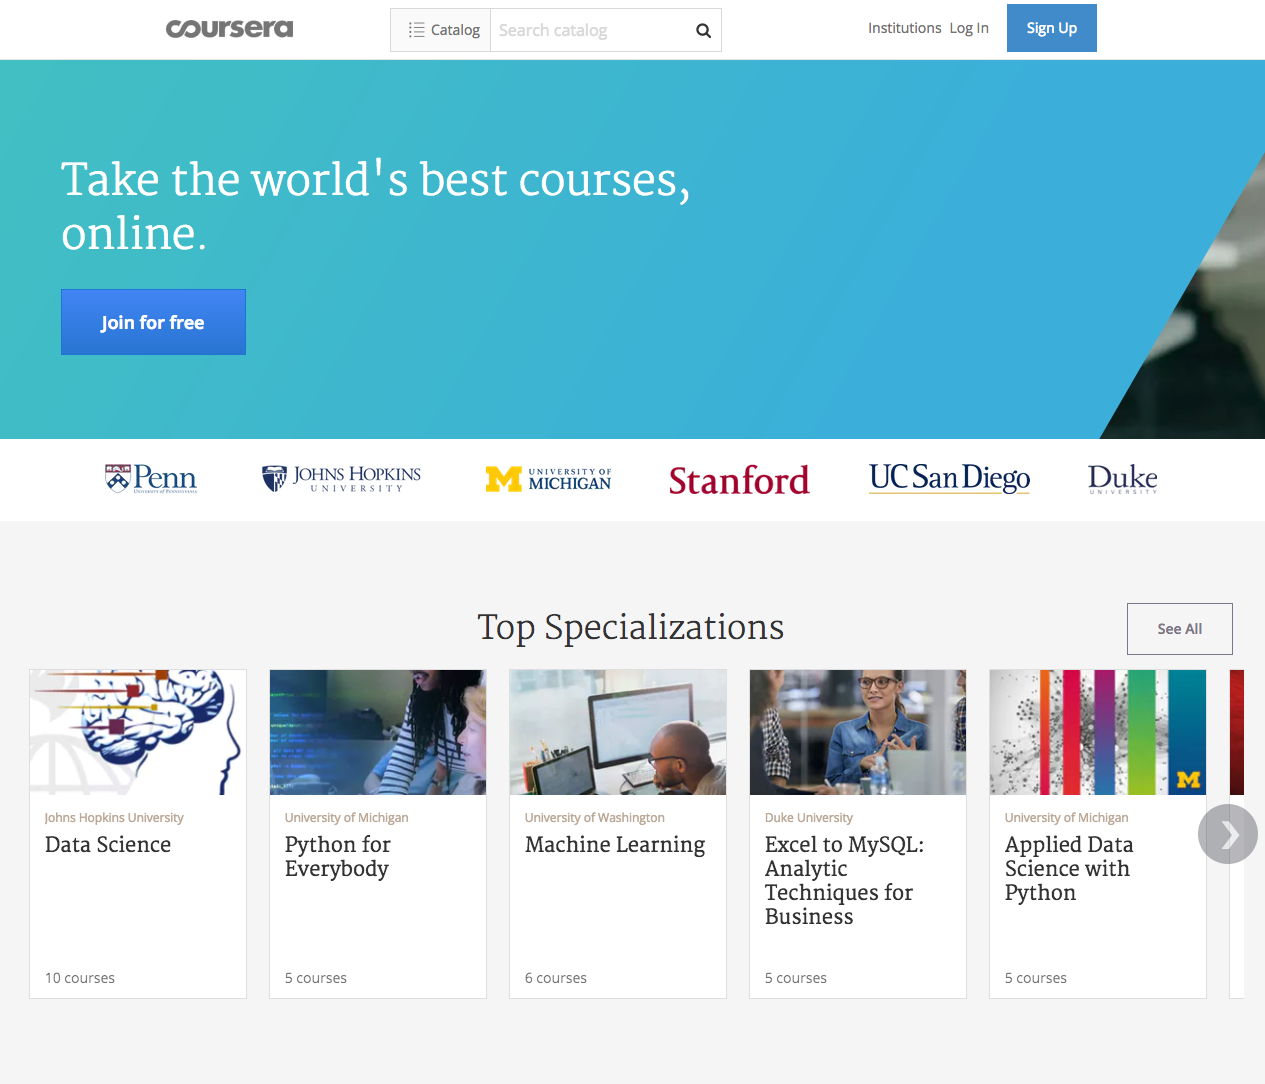
\includegraphics[width=180pt]{./img/coursera.png}
		\caption{Courseraのイメージ}
		\label{fig:cousera}
	\endminipage\hfill
	\minipage{0.53\textwidth}
		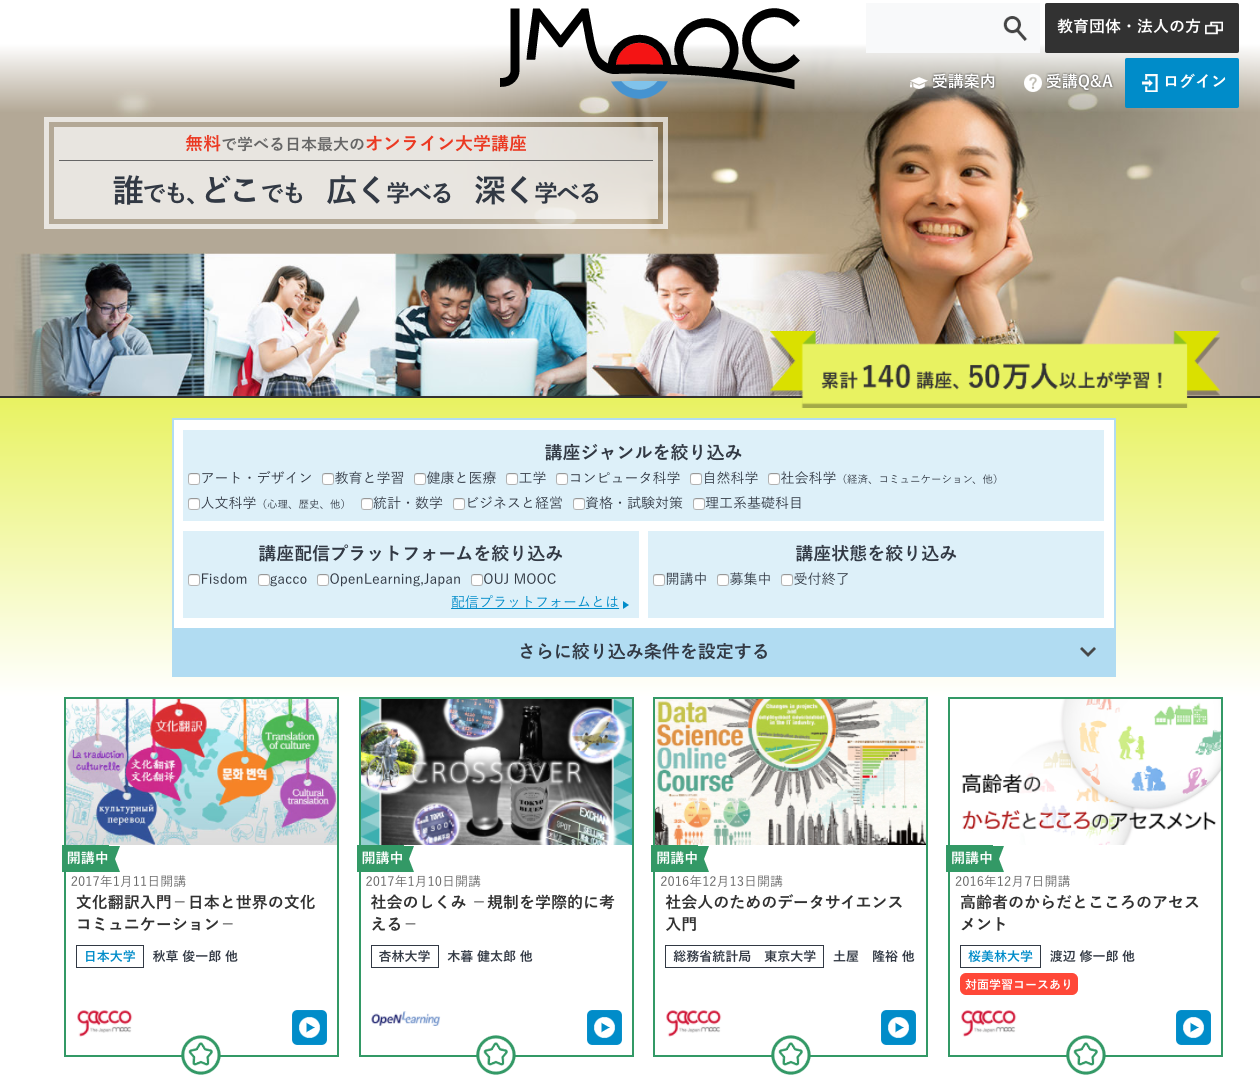
\includegraphics[width=180pt]{./img/jmooc.png}
		\caption{JMOOCのイメージ}
		\label{fig:jmooc}
	\endminipage\hfill
}
\end{center}
\end{figure}

MOOCsの有名な事例として,世界的に有名なCourseraや,日本発のMOOCsであるJMOOCが挙げられる.
CourseraとJMOOCのイメージを図\ref{fig:cousera},\ref{fig:jmooc}に示す.
Courseraは,2017年1月の時点で,
29の国にまたがる148の教育機関とパートナーシップを結び,
コンピュータサイエンス,数学や論理,社会科学などに関する1600以上の講座を,2200万人以上に提供している\footnote{講座数と利用者数はトップページの記載より引用.}.
JMOOCは,2013年11月に日本版のMOOCsとして設立され,
10代から80代までと幅広い年代に,アートや医療,自然科学や資格試験対策などの講座を提供しており,
2017年1月の時点で,140の講座を50万人以上が受講している\footnote{講座数と利用者数はトップページの記載より引用.}.



\subsection{Intelligent Tutoring System}

多様な講座を多くの人に提供するMOOCs以外にも,
より個人の学習過程をサポートすることを目的として設計された,
Intelligent Tutoring System(ITS)と呼ばれるオンライン自動学習支援システムの利用も拡大している.

\begin{figure}[htb]
\begin{center}

\includegraphics[width=200pt]{./img/knewton.png}
\end{center}
\caption{Knewtonのイメージ}
\label{fig:knewton}
\end{figure}

ITSの有名な事例として,世界最大級のITSであるKnewton\footnote{\url{https://www.knewton.com/}}のイメージを図\ref{fig:knewton}に示す.
Knewtonでは,生徒の学力や理解度と,学ぶべき対象をマッピングすることで、
生徒に最適な学習過程を設計し,
かつ生徒の学習の進捗に応じてその過程を動的に変化させる仕組みを有している\cite{upbin2012knewton}.


また,近年では,これまで難しいと言われていたITSのMOOCsへの埋め込みを達成したとする研究\cite{aleven2015beginning}も報告されており,
今後よりITSの利用は拡大していくといえる.



\subsection{学習行動ログの蓄積と大規模分析の活発化}

こうしたMOOCsやITSを始めとするオンライン教育サービスは,
人々に新たな学習の機会を提供するという側面だけでなく,
これまで難しかった大規模な学習効果分析の可能性を高めるという側面もある.

生徒はオンライン上で提供された講義動画や演習問題を通して学習するが,
オンライン上で実施されているため学習行動ログをデータとして蓄積することができ,さらに,そのデータを分析に活用することができる.
多様な生徒が利用するため,多様な生徒の大規模な学習行動ログから多様な講座の学習効果の分析が可能となりつつある.

特に,演習問題の回答ログはその演習問題により評価される知識を生徒が獲得しているか否かを表現しているため,知識獲得の分析に利用できる.
例えば,MOOCsの演習問題の回答ログを利用して知識獲得の予測を行う研究\cite{machardy2015toward}では,
世界的に有名なMOOCsであるKhan Academyから収集したデータを利用していたが,
その問題回答ログ数は100万件以上であり,
これまでにないほど大規模なデータを対象に分析が実施されたといえる.


\subsection{個人が利用するプラットフォームとしての性質}

さらに,こうしたオンライン教育サービスが学習効果分析を行う価値を大きく高めている要因として,
オンライン上のコンテンツを,多様な生徒が,個人で利用するというプラットフォームとしての性質がある.


現在の学校教育の形態では,生徒の学習効果に関する分析を行い,なんらかの知見を得たとしても,
それを多様な生徒に適用して効果を検証したり,各個人に提供できるような環境が整備されておらず,
学習効果分析が社会に与える影響が限定的であった.

また,従来のeラーニングによる学習支援システムも,
大学のような各教育機関が個別に設定し,学内の生徒が利用者の中心であったため,
システムの利用者が限定されており,データの多様性や研究成果の活用可能性も狭い範囲に留まっていた.


一方,MOOCsやITSのようなオンライン教育サービスは,
大学のような教育機関の垣根にとらわれず,多様な背景,適性,能力を持つ生徒が利用していることに加え,
学習コンテンツを個人が利用する形態のため,
多様なデータを元に得られた一般性のある知見を,多様な生徒に対して,生徒個人の粒度で提供することが可能である.
そのため,知識獲得予測を始めとする学習効果分析に基づいた,
学習の効率化や継続を促進する教材推薦システムの開発が持つ社会的影響が大きなものとなっている.


\vvspace

以上,オンライン学習サービスを取り巻く環境と,知識獲得予測研究との関連性について述べた.


次に,深層学習について述べる.


%次に,多様な研究分野に続き,教育分野の分析においてもブレークスルーを生んだ深層学習について述べるが,
%その基礎知識として機械学習やニューラルネットワークについて概説した後,
%層学習について述べる.

% 機械学習 教師あり学習と教師なし学習
% ニューラルネットワーク 活性化関数  勾配法

\section{深層学習}

本研究において用いる技術の核となっている,深層学習について述べる.
まず,深層学習を理解する必要となる周辺知識について説明した後,
深層学習の概要について述べ,
さらに本研究で用いる深層学習モデルであるRNNについて詳述する.

\subsection{深層学習にまつわる周辺知識}
深層学習について述べる前に,
深層学習を理解する上で必要となる前提知識を,以下の2つの項目に分けて述べる.

\begin{enumerate}
	\item 機械学習
	\item ニューラルネットワーク
\end{enumerate}

\subsubsection{機械学習}
(機械学習の概念,特徴量の設計,教師あり学習と教師なし学習などについて執筆予定)


\subsubsection{ニューラルネットワーク}
(ニューラルネットワークの概念,構造,活性化関数,最適化,誤差逆伝搬勾配法などについて執筆予定)


\subsection{深層学習の概要}
% - 深層学習の5W1Hについて説明
深層学習は多層のニューラルネットワークによる機械学習のことで,
従来の機械学習では,人間が問題の特徴を捉えて素性を設計する必要があったが,
深層学習では,目的に応じた素性を,最適化の過程でデータから自動で学習することが可能である.

深層学習の活用により,
画像認識\cite{schroff2015facenet,szegedy2014going},
音声認識\cite{hinton2012deep, bahdanau2015end},
会話認識\cite{sak2015fast},
機械翻訳\cite{sutskever2014sequence, dong2015multi},
質問応答文生成\cite{yin2015neural},
画像説明文生成\cite{xu2015show,vinyals2014show}等,
多様な研究領域で飛躍的な進展が報告がされている.

特に,直近の一年間だけでも
画像から動画を生成する研究\cite{vondrick2016generating}や,
会話を人間と同程度に認識できるとする音声認識の研究\cite{xiong2016achieving},
一部の欧米言語間の文レベルで,ほぼ人間と同等に正確な翻訳を実現したとする機械翻訳の研究\cite{wu2016google}などを始めとする数々の報告がされており,
深層学習によって,日々驚異的な成果が生み出されている.

また,2016年3月に人間のプロを倒したことで一躍有名になった,Google Deep Mindが開発したコンピュータ囲碁プログラムの「AlphaGo」\cite{silver2016mastering}は,
過去の人間が打った大量の棋譜に深層学習を適用した後,コンピュータ同士の対局による強化学習を通して,
今後10年は不可能と言われていた,人間のプロを打ち負かすほどの棋力を獲得した.
AlphaGoは,過去の対局の情報である棋譜の分析によって人間を真似ただけでなく,
それまで人間が考えつかなかったような手を学習しており,囲碁界に衝撃を与えている.
このように,深層学習は,人間が認識できないようなデータの複雑な特徴を捉えることで,
これまで人間が作り上げてきた概念を,大きく塗り替える可能性を秘めている.


%大規模データが必要であることに言及
一般に,深層学習モデルを学習させる際には,大規模な訓練データが必要となる.
深層学習モデルが,人の手で素性を設計していない生の訓練データから,特徴的な表現を学習し,最適化するには,
膨大な数の内部パラメータを設定して学習することが必要で,ときには数十万から数百万以上の内部パラメータが設定されることもあり,
こうした膨大な数のパラメータを学習するには,大規模な訓練データが必要となる.
データ数が不足すると,データの潜在的な特徴を十分に学習できないことに加え,
汎用性の低い特徴まで過剰に学習してしまう「過学習」に陥りやすくなる\cite{tetko1995neural}.

実際に大規模データを利用した研究の例を挙げると,
人間より高い精度で人の顔を見分けらると報告する顔認識の研究\cite{schroff2015facenet}では,
数百万人の2億枚以上の顔画像を訓練データに利用している.
英語からフランス語に翻訳する機械翻訳の研究\cite{xu2015show}では,
1200万もの文章を訓練データとして利用している.


\subsection{Recurreut Neural Networks}
% - 特に,知識獲得の予測で用いられるRNNについて5W1H
深層学習のネットワークには,目的に応じたいくつかの種類があるが,
%特に,画像処理に利用されるConvolutional Neural Networks\cite{lecun1998gradient}というネットワークと,
%系列データの処理に利用されるRecurreut Neural Networks\cite{williams1989learning}(以下,RNN)というネットワークがよく利用される.
ここでは,知識獲得の予測に深層学習を用いた手法\cite{piech2015deep}に用いられていたニューラルネットワークである,Recurreut Neural Networks\cite{williams1989learning}(以下,RNN)について説明する.


RNNは深層ニューラルネットワークの一種で,主に系列データの解析に利用される.
系列データとは,同質のデータを直列に並べて表現することにより,特定の意味を持ったデータのことで,
例えば,時系列に沿って変化する株価のようなデータや,一定の長さで順序を持って並ぶ単語からなる文章などのデータが系列データにあたる.

近年,RNNはデータの大規模化や計算機性能の向上などにより,幅広い領域の系列データに対して適用されるようになった.
具体的には,
機械翻訳\cite{sutskever2014sequence, dong2015multi},
手書き文字認識\cite{graves2009offline,louradour2014curriculum},
音声認識\cite{hinton2012deep,bahdanau2015end},
ユーザログ解析\cite{hidasi2015session},
画像説明文生成\cite{xu2015show,vinyals2014show},
医療診断\cite{choi2015doctor,lipton2015learning}等の領域で高い性能を発揮することが報告されている.

% - RNNの構造の概略
\begin{figure}[htb]
\begin{center}
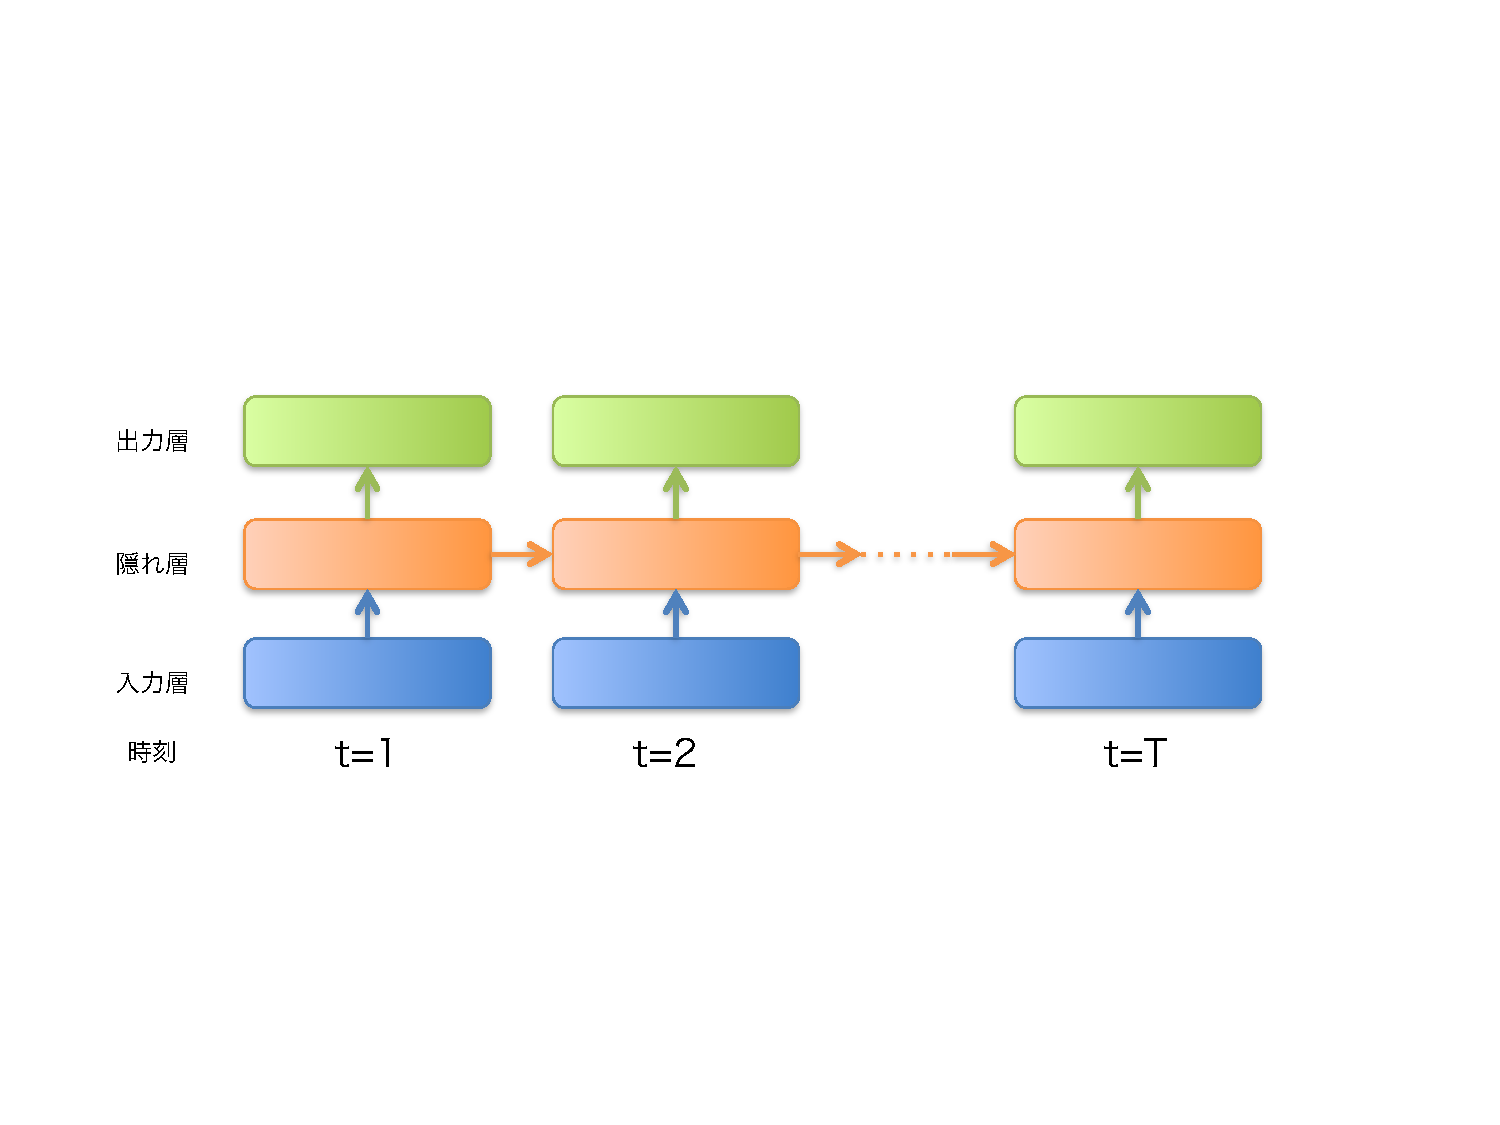
\includegraphics[width=350pt]{./img/RNN.pdf}
\end{center}
\caption{RNNの構造のイメージ}
\label{fig:RNN}
\end{figure}
伝統的なRNNの構造は図\ref{fig:RNN}のように,
入力層,隠れ層,出力層の3層から構成されている.
系列方向を時刻とすれば,
時刻$t$の隠れ層${\bf h}_t$の計算に時刻$t-1$の隠れ層の情報を入力する${\bf h}_t = f({\bf x}_t, {\bf h}_{t-1})$の式ように,一つ前の情報を繰り返し(recurrent)入力するという構造である.
関数$f$は,入力である${\bf x}_t$や${\bf h}_{t-1}$をアフィン変換\footnote{平行移動と線形変換を組み合わせた変換のこと.}して足しあわせた後,活性化関数にかけるというものがよく利用される.
活性化関数はシグモイド関数やtanh(Hyperbolic Tangent関数),Relu\cite{nair2010rectified},ELUs\cite{clevert2015fast}など多く提案されており,通常,非線形関数である.



% - RNNの課題について説明
このように,データの系列に沿った情報を反映して学習できるRNNだが,
課題の一つとして,長期的な表現になるほど学習が難しくなるということが挙げられる\cite{bengio1994learning}.
RNNの学習には,勾配法に基づいた確率的勾配降下法\cite{robbins1951stochastic,kushner2003stochastic}やAdam\cite{kingma2014adam},AdaDelta\cite{zeiler2012adadelta}など,さまざまな手法が利用可能である.
しかし,いずれの勾配法を用いるにせよ,
勾配が爆発して学習モデルが壊れてしまうという勾配爆発\cite{bengio1994learning,pascanu2013difficulty}という問題や,
勾配が消滅して対象データの長期的な特徴量を捉えることができないという勾配消滅\cite{pascanu2013difficulty, hochreiter1998vanishing}という問題がしばしば発生する.
これは,
${\bf h}_t = f({\bf x}_t, {\bf h}_{t-1})$の式に表れるように同じ変換を繰り返し行うためであり,
このため,特に長い系列データをRNNで学習する場合,効果的に長期的な表現を学習させることが難しい.


% - 課題解決の手法について説明
こうした問題を解決もしくは緩和するため,学習時の勾配に制約を加える方法やゲート付き活性化関数の利用が提案されている.
まず,勾配爆発の緩和に対しては,学習時の勾配に制約を加える方法が有効である.
具体的には,
\cite{mikolov2012statistical}では
学習させるパラメタの勾配の絶対値の最大値を予め決めておき,
最大値以上の場合には,勾配の最大値になるように勾配の値を置き換えることで勾配爆発の影響を緩和する方法が報告された.
また,
\cite{pascanu2013difficulty}では
学習させるパラメタの勾配のノルムの最大値を予め決めておき,
最大値以上の場合には, ノルムが最大値以下になるように疑似コード\ref{normregular}に従いノルムを抑制することで勾配爆発の影響を緩和する方法が報告された.
\begin{algorithm}                      
\caption{勾配爆発を防ぐための勾配ノルム抑制の疑似コード}
\label{normregular}                          
\begin{algorithmic}                  
	\STATE $\hat{{\bf g}} \leftarrow \frac{\delta \varepsilon}{\delta {\bf \theta}}$
	\IF{$\Vert \hat{{\bf g}} \Vert \geq threshold $}
	\STATE $\hat{{\bf g}} \leftarrow \frac{threshold}{\Vert \hat{{\bf g}} \Vert} \hat{{\bf g}}$
	\ENDIF
\end{algorithmic}
\end{algorithm}


次に,勾配消滅の緩和に対しては,ゲート付き活性化関数の利用が有効である.
先に,言及したが,RNNには異なる活性化関数を利用するという形でいくつかの種類がある.
うまく設計された活性化関数を利用することで,勾配消滅を緩和してデータの長期的な特徴をよく捉えられたり,計算コストを削減することができたりする.
以降では,よく研究報告で取り上げられるSimple RNN(以下,SRNN)\cite{williams1989learning},Long Short  Term Momory RNN(以下,LSTM-RNN)\cite{hochreiter1997long},Gated Recurrent Neural Networks(以下,GRNN)\cite{cho2014learning}の3つについて詳細に説明する.



\subsubsection{SRNN}
SRNNはゲート付き活性化関数を用いない簡単な構造のRNNである.
\cite{le2015simple, krueger2015regularizing}で報告される工夫を取り入れることで,データの長期的な特徴を効果的に捉えることができるようになるが,
多くの場合で,LSTM-RNNやGRNNのようにゲート付き活性化関数を用いるRNNの方がモデルの性能という点で優れている.

SRNNによるモデルの定式はいくつか種類が存在するが,シンプルなものは例えば下記の式で定義される.
\begin{eqnarray}
\label{eq:srnn1}
{\bf h}_t &=& \tanh({\bf W}_{xh} {\bf x}_t + {\bf W}_{hh}  {\bf h}_{t-1} + {\bf b}_h)\\
\label{eq:srnn2}
{\bf y}_t &=& \sigma( {\bf W}_{hy} {\bf h}_t + {\bf b}_y)
\end{eqnarray}
ここでは,
$t$は時刻を指し,
${\bf x}_t$は時刻$t$の入力ベクトルを指し,
${\bf h}_t$は時刻$t$の隠れ層を指し,
${\bf y}_t$は時刻$t+1$の各問題の正誤確率の予測値を指し,
${\bf W}_{xh}$,${\bf W}_{hh}$はそれぞれ重み行列を指し,
${\bf b}_h$,${\bf b}_y$はそれぞれバイアス項を指し,
$\tanh$は$( e^x - e^{-x} )/( e^x + e^{-x} )$で定義されるHyperbolic Tangent関数を指し,
$\sigma$は$1 / (1 + e^{-x})$で定義されるシグモイド関数を指す.
訓練時には,重み行列${\bf W}_{xh}$,${\bf W}_{hh}$とバイアス項${\bf b}_h$,${\bf b}_y$を学習する.


\subsubsection{LSTM-RNN}
LSTM-RNNはLong Short Term Memoryという活性化関数を用いるRNNで,
その名前の通り,SRNNでは捉えることが難しかったデータの長期的表現と短期的表現の両方の獲得を目的に開発されたものである\cite{hochreiter1997long}.
LSTM-RNNはSRNNと比較すると,モデルの性能という点で優れているが,内部のパラメタの数が非常に大きく学習コストは大きい.
最先端の成果を報告する研究でしばしば利用されているが,
LSTM-RNN自体が開発されたのは1997年でありLSTN-RNNが新しいというわけではない.

LSTM-RNNによるモデルの定式にはいくつか種類が存在するが,特に,後述するDeep Knowledge Tracing\cite{piech2015deep}で用いられるLSTM-RNNは下記の式で定義される.
\begin{eqnarray}
\label{eq:lstmrnn1}
{\bf i}_t &=& \sigma({\bf W}_{xi}{\bf x}_t + {\bf W}_{hi}{\bf h}_{t-1} + {\bf b}_i) \\
\label{eq:lstmrnn2}
{\bf g}_t &=& \sigma({\bf W}_{xg}{\bf x}_t + {\bf W}_{hg}{\bf h}_{t-1} + {\bf b}_g) \\
\label{eq:lstmrnn3}
{\bf f}_t &=& \sigma({\bf W}_{xf}{\bf x}_t + {\bf W}_{hf}{\bf h}_{t-1} + {\bf b}_f) \\
\label{eq:lstmrnn4}
{\bf o}_t &=& \sigma({\bf W}_{xo}{\bf x}_t + {\bf W}_{ho}{\bf h}_{t-1} + {\bf b}_o) \\
\label{eq:lstmrnn5}
{\bf m}_t &=& {\bf f}_t \odot {\bf m}_{t-1} + {\bf i}_t \odot {\bf g}_t \\
\label{eq:lstmrnn6}
{\bf h}_t &=& {\bf o}_t \odot {\bf m}_t  \\
\label{eq:lstmrnn7}
{\bf y}_t &=& \sigma({\bf W}_{my} {\bf m}_t + {\bf b}_y) 
\end{eqnarray}
ここでは,
${\bf i}_t$はInput Gateを指し,
${\bf f}_t$はForget Gateを指し,
${\bf g}_t$はメモリセルへの入力を指し,
${\bf o}_t$はOutput Gateを指し,
${\bf m}_t$はメモリセルを指し,
${\bf W}_{xi}$,${\bf W}_{hi}$,
${\bf W}_{xg}$,${\bf W}_{hg}$,
${\bf W}_{xf}$,${\bf W}_{hf}$,
${\bf W}_{xo}$,${\bf W}_{ho}$,
${\bf W}_{my}$
はそれぞれ重み行列を指し,
${\bf b}_i$,${\bf b}_g$,${\bf b}_f$,${\bf b}_o$,${\bf b}_y$はそれぞれバイアス項を指し,
$\odot$は要素積を指す.

式\ref{eq:lstmrnn5}にあるように,メモリセルへの入力は1つ前のメモリセルの状態${\bf m}_{t-1}$と入力${\bf g}_t$であり,
それぞれの入力に対して,過去のメモリセルからの情報を捨てるForget Gateと現在からの情報を調整するInput Gateを作用させ,${\bf m}_t$をえる.
新しい隠れ層${\bf h}_t$は式\ref{eq:lstmrnn6}のようにメモリセルからの出力をOutput Gateで調整したものを入力として受け取る.
これらのゲートにより,
長期的な特徴の短期的な特徴が捉えられるとされている.

\subsubsection{GRNN}
GRNNはGated Recurrent Unit\cite{cho2014learning}というゲート付き活性化関数を用いるRNNのことで,
GRUはLSTMのように,長期的な表現と短期的な表現を捉えるために提案された活性化関数である.
Choら\cite{cho2014learning}が2014年に発表して以来,GRNN自体やGRNNの活用に関する研究が多く報告されている\cite{chung2014empirical, zaremba2015empirical, chung2015gated, karpathy2015visualizing, biswassentiment, pezeshki2015sequence}.
LSTMよりもゲートの数が少なく学習コストが小さい傾向にあるが,
LSTM-RNN,GRNNの性能を比較した研究\cite{chung2014empirical, zaremba2015empirical}においてLSTM-RNNとGRNNが同程度の性能であることが報告されている.

GRNNは下記の式により定義される.
\begin{eqnarray}
\label{eq:grurnn1}
{\bf r}_t &=& \sigma({\bf W}_{xr}{\bf x}_t + {\bf W}_{hr}{\bf h}_{t-1} + {\bf b}_r)\\
\label{eq:grurnn2}
{\bf z}_t &=& \sigma({\bf W}_{xz}{\bf x}_t + {\bf W}_{hz}{\bf h}_{t-1} + {\bf b}_z)\\
\label{eq:grurnn3}
\tilde{{\bf h}}_t &=& \tanh({\bf W}_{xh}{\bf x}_t + {\bf W}_{hh}({\bf r}_t \odot {\bf h}_{t-1} + {\bf b}_h))\\
\label{eq:grurnn4}
{\bf h}_t &=& {\bf z}_t \odot {\bf h}_{t-1} + (1 - {\bf z}_t) \odot \tilde{{\bf h}}_t\\
\label{eq:grurnn5}
{\bf y}_t &=& \sigma( {\bf W}_{hy} {\bf h}_t + {\bf b}_y)
\end{eqnarray}
ここでは,
${\bf W}_{xr}, {\bf W}_{hr}, {\bf W}_{xz}, {\bf W}_{hz}, {\bf W}_{xh}, {\bf W}_{hh}$は重み行列で, 
${\bf b}_r, {\bf b}_z, {\bf b}_h$はバイアス項である.
${\bf r}_t$がReset Gate(LSTMにおけるForget Gateに相当する機構)で,  
${\bf z}_t$がUpdate Gate(LSTMにおけるメモリセルに相当する機構)である.
${\bf r}_t$が0に近いほど前の隠れ層からの入力よりも現在の入力をより強く考慮するようになり,
${\bf z}_t$が0に近いとほど前の隠れ層をより大きく更新するようになる.


\vvspace


以上,周辺知識を整理した上で深層学習について述べ,本研究と関連の深いRNNについて詳述することで,技術的な前提知識を確認した.

次に,知識獲得の予測について述べる.



\section{知識獲得の予測}
% - 知識獲得の予測について5W1H(what, when, who, why, where, how)
知識獲得の予測は,生徒が対象の知識を獲得しているか否かを予測する問題である.
通常,知識を獲得しているか否かは問題回答の正誤を基に評価されるため,
知識獲得の予測のタスクは過去の生徒の問題回答履歴から次に解く問題の正誤を予測するというものである.

最初の定式化の事例は,1994年にCorbettらによって報告されたKnowledge Tracing\cite{corbett1994knowledge}である.
スキルの習熟学習において,
領域知識をよく分析し階層的に知識間関係を構築し,
階層構造においてより水準の高い知識に着手する前に予め獲得するべき知識が確実に獲得されるように学習体験を設計することで,
ほとんどの生徒がスキルを十分に習熟できるとする仮説\cite{keller1968good, bloom1968learning}や,
コンピュータサイエンスの発展を受けて,
予め獲得すべき知識が確実に獲得されるように生徒の知識の獲得有無を予測するというのが主な目的であった.
Knowledge Tracingにおける生徒とモデルは,生徒が勉強し知識を獲得したら,モデルが生徒が獲得した知識を予測することで生徒の獲得している知識の変化を追跡する({\it Knowledge Tracing}),という関係になっている.


% - 伝統的には2つのアプローチがあることを説明
伝統的に,知識獲得の予測には知識獲得の時系列性を重視するものと,知識間の関係性を重視するものがある.
\cite{corbett1994knowledge}で報告されたBayesian Knowledge Tracingという手法は知識獲得の時系列性を重視するもので,
問題に予めスキルを割り当て個々のスキルに習熟過程に関する4つの確率変数を定義しモデル化するというもので,
スキル間の関係性は考慮しないが,個々のスキルの習熟,つまり時系列性を考慮する手法である.
\cite{pavlik2009performance}で報告されたPerformance Factor Analysisという手法は知識間の関係性を重視するもので,
個々の知識(あるいは,スキル)に関する過去の回答の正誤を重み付けして,次の問題の正誤を予測しようというもので,
Performance Factor Analysisは知識獲得の時系列性より知識間の関係性を重視する手法である.
いずれの手法も本論文と関連が深い.


以降では,まず,Knowledge Tracingの定式化について述べ,
Bayesian Knowledge TracingとPerformance Factor Analysisの2つの手法を説明し,
最後に,深層学習を活用したDeep Knowledge Tracingについて説明する.


\subsection{Knowledge Tracingの定式化}
Knowledge Tracingは過去の生徒の問題回答履歴から生徒が次に解く問題の正誤を予測するというものである.
生徒の時刻$t$において観測された問題回答結果を$q_{t}$とすれば,
$q_1, q_2, \dots, q_t$から時刻$t+1$において観測される問題回答結果$q_{t+1}$を予測するタスクと表現できる.
特に,過去の観測された問題の正誤から将来の正誤確率を算出する場合は,
$q_1, q_2, \dots, q_t$が観測された場合の時刻$t+1$に着手する問題において当該生徒の回答正解となる事後確率
$p(q_{t+1} = correct|q_1, q_2, \dots, q_t)$を求めるタスクであるといえる.
予測性能の評価は\cite{yudelson2013individualized, falakmasir2015spectral}ではAccuracy\footnote{正解率.予測結果全体と、答えがどれぐらい一致しているかを判断する指標.0〜1で表され,完全な予測時に1となる.}で,
\cite{piech2015deep}ではAUC\footnote{正例を正しく分類した割合を縦軸に,負例を正しく分類した割合を横軸に取るROC曲線における,曲線より下の面積.0〜1で表され,完全な予測時に1となり,ランダムな予測で0.5付近を示す.}で行っており,
目的に応じてさまざまである.
本研究では,AUCによって予測性能を評価する.


なお,モデルの入力次元である「問題」の粒度はさまざまである.
問題はその問題を回答するのに必要な知識を生徒が獲得しているか否かを評価するという点で,
問題は知識集合を表現しており,また,その粒度もさまざまである.
個々の問題をそのままモデルの入力次元とするものや,問題に予めタグを割り当て問題により評価される知識の粒度をある程度整え,そのタグをモデルの入力次元とすることもある.
例えば,
\cite{piech2015deep}ではモデルの入力次元は演習タグもしくはスキルタグと呼ばれるものであり,
演習問題に割り当てられ,それぞれの演習問題で扱われる学習要素を説明するものである.
通常,こうしたタグは専門家によって設計され,利用される.
本論文では個々の問題をそのままモデルの入力次元として用いる.


\subsection{Bayesian Knowledge Tracing}
Bayesian Knowledge Tracing\cite{corbett1994knowledge}(以下,BKT)はベイズの定理の事前確率と事後確率の関係に基づいて正解確率$p(q_{t+1} = correct|q_1, q_2, \dots, q_t)$をモデリングする手法である.
BKTには下記の4つの確率変数がある.
\begin{itemize}
\item 初めから当該スキル理解している確率$p(L_0)$(もしくは $p\mhyphen init$)
\item 生徒が当該スキルを理解していない状態から理解している状態へ遷移する確率$p(T)$(もしくは $p\mhyphen transit$)
\item 生徒が当該スキルを理解しているが誤答する確率$p(S)$(もしくは $p\mhyphen slip$)
\item 生徒が当該スキルを理解していないが推測で正解する確率$p(G)$(もしくは $p\mhyphen guess$)
\end{itemize}
これらの4つの確率変数がすべてのスキルに定義されている.つまり,スキル数を$N$とすれば,確率変数の合計数は$4N$である.
生徒$u$がスキル$k$の問題を時刻$t$に解いた場合に正解する確率は下記の式に基づいて更新される.

\hspace*{-55pt}\minipage{1.1\textwidth}
\begin{eqnarray}
\label{eq:bkt_update1}
p(L_1)^{k}_{u} &=& p(L_0)^k \\[\eqnsp]
\label{eq:bkt_update2}
p(L_{t}|obs=correct)^{k}_{u} &=& \frac{ p(L_{t-1})^{k}_{u} \cdot (1 - p(S)^k) }{ p(L_{t-1})^{k}_{u} \cdot (1 - p(S)^k) + (1 - p(L_{t-1})^{k}_{u}) \cdot p(G)^k } \\[\eqnsp]
\label{eq:bkt_update3}
p(L_{t}|obs=wrong)^{k}_{u} &=& \frac{ p(L_{t-1})^{k}_{u} \cdot p(S)^k }{ p(L_{t-1})^{k}_{u} \cdot p(S)^k + (1 - p(L_{t-1})^{k}_{u}) \cdot (1 - p(G)^k) } \\[\eqnsp]
\label{eq:bkt_update4}
p(L_{t})^{k}_{u} &=& p(L_{t}|obs)^{k}_{u} + (1 - p(L_{t}|obs)^{k}_{u}) \cdot p(T)^k  \\[\eqnsp]
\label{eq:bkt_update5}
p(C_{t})^{k}_{u} &=& p(L_{t-1})^{k}_{u} \cdot (1 - p(S)^k) + (1 - p(L_{t-1})^k_{u}) \cdot p(G)^k
\end{eqnarray}
\endminipage\hfill
%}
\vvspace
\vvspace


右上の$k$はスキル番号を示し,右下の$u$はユーザ番号を示すことに注意されたい.
まず,生徒$u$が初めから当該スキル$k$を身につけている確率は式\ref{eq:bkt_update1}の通り定義する.
正解が観測され,正しく当該スキルを身につけている確率は,式\ref{eq:bkt_update2}で与えられ,
不正解が観測されたが,正しく当該スキルを身につけている確率は,式\ref{eq:bkt_update3}で与えられ,
それらを合わせて,次の時刻に当該スキルを身につけている確率は,式\ref{eq:bkt_update4}で与えられる.
このように定めることで,理解しているがうっかり間違ってしまう場合や, 理解していないがあてずっぽうで正解してしまう場合を考慮できる.
なお当該モデルでは,身につけたスキルの忘却は無視している.
最後に,生徒$u$がスキル$k$の問題を時刻$t$に解いた場合に正解する確率$p(C_{t})^{k}_{u}$は式\ref{eq:bkt_update5}のように算出され,
この値を次の問題の正誤予測に利用する.
 
上記に説明したモデルの学習にはいくつかの方法が適用され報告されている.
1つは\cite{corbett1994knowledge}にあるようにHMMを用いて生成モデルとして学習させる方法であり,
1つは\cite{yudelson2013individualized}にあるように勾配法を用いて識別モデルとして学習させる方法である.
それぞれ長所と短所があるが,
特に,大規模データへの適用という観点ではHMMに基づいた生成モデルの手法では計算量が大きく学習に非常に多くの時間がかかってしまうということもあり,
\cite{yudelson2013individualized}では勾配法に基づいた識別モデルとして学習させている.
具体的には,\cite{yudelson2013individualized}では,目的関数に負の対数尤度(Negative Log Likelihood)を利用し,勾配降下法(Gradient Descent)で学習させている.
%本論文で扱うデータは大規模であるため,学習方法は識別モデルとして扱う場合について説明した.
%生成モデルとして扱う場合の学習方法については\cite{corbett1994knowledge}を参照されたい.



\subsection{Performance Factor Analysis}
Performance Factor Analysis\cite{pavlik2009performance}(以下,PFA)も
過去の生徒の問題回答履歴から生徒が次に解く問題の正誤を予測するための手法である.
しかし,
知識獲得の時系列性を考慮するBKTと異なり,
知識獲得の順番を考慮せず知識間の関係性を考慮して予測する手法である.
PFAは下記のように定義される.
\begin{eqnarray}
	p(i, j \in KCs, s, f) & = & \sigma( \beta _j + \sum_{k \in KCs}(\gamma_k s_{i, k} + \rho _k f_{i, k}) )
\end{eqnarray}
ここでは,
$s$は事前に正答した問題回答,
$f$は事前に誤答した問題回答,
$p$はユーザ$i$が知識$j$に正答する確率,
$\beta_j$は知識$j$の簡単さ,
$\gamma_k$と$\rho_k$はそれぞれ知識$k$の正答と誤答の重み,
$s_{i, k}$と$f_{i, k}$はそれぞれユーザ$i$が知識$k$に事前に正答した問題回答,事前に誤答した問題回答
である.
$\sigma$はシグモイド関数,
過去の各知識の正誤を重み付けしシグモイド関数にかけ,別の問題の正誤を予測するというものである.

%特に,深層学習を用いる前のKnowledge Tracingでは
%問題回答の順番を考慮していたが知識間の関係性は考慮する研究は著者の知る限り\cite{kaser2014beyond}の以外ない.
PFAは
知識間の関係性を考慮できない場合に複数の知識がないと獲得できない知識のモデルが難しいという
Bayesian Knowledge Tracingやその拡張手法の問題を解決するために
提案された.
PFAは知識間の関係性を重み付けして考慮しているが,
問題回答の順番は考慮しない.


\subsection{Deep Knowledge Tracing}
Deep Knowledge Tracing\cite{piech2015deep}(以下,DKT)はRNNを利用しKnowledge Tracingを行う手法である.
2015年6月に発表された.
数学の問題回答ログのデータセットで実験され,
高い性能で将来の知識獲得を予測できること,
予測モデルを分析することで知識間関係をネットワークとして抽出できることが報告された.
生徒が獲得している知識から,ある知識の獲得されやすさをそのまま予測しており,
得られた知識間関係から抽出されたネットワークは知識獲得における知識構造を表現しているといえる.
DKTの構造と最適化,および知識間関係の抽出手法について順に説明していく.



\subsubsection{構造}
まず,DKTの構造について述べる.
DKTの構造は伝統的なRNNの構造に基づいている.
伝統的なRNNは入力のベクトル系列${\bf x}_1, \dots, {\bf x}_T$を出力のベクトル系列${\bf y}_1, \dots, {\bf y}_T$に写像する.
この写像は,隠れ状態${\bf h}_1, \dots, {\bf h}_T$を計算することで達成されるが,一連の写像の過程で過去観測から得られる関連情報を将来予測のために連続的に符号化している,とみなせる.確率変数は下記の式で定義されるネットワークにより関連付けられる.
\begin{eqnarray}
\label{eq:rnn1}
{\bf h}_t &=& f({\bf x}_t, {\bf h}_{t-1})\\
\label{eq:rnn2}
{\bf y}_t &=& g({\bf h}_t)
\end{eqnarray}
モデルは関数$f$と$g$によって定義されており,
これらの関数$f, g$にはSRNNの式\ref{eq:srnn1},\ref{eq:srnn2}やLSTM-RNNの式\ref{eq:lstmrnn1}--\ref{eq:lstmrnn7},GRNNの式\ref{eq:grurnn1}--\ref{eq:grurnn5}を利用できる. 


RNNで生徒の学習行動の観測結果をモデリングするため観測結果を固定長の入力ベクトル${\bf x}_t$の系列に変換する必要があるが,DKTではシンプルな変換を行っている.具体的には,生徒の学習行動の観測結果をone-hotベクトルに符号化し${\bf x}_t$とする,というものである.
観測結果は演習問題と正誤の組み合わせで表現できるため,演習問題の数を$M$とすれば,${\bf x}_t$の長さは$2M$となる.


\begin{table}[ht]
\caption{Deep Knowledge Tracingにおける回答ログデータと対応する入力ベクトルの例}
\label{tab:samplelog}
\begin{center}
\centerline{
{
\begin{tabular}{crrr|cc}\hline\hline
	\multicolumn{4}{c|}{回答ログ}	&	\multicolumn{2}{c}{入力ベクトル}	\\
	ユーザID	&	ログの順番	&	問題番号	&	正誤	&	変数名			&	値											\\\hline
	A			&	1			&	1			&	0		&	${\bf x}_1$ 			& $[0 0 0 0 \vdots 1 0 0 0 ]$	\\
	A			&	2			&	1			&	1		&	${\bf x}_2$ 			& $[1 0 0 0 \vdots 0 0 0 0 ]$	\\
	A			&	3			&	2			&	1		&	${\bf x}_3$ 			& $[0 1 0 0 \vdots 0 0 0 0 ]$	\\
	A			&	4			&	3			&	0		&	${\bf x}_4$ 			& $[0 0 0 0 \vdots 0 0 1 0 ]$	\\
	A			&	5			&	3			&	1		&	${\bf x}_5$ 			& $[0 0 1 0 \vdots 0 0 0 0 ]$	\\
	A			&	6			&	4			&	1		&	${\bf x}_6$ 			& $[0 0 0 1 \vdots 0 0 0 0 ]$	\\
\hline\hline
\end{tabular}
}
}
\end{center}
\end{table}


具体例を交えて説明する.
例えば,演習問題の数が4つで,問題回答は1つずつしかできないと仮定する .$M=4$であり,${\bf x}_t$の長さは$8$である.
ある生徒が,表\ref{tab:samplelog}の回答ログように問題を回答し正誤が観測されたとする.
この時に,例えば,表\ref{tab:samplelog}に記載のような入力ベクトルの系列となる.
このようにして,回答行動の観測結果を符号化することで,どの演習問題をいつ正解もしくは不正解したのかをRNNに入力できる.

出力${\bf y}_t$は問題と同じ長さのベクトルで,
それぞれの要素が当該生徒がそれぞれの問題に正しく回答する確率の予測値となっている.
したがって,$t+1$の回答$q_{t+1}$の正誤予測は$t+1$に回答される問題$q_{t+1}$に対応する${\bf y}_t$の要素から読み取れる.


\subsubsection{最適化}
次に,DKTの最適化について述べる.
訓練時に用いられる目的関数は,
モデルにおいて生徒の回答行動の観測系列の負の対数有度(Negative Log Likelihood)である.
${\bf \delta}(q_{t+1})$を時刻$t+1$にどの問題が回答されたかのone-hotベクトルとし,
$a_{t+1}$を時刻$t+1$に当該問題で正答したか否か($1$か$0$)とし,
$l$をクロスエントロピーとすれば,
当該予測結果に対するロス関数は $l({\bf y}^T {\bf \delta}(q_{t+1}), a_{t+1})$であり,
生徒一人のロスは下記の式で与えられる.
\begin{eqnarray}
L &=& \sum_t l({\bf y}_t^T {\bf \delta}(q_{t+1}), a_{t+1})
\end{eqnarray}


学習時はミニバッチごとに確率的勾配降下法で目的関数を最小化する.
\cite{piech2015deep}では,モデル学習時には過学習を防ぐため${\bf y}_t$への入力としての${\bf h}_t$にはdropout\cite{srivastava2014dropout}を適用している(${\bf h}_{t+1}$の方向にはdropoutを適用しない).
また,系列方向の誤差逆伝搬\cite{werbos1990backpropagation}において勾配が爆発するのを防ぐため,閾値以上のノルムの勾配は\cite{pascanu2013difficulty}にしたがい,制約を設けている.


\subsubsection{知識間関係抽出法}
次に,DKTのモデルを利用した知識間関係(あるいは,問題間関係)抽出法について述べる.
DKTのモデルは,従来ではよく人間の専門家が行っていたデータの潜在的な構造や概念を発見するタスクに応用できる.
問題$i$と$j$のすべての有向ペアのうち下記の条件を満たすものに対して下記の影響度$J_{ij}$を割り当てる.\\
\begin{itemize}
	\item [条件]有効ペア$(i, j)$について,問題$i$が出現した後に残りの問題系列の中で問題$j$が出現する系列数が問題$i$が出現する問題系列数全体の$V\%$以上であること.
	\item[影響度]
$$J_{ij} = \frac{y(j|i)}{\sum_k y(j|k)}$$\\
\end{itemize}
ここでは,$y(j|i)$は,ある生徒が最初に問題$i$に正答した場合に,RNNによって割り当てられる次の時刻に問題$j$に正答する確率である.
\cite{piech2015deep}では,問題間影響行列からのネットワーク抽出には,
$V=1$を用いた.
また,ネットワークの可視化に際しては,影響度が$0.1$以上であればエッジを引くというようにしてネットワークを構築した.

さらに,\cite{piech2015deep}は,
得られたネットワークは,
単に生徒の問題$(i, j)$間の遷移率から構築したネットワークや
問題$i$の正解が観測された後に問題$j$の正解が観測される条件付き確率から構築したネットワークより
よく知識間関係を捉えていることを指摘している.


こうして得られた行列$J$は,
問題$i$で評価される知識が既に獲得されている場合に,
問題$j$で評価される知識の獲得されやすさを表現しており,
$J$は知識間関係行列であるといえ,
この知識間関係行列から構築したネットワークは
知識獲得における知識構造を表現していると考えられる.


\subsection{知識獲得予測の手法におけるDKTの最適性}

ここまで知識獲得予測の様々な手法について述べたが,
DKTを拡張する手法が,本研究の目的を達成する上で最適な手法であることを,以下の二点に基づいて説明する.
1)知識間の関係性は,知識獲得予測の文脈において,定量的に検証されて抽出されるべきこと,
2)知識獲得予測は,複数の知識間の影響関係や,知識獲得の時系列性を考慮して行われるべきこと,


まず,1について述べる.
知識間の関係性は,知識獲得予測の過程で抽出されるものと,そうでないものがある.
後者については,
専門家が作成するという手法や,
テキスト解析により概念関係ネットワークを構築するという手法\cite{chen2008mining}がある.
しかし,これらの手法は,
専門家や研究者が立てた仮説に基づいた定性的なものであり,
実際の生徒の学習過程をよく説明するものであるという定量的な根拠はない.

問題回答正誤の分析により知識の構造化を行う方法[参考文献引用]も,%詳述
2つの問題$i$と$j$の間で問題$i$が正解後と不正解後の問題$j$の正解率の差と着手順序を基に知識を構造化するが,
この手法は2つの問題$i$と$j$の関係性のみを考慮しており,他の問題との関係性は独立だと見なされている.
得られた知識間関係は2つの知識の間についてのものを線形に合算したものであり,
複雑で密接に関係している複数の知識の獲得順序や影響関係を捉えているものではない.

一方で,知識間の関係性の抽出を,知識獲得を予測する過程で行うものは,
生徒の知識状態と行動を元に,知識の獲得を予測しているため,
生徒の学習過程を反映した知識間関係を表現している可能性が高い.

したがって,
知識間関係を定量的に抽出する手法としては,
知識獲得を予測する過程で知識間関係を抽出する手法に絞る.


次に,2について述べる.
知識獲得予測には,
複数の知識の影響関係や知識獲得の時系列性を考慮するものと,そうでないものがある.
% BKT的なものとDKT的なものがある
後者については,
複数の知識を独立なものとして,それらの状態の遷移を定義するBayesian Knowledge Tracing(BKT)の手法や,
過去の回答の結果を1つにまとめて定義するPerformance Factor Analysis(PFA)の手法などがある.
しかし,BKTの手法は,複数の知識を独立なものとして捉えるため,複数の知識からなる複雑な知識状態を捉えきれず,
また,PFAの手法は,直前の回答も十分な時間が立った後の回答も,一つの過去の回答として捉えるため,
生徒の時間に沿った知識獲得の状態を,現実的に捉えきれていない.

一方,DKTは,時系列に沿ってRNNの隠れ層を更新することにより,
複数の知識間の影響関係や,知識獲得の時系列性を考慮して知識獲得を予測しているので,
より現実に沿った知識間関係を抽出できる可能性が高い.

現に\cite{piech2015deep}で,
既にDKTによって知識間関係を抽出できることが報告されており,
複雑で密接に関係している複数の知識の獲得順序や影響関係を捉えている可能性が高く,
DKTを利用することが最適であると考えられる.

% PFAについては述べる必要ないかも
また,PFAとDKTのいずれの手法も知識間関係を考慮して予測に利用しているが,DKTの方が有効性が高いと考える.
なぜなら,
\cite{piech2015deep}では言及されていなかったが,
DKTはPFAの拡張になっているためである.
DKTはRNNを利用しており,
\begin{eqnarray}
{\bf h}_t & = & f({\bf x}_t, {\bf h}_{t-1})\\
{\bf p}_t & = & \sigma({\bf h}_{t-1} \cdot {\bf W}_{hp} + {\bf b}_p)
\end{eqnarray}
で与えられる.
一方でPFAは
\begin{eqnarray}
	p(i, j \in KCs, s, f) & = & \sigma( \beta _j + \sum_{k \in KCs}(\gamma_k s_{i, k} + \rho _k f_{i, k}) )
\end{eqnarray}
で与えられる.
したがって,
\begin{eqnarray}
\label{eq:discussion-func}
	f({\bf x}_t, {\bf h}_{t-1}) &=& {\bf x}_t + {\bf h}_{t-1}\\
	{\bf h}_{0} & = & [0, 0, \cdots , 0]
\end{eqnarray}
とすると,
${\bf h_t}$がこれまでの各問題についての正答回数を表現するベクトルと各問題についての誤答回数を表現するベクトルを結合したベクトルになるが, 
これは,ベクトル${\bf s}$と${\bf f}$を結合したものと同じである.
したがって,
PFAはDKT内部のRNNの繰り返しの部分を表現する関数$f$を式\ref{eq:discussion-func}にした特殊なケースであり,
DKTはPFAの拡張になっている.

\vvspace
以上,知識獲得の予測研究について述べ,本研究の素地となっている研究について整理した.

次に,次元削減手法について述べる.


\section{次元削減手法}
高次元のデータから低次元の特徴表現を抽出する,次元削減手法について述べる.
本研究が目的とする知識分類表現の抽出は,一般的な次元削減の手法を拡張したものであり,
一般的な次元削減手法について説明することで,
基礎となる知識や本研究との差分を明確にすることを目的とする.


一般に,機械学習や統計においては,扱うデータの次元が大きい場合に,次元削減を行うことが多い.
これは,データの次元が大きすぎることにより,データのサンプル数に対してモデルが複雑化してしまい,認識精度が悪くなる「次元の呪い」\cite{bellman1957dynamic,friedman1997bias}という現象を回避する目的の他,
可読性を高めることにより,人間が解釈しやくすることなどを目的としている.
知識獲得予測において用いられる知識分類も,
分類のなされていない生の問題は次元数が大きく,そのままでは人間が解釈したり教育に用いることが困難なため,
内容や難易度の類似度など,一定の尺度に従って,人間の手により次元削減が行われた例である.
本研究ではこうした次元削減を,人間の手ではなく深層学習によって行うことで,最適化することを目的としている.


本節では,機械学習が現れる以前から一般的に使用されていた次元削減手法の代表であるPrincipal Component Analysisや,
ニューラルネットワークを活用した次元削減手法であるAutoencoder,
そして,深層学習の過程で行われるEmbeddingと呼ばれる埋め込み手法を取り上げ,
次元削減の手法について概観する.

\subsection{Principal Component Analysis}
Principal Component Analysisは,日本語では主成分分析と訳される.
相関のある多数の変数の中から,分散の大きい変数をデータ全体を説明する上で重要な「主成分」と見なし,
順にそれまでの主成分と直行するように主成分を定める変換を繰り返し行うことで,
変数間の相関をなくし,重要度の高い主成分のみを採用し,次元削減を行う手法である.

その由来は古く,1901年に力学の分野において初めて導入された\cite{pearson1901liii}ことをきっかけに,
以後,経済学や統計学,機械学習などの分野で幅広く利用されてきた\cite{wold1987principal,ku1995disturbance}.

一般的なアルゴリズムを以下に示す.

元のデータを${\bf X}$,データの次元を$M$,変換後の次元を$N$,とすると、
\begin{enumerate}
	\item データの共分散行列を求める. 
	\item 共分散行列の固有値と固有ベクトルを求める. 
	\item 固有値の大きい順に,対応する固有ベクトルを並べ替え,$N$個の固有ベクトルを並べた行列${\bf P}$を作る. 
	\item データからその平均ベクトルを引いたデータを${\bf X}_{bar}$とし,以下の式に基づいてデータを変換する. 
	\begin{equation}
		{\bf X}_{pca} = {\bf X}_{bar} {\bf P}
	\end{equation}
\end{enumerate}

主成分分析には様々な拡張がある\cite{scholkopf1997kernel,tipping1999probabilistic}が,その根底にある数学的な意味は,固有値問題を解くことにある.
固有値問題とは、ある行列${\bf A}$について、
\begin{equation} 
{\bf A} {\bf x} = \lambda {\bf x}
\end{equation} 
となるような固有値$\lambda$と固有ベクトル${\bf x}$を求めることである.
%このように,数学において一般的に定式化できる性質に基づいていることから,普遍性が高く,幅広い領域で利用されている.




\subsection{Autoencoder}
Autoencoderは,日本語では自己符号化器と訳される.
1980年代から考案されていたが,2006年の\cite{hinton2006reducing}らの研究によって広く普及した.
様々な種類のものが考案されているが,
基本的な概念は,
ニューラルネットワークに入力されたデータを一旦低次元で表現し,
その低次元表現から再び入力である自身を再現するように学習させることで,
データの特徴を適切に表す低次元表現を獲得することを目的としている.
教師データが存在しないが,自身を教師データとして行う教師学習のような形を取っており,
教師あり学習と教師なし学習の中間に位置するような概念として理解されることもある.


具体的な定式化について述べる.
まず,入力層$x \in \mathbb{R}_d$
に対して,以下の式によって隠れ層$h$と復元層$x^r$を定義する.
\begin{eqnarray} 
\label{eq:autoencoder_hidden}
{h = f_\theta(x) = s({\bf W} x + b)\in\mathbb R_{d_h}}
\\
\label{eq:autoencoder_reconstruct}
{x^r = g_{\theta’}(h) = s_r({\bf W’} h + b')\in\mathbb R^d}
\end{eqnarray} 

ここで,$\theta=({\bf W}, b), \theta'=({\bf W'}, b')$は学習されるパラメータであり,
$s, s_r$は活性化関数である.
こうして定義された復元層$x_r$が入力層$x$にできるだけ近づくように,
訓練データ${\bf D} = x_1, \cdots, x_n$に対する損失関数の平均値を最小化する過程で,パラメータ$\theta, \theta'$を学習する.
\begin{equation}
\label{eq:autoencoder_loss}
{\min_{\theta, \theta'} {1\over n}\sum_{i=1}^n L(x_i, g(f(x_i)))}
\end{equation}

式\ref{eq:autoencoder_loss}で表される損失関数は,一般に再構成誤差(Reconstruction Error)と呼ばれる.
損失関数$L$は,入力がバイナリ値ならば交差エントロピー誤差,実数値ならば二乗誤差を用いるのが一般的であり,%説明する? 
本研究においては,入力は問題回答の正誤を意味するバイナリ値なので,交差エントロピー誤差を用いる.

% 具体的な式
活性化関数が恒等写像,つまり活性化関数が存在せず,損失関数が二乗誤差の場合はPCAと等価になることが知られており[参考文献],
Autoencoderは,ニューラルネットワークの構造と非線形の活性化関数を用いることにより,
非線形のPCAを行っていると見なすことができる.

このように,一般的な次元圧縮,特徴表現抽出を非線形に行うことができるAutoencoderだが,
深層学習が発達した今日では,深層学習モデルの各ユニットに良い初期値を与えるための事前学習として利用されることが多い\cite{erhan2010does}.
より頑健な特徴表現を獲得させるためにデータにノイズを加えるDenoising Autoencoder\cite{vincent2008extracting}や,
潜在的な特徴表現の分布に特定の確率分布が存在すると仮定するVariational Autoencoder\cite{kingma2014semi}など,様々な工夫が考案されている.



\subsection{Embedding}
Embeddingは,日本語では埋め込みと訳される.
一般に,ニューラルネットワークにおいて入力データの次元数が大きい場合,
そのままデータを入力すると,データの特徴的な表現について学習がしにくくなることがある.
そのため,一度次元数の少ない層へ埋め込みを行い,データのより特徴的な表現を抽出した上で学習を進めることで,精度が向上する場合があることが知られている[参考文献?].

学習後のモデルにおける埋め込み層は,入力データを低次元で表現する上で最適な特徴表現となっている可能性が高く,
この表現を抽出することでデータの特徴を保ったまま次元削減を行うことができる.


\vvspace


最後に,以上の関連研究を踏まえて,
本論文で使用する類似の用語について定義を明確にする.

\section{用語の定義}
本節では,
本論文で用いられる類似した用語の定義を行い,意味上の違いを明確にすることで,
以降の手法の説明を含めた本論文の展開を明確にすることを目的とする.
(TODO:全てこれに統一)

\subsection{知識獲得予測と回答正誤予測}
一般にKnowledge Tracingと呼ばれ,本研究が問題提起を行っているのは「知識獲得予測」である.
しかし,本研究は従来の「知識獲得予測」が「知識」の定義として用いている知識分類を所与のものとせず,
問題の回答ログのみを入力に用いて,その回答の正誤予測を最適化する過程で適切な知識分類を学習することを目的としている.
よって,知識分類を学習する段階では,まだ「知識」の定義はなされていないため,
この段階では正確性を期すために「回答正誤予測」という単語を用いる.

一方,学習によって得た知識分類を用いて既存の知識分類と比較を行う際には,
既に「知識」の定義がなされているため,一般的な「知識獲得予測」の単語を用いる.

\subsection{知識分類と知識タグ}
本研究で扱うデータセットには,既存の「知識分類」が存在する.
問題に対して事前に分割されている知識ごとの分類や,そのような状況を「知識分類」と呼び,
生徒が回答する各問題に紐づき,その内容を指し示す1つ1つの具体的なタグのことを「知識タグ」と呼ぶ.
指し示している状況は似ているが,
問題全体が事前に分類されている状況を意図するときは「知識分類」の単語を,
より個別の問題に紐づく具体的なタグを意図するときは「知識タグ」の単語を使用する.



以上,関連研究について述べ,本研究の学術的位置付けや周辺概念を俯瞰した.

次に,分析手法について述べる.





\chapter{提案手法}
\label{chap:method}
\fancyhf{}
\rhead{\thepage}
\lhead{第\ref{chap:method}章 提案手法}
\cfoot{\thepage}
本章では,
提案手法について説明する.

まず,提案手法全体の流れを概説し,
手法全体がデータの事前処理と3つの分析から構成されることを述べたのち,
各分析について詳述する.

\vvspace


\section{提案手法全体の流れ}
提案手法全体の流れを説明する.
本研究の手法は,データセットの作成という事前処理と,
知識分類の学習と抽出,
知識分類の予測性能の検証,
知識分類の性質の比較
という3つの分析から構成される.


まず,事前処理として,データセットの作成について述べる.
生徒の知識獲得予測において,
生徒が知識を獲得しているか否かの評価には,生徒の問題回答ログデータを対象データセットとして用いる.
その際,比較検証に用いるため,
知識獲得の予測に利用できる複数のデータセットを利用し,また,本研究に適用するために,いくつかの条件に基づいて対象データを抽出する.


次に,3つの分析の手法について述べる.

まず,知識分類の学習と抽出について述べる.
知識獲得の予測性を最適化するような知識分類を抽出するには,
問題と知識タグの最適な関係性を深層学習によって学習する必要がある.
そのために,問題空間を知識タグ空間に変換する写像行列をパラメータ化し,知識獲得予測の最適化の過程で同時に学習する.
%このモデル構造は,Deep Knowledge Tracingのモデルを拡張して設計する.
学習された写像行列は連続値の行列として表されており,
%これを適切に離散化することで,深層学習によって得られる知識タグ「深層学習タグ」として抽出する.
これを適切に離散化することで,問題と知識タグの対応関係として知識分類を抽出する.

次に,知識分類の予測性能の検証について述べる.
学習された知識分類が知識獲得予測においてどの程度の予測性能を有するかを,
既存の知識分類や一般的な次元削減によって得た知識分類を用いる場合との比較によって検証する.

最後に,知識分類の性質の比較について述べる.
学習された知識分類と既存の知識分類の性質を比較することにより,その性質を定量的・定性的に検証する.

以上の分析手法の流れを,図\ref{fig:workflow}にまとめた.

\begin{figure}[htb]
\begin{center}
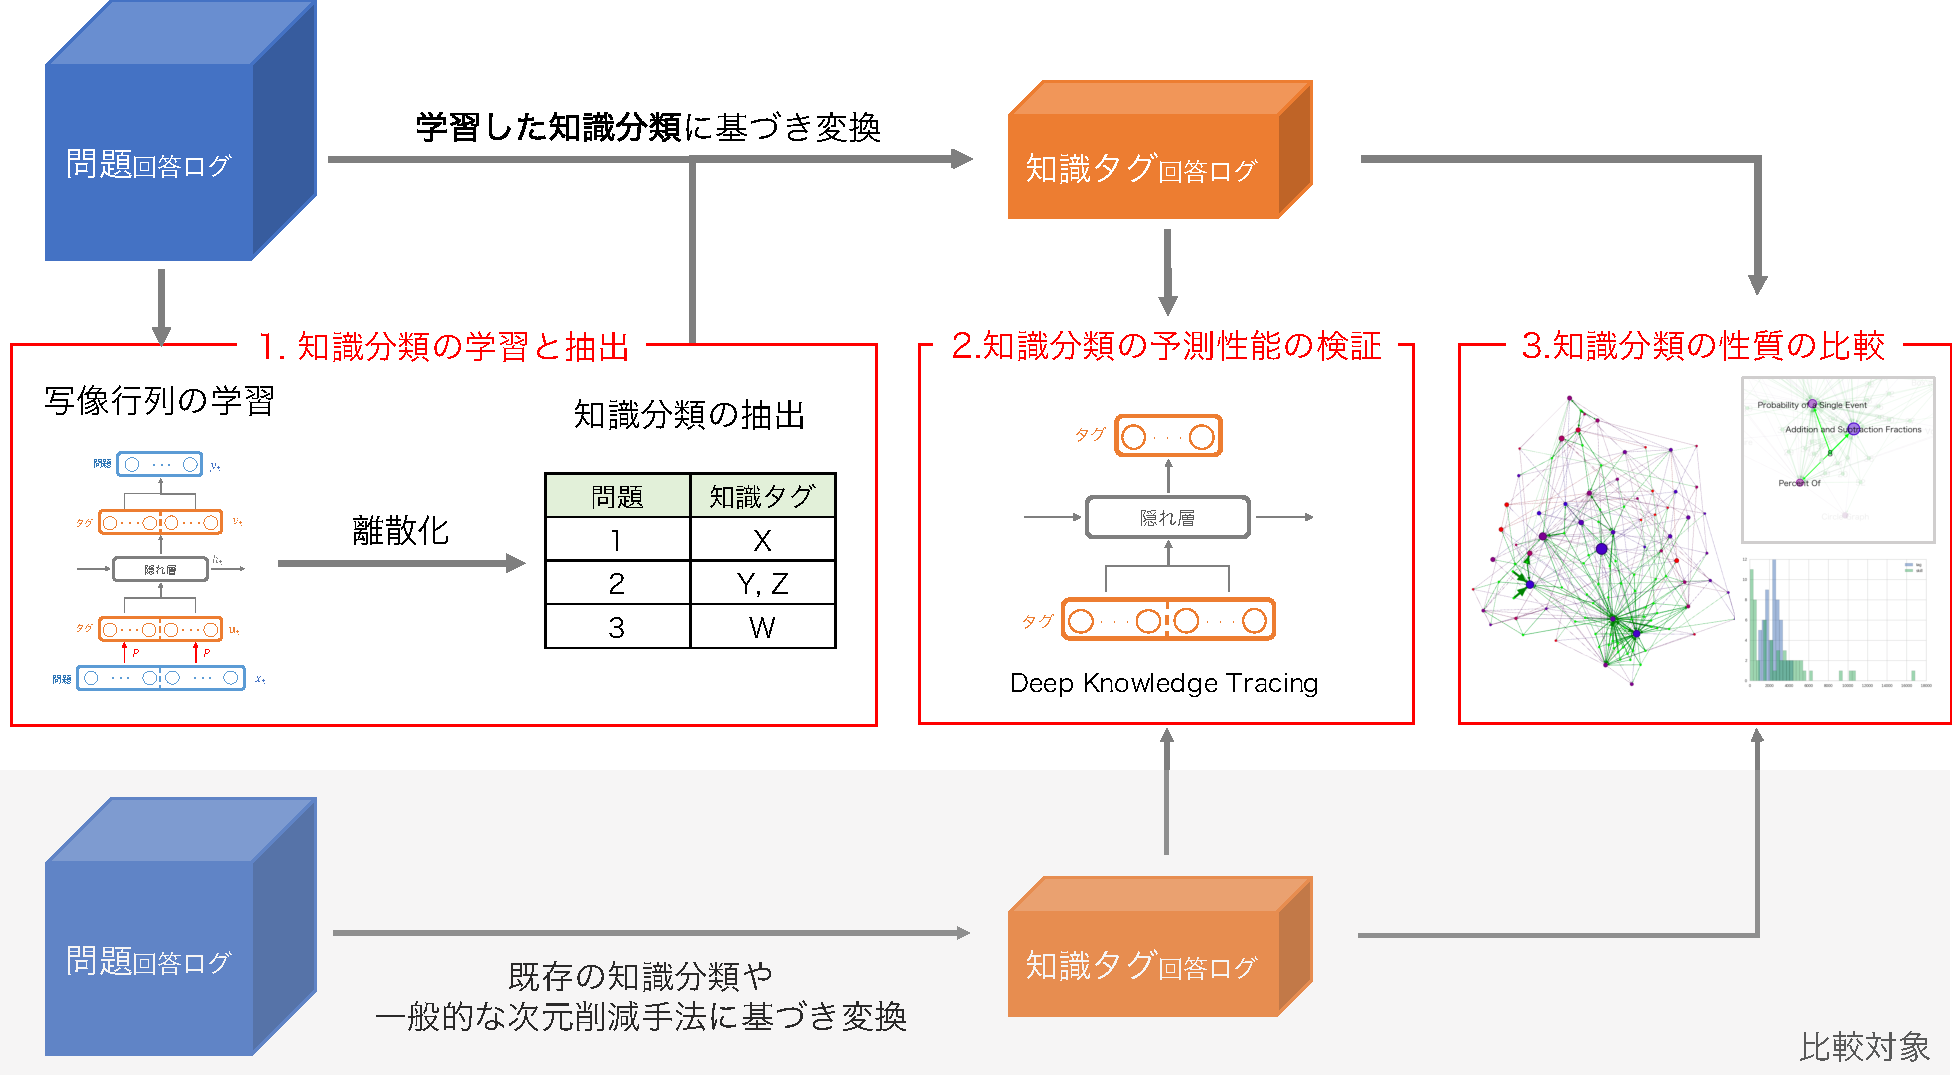
\includegraphics[width=400pt]{./img/workflow4.pdf}
\end{center}
%\caption{分析手法の流れ \newline\small 網掛け部は提案手法の比較対象となる手法を表す.}
\caption{分析手法の流れ}
\label{fig:workflow}
\end{figure}

以降では,
データセットの作成,
知識分類の学習と抽出,
知識分類の予測性能の検証,
知識分類の性質の比較
について順に詳述する.


\section{データセットの作成}
本研究においては,
生徒の問題回答ログデータをデータセットとして用いる.
生徒の問題への回答結果は,その問題が問う知識を,生徒が既に獲得しているか否かを表現していると捉えることができるため,
回答結果が正解であれば,該当の知識を既に獲得しており,
回答結果が不正解であれば,該当の知識を未だ獲得していないと捉えることができるからである.

問題回答ログデータから作成するデータセットは,下記の要件を満たす必要がある.
\begin{enumerate}
	\item データセットが大規模であること.
	\item 比較検証できるデータセットが複数存在すること.
	\item 既存の知識分類が存在すること.
\end{enumerate}


まず,データセットが大規模である必要について説明する.
一般に,深層学習は大量のデータを元に特徴的な表現を抽出するため,
深層学習モデルを十分に学習させるには大規模なデータが必要であり,
これは,本研究で用いる,Recurrent Neural Networks(RNN)を活用するDeep Knowledge Tracingについても同様である\cite{piech2015deep}.
したがって,大規模なデータを有することがデータセットの要件の一つとなる.
また,深層学習によって知識獲得の予測を行う本研究においては,単に全体のデータ数が多いだけでなく,
分析対象となる個別の問題や生徒について,十分なデータ数を確保できることが重要である.
例えば,一度しか回答されていない問題については,
その問題の正答や誤答によって生徒の知識状態がどのように変化するかが観察できないため,分析に適していない.
また,十分な数の生徒のデータがないと,特定の生徒の学習傾向が強く反映され,
実験結果の一般性が損なわれる可能性がある.


次に,比較検証できるデータセットが複数存在する必要について説明する.
本研究で用いる,問題回答ログからなるデータセットは,
そのデータセットが提供されるプラットフォームにより,問題を回答している集団や,扱っている教科,内容のレベルなどが異なる.
特定のデータセットのみに対して得られた結果は,そのデータセットの環境においてのみ有効である可能性があり,
一般性のある結果や知見が得られたとは言いにくい.
そのため,本研究では,教科を数学に絞った上で,複数のプラットフォームにおける問題回答ログから作成された複数のデータセットを用いることで,
手法の一般性を検証する.
なお,数学に限らない,他教科への適用可能性については,第6章で考察する.


最後に,既存の知識分類が存在する必要について説明する.
本研究では.現在の一般的な知識獲得予測に用いられている知識分類は,
人間の複雑な知識獲得の過程を表現する上で最適化された表現ではない,という仮定に立ち,
問題回答ログのみを利用して,より最適化された知識分類を抽出することを目的としている.
抽出された知識分類の妥当性を検証するには,既存の知識分類と比較することが必要であり,
そのため,分析対象となるデータセットは,既存の知識分類を有する必要がある.





\section{知識分類の学習と抽出}
\label{sec:main}
本節では,提案手法による知識分類の学習と抽出について述べる.
本研究では,
知識獲得予測を最適化する知識分類を学習するために,
問題空間を知識タグ空間に変換する写像行列をパラメータ化し,知識獲得予測の最適化の過程で同時に学習する.
なお,以降では,この提案手法のモデルを「知識分類学習モデル」と呼ぶ.
この知識分類学習モデルの構造は,Deep Knowledge Tracing(以下,DKT)を元に設計されているため,
まず,DKTを拡張する方法について述べる.

%その後,抽出された問題空間を知識タグ空間に写像する関数を離散化し,実際の知識分類を作成する方法について述べる.


\subsection{DKTの拡張による写像行列の学習}
\label{sec:tag_learn}

問題空間を知識タグ空間に変換する写像行列をパラメータ化し,Knoeledge Tracingの最適化の過程で同時に学習するために,
本研究では,既存のDKTの構造を拡張した「知識分類学習モデル」を設計する.
DKTのモデルを拡張する方法を,以下の3つの要素に分けて説明する.

\begin{enumerate}
	\item 入力データの粒度
	\item モデル全体の構造
	\item 最適化手法
\end{enumerate}


\subsubsection{入力データの粒度}
まず,既存のDKTと大きく異なる点として,モデルに入力されるデータの粒度の違いについて述べる.

DKTのモデルにおいては,使用するデータセットは生徒の問題回答ログデータであるが,
モデルへの入力は,事前に定義された知識分類に基づいて,知識タグに落とし込まれ,どの知識タグが紐づく問題に回答したかが入力される.
これは,既存の知識分類の範囲内で生徒がどのように知識を獲得していくかを予測することを前提にしているためであるが,
本研究においては,そもそもの問題と知識分類の関係性を最適化することを目的とするため,このような入力は適さない.
よって本研究では,モデルへの入力は問題に対する回答のままにとどめ,
生徒が次にどの問題に正解するかを予測する過程において,
深層学習モデル自身に最適な知識分類方法を判断させ,学習させる.
こうして学習された知識分類は,結果的に知識獲得の文脈で最適化されている可能性が高く,
既存の知識分類と比較することで,その性能や性質を解釈することができる.


\subsubsection{モデル全体の構造}
次に,具体的なモデル全体の構造の拡張について述べる.

\begin{figure}[htb]
\begin{center}
	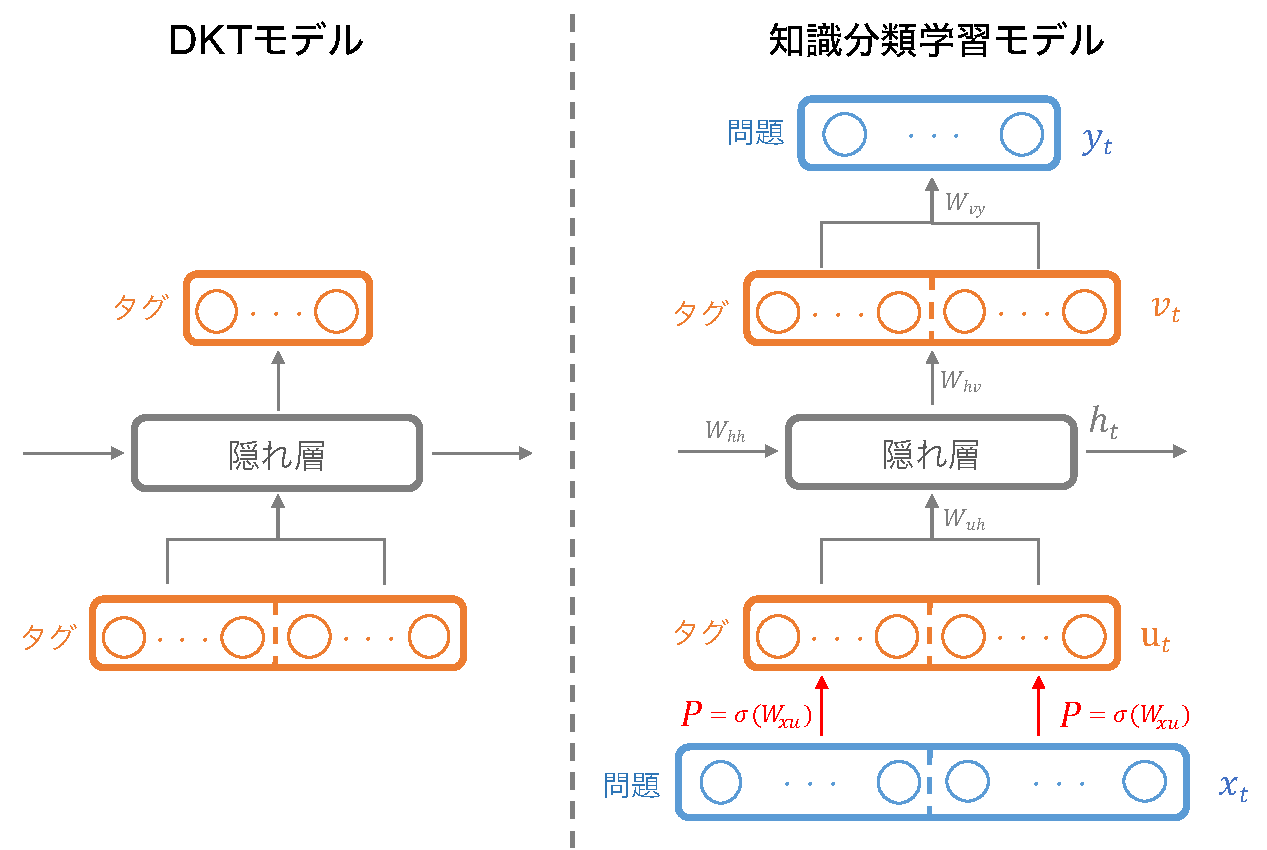
\includegraphics[width=360pt]{./img/model.pdf}
	\caption{モデル構造上の拡張}
	%\caption{モデル構造上の拡張 \protect \footenotemark}
	\label{fig:model}
\end{center}
\end{figure}

まず,
DKTでは入力が隠れ層へ直接伝達されるのに対し,
知識分類学習モデルは,
まず入力層の問題空間から,抽出目的の知識タグ空間への写像を行う.
ここで言う知識タグ空間とは,既存の知識分類と同じ次元数に設定された空間で,
問題回答の正誤の情報を低次元の空間で表すことを目的としている.

具体的には,
まず,問題数を$M$とした場合,正答と誤答を区別するため,モデルへの入力ベクトル${\bf x}_t$の長さは$2M$となる.
第二層の知識タグ空間の次元数は,既存の知識分類と同じ次元数に揃え,事前に$N$と定義する.
そして,$M$次元の問題空間から$N$次元の知識タグ空間へ変換する写像行列${\bf P}$を,以下の式により定義する.
\begin{eqnarray}
\label{eq:p}
%{\bf P({\bf x})} = \sigma( {\bf W}_{xu} {\bf x} + {\bf b}_u)
{\bf P} = \sigma( {\bf W}_{xu})
\end{eqnarray}
ここで,
%${\bf x}$は長さ$M$の問題空間ベクトルを指し,
${\bf W}_{xu}$は$M \times N$の大きさの重み行列を指し,
%${\bf b}_u$は長さ$N$のバイアス項を指し,
$\sigma$はシグモイド関数を指す.
%訓練時には,${\bf W}_{xu}$,${\bf b}_u$を学習する.
訓練時には${\bf W}_{xu}$を学習する.

このように定義される写像行列${\bf P}$を,${\bf x}_t$の前半の正答部分と後半の誤答部分に別々に適用し,連結することによって,
正誤の情報を区別したまま,
長さ$2N$の知識タグ空間ベクトル${\bf u}_t$が生成できる.
\begin{eqnarray}
{\bf x}_t &=& [{\bf x}_{t\_positive}, {\bf x}_{t\_negative}]\\
%{\bf u}_t &=& [{\bf P}({\bf x}_{t\_positive}), {\bf P}({\bf x}_{t\_negative})]
{\bf u}_t &=& [{\bf P} {\bf x}_{t\_positive}, {\bf P} {\bf x}_{t\_negative}]
\end{eqnarray}
ここで,${\bf x}_{t\_positive}$,${\bf x}_{t\_negative}$はそれぞれ問題回答の正答と誤答を表す長さ$M$のベクトルである.

こうして得られた知識タグ空間ベクトル${\bf u}_t$は,
一般的なRNN同様,隠れ層を経由して時系列情報を反映した後,再び長さ$2N$の知識タグ空間ベクトル${\bf v}_t$となる.
\begin{eqnarray}
%{\bf h}_t &=& \tanh({\bf W}_{uh} {\bf u}_t + {\bf W}_{hh}  {\bf h}_{t-1} + {\bf b}_h)\\
{\bf h}_t &=& \varphi({\bf u}_t, {\bf h}_{t-1}, {\bf \theta})\\
{\bf v}_t &=& \sigma( {\bf W}_{hv} {\bf h}_t + {\bf b}_v)
\end{eqnarray}
ここで,
${\bf h}_t$は時刻$t$の隠れ層を指し,
${\bf W}_{hv}$は重み行列を指し,
${\bf b}_v$はバイアス項を指し,
$\varphi$は活性化関数を表す.
なお,${\bf \theta}$は任意のパラメータを指し,用いる活性化関数によって異なる.
訓練時には${\bf \theta}$,${\bf W}_{hv}$,${\bf b}_v$を学習する.
この知識タグ空間ベクトル${\bf v}_t$は,時刻$t$までの回答情報を反映した,生徒の知識タグ空間における知識状態を表しているといえる.

最終的に,この知識タグ空間ベクトル${\bf v}_t$から,$M$次元の問題回答予測ベクトル${\bf y}_t$を算出する.
\begin{eqnarray}
{\bf y}_t &=& \sigma( {\bf W}_{vy} {\bf v}_t + {\bf b}_y)
\end{eqnarray}
ここで,
${\bf W}_{vy}$は重み行列を指し,
${\bf b}_y$はバイアス項を指す.
学習時には${\bf W}_{vy}$,${\bf b}_y$を学習する.

${\bf y}_t$は0から1の間の値を取り,次の時刻$t+1$において各問題に正答する確率を表しており,
既存のDKTと同様の予測表現となっている.


以上のようなモデル構造上の拡張をまとめた図を図\ref{fig:model}に表す.
橙色の層は知識タグ空間を,青色の層は問題空間を表し,層が左右で二つに区切られている部分は前半・後半がそれぞれ正答・誤答の情報を表現している.
%問題空間から知識タグ空間への写像行列${\bf P}$は${\bf P}=\sigma({\bf W} x + b)$で表され.正答部分と誤答部分に同じ関数が適用される.
この拡張の目的は,
$M$次元の問題空間を$N$次元の知識タグ空間へ変換する写像行列${\bf P}$をパラメータ化し,
知識獲得予測の最適化を行う過程で学習することにある.



\subsubsection{最適化手法}
最後に,最適化手法の拡張について述べる.

既存のDKTにおける最適化手法は,
時刻$t$の出力である問題回答予測ベクトル${\bf y}_t$と,実際の時刻$t+1$の問題回答ベクトル${\bf\tilde{ \delta}}({\bf q}_{t+1})$の誤差を損失関数として,これを最小化するものである.
${\bf a}_{t+1}$を時刻$t+1$に対応する問題で正答したか否か($1$か$0$)のベクトルとすれば,
\begin{eqnarray}
\label{eq:log_sum}
{\log(p_1 \times p_2 \times \dots \times p_{m_t}) = \sum_{k}^{m_t} \log(p_k)}
\end{eqnarray}
であることから,損失関数は
\begin{eqnarray}
\label{eq:prediction_entropy}
{L_p = \sum_t l({\bf y}_t^T {\bf \tilde{\delta}}({\bf q}_{t+1}), {\bf a}_{t+1})}
\end{eqnarray}
である.
この損失関数を,回答正誤予測に関する損失関数$L_p$とする.


本研究では,この回答正誤予測に関する損失関数に加え,2種類の損失関数を導入する.

まず一つ目の損失関数は,
式\ref{eq:autoencoder_hidden}--\ref{eq:autoencoder_loss}で表される再構成誤差である.
ここで,式\ref{eq:autoencoder_hidden},\ref{eq:autoencoder_reconstruct}におけるパラメータについては,
本研究では,
${\bf W}$,${\bf b}$が,
入力層で問題空間から知識タグ空間へ写像する際に用いる
${\bf W_{xu}}$,${\bf b_u}$
であり,
${\bf W'}$,${\bf b'}$が,
出力層で知識タグ空間から問題空間へ写像する際に用いる
${\bf W_{vy}}$,${\bf b_y}$
である.
この損失関数を,再構成誤差$L_p$とする.

再構成誤差を損失関数に導入する理由について述べる.
まず,一般的に再構成誤差を用いるAutoencoderは,
深層学習モデルに良い初期値を与えるための事前学習のための仕組みとして用いられるが,
本研究では,このAutoencoderの構造を回答正誤予測と同時に学習させるようにモデルに組み込んでいる.
Autoencoderの構造を,事前学習ではなく普通の学習モデルに組み込むことは,
必ずしも精度向上につながるわけではないため一般的ではなく,
通常は単純に低次元ベクトルへの埋め込み(Embedding)のみに留まることが多い.
本研究では,
一部,深層学習によって知識分類を学習するには十分とはいえないログ数の問題が存在しており,
データの特徴を把握しきれない未学習(underfitting)の状況に陥る可能性があることを確認した.
そうした学習不足への対策として,モデルの学習を矯正し,適切に学習を進めさせる正則化項として再構成誤差を導入している.
このように,データ数が不足する場合に,モデルがより適切に学習を進めるように様々な正則化項を設ける手法は一般的であり,
有効な手法とされている.
学習される知識分類の性質への影響についても検討した結果,
Autoencoderの構造は,
問題の正答・誤答と知識タグの理解状態は相互に変換できるはずだという
教育学的な文脈との整合性と合致し,知識分類の性質を損ねないと判断したため,適用している.


もう一つの誤差関数は,以下の式で表されるもので,これを以下「スパース正則化項」と呼ぶ.
\begin{eqnarray}
\label{eq:sparse}
L_s = {1\over n}\sum_{i=1}^n (0.5 - |{\bf u}_i - 0.5|)
\end{eqnarray}
ここで,${\bf u}_i$はユーザ$i$の回答についての第二層の知識タグ空間ベクトルである.
この損失関数を,スパース正則化項$L_s$とする.

スパース正則化項を損失関数に導入する理由について述べる.
本研究においては,離散表現のタグとしての知識分類を抽出するため,知識分類学習モデルによって学習された写像行列$P$をなんらかの手段によって離散化する必要がある.
離散化の方法は様々であるが,いずれの方法をとっても,0から1の値を取る連続表現が0か1の2値を取る離散表現になることにより,情報量の損失が避けられない.
知識分類学習モデルによって学習された写像行列の情報量をできるだけ保ったまま離散化を行うには,初めから写像行列が離散表現に近い形式になっていることが望ましい.
式\ref{eq:sparse}では,$L_s$は${\bf u}_i$の各値が0.5に近いほど大きく,0か1に近いほど小さくなるように設計されているため,
最適化の過程で自動的に離散表現に近い写像行列が得られるようになっている.


結果的に,
モデル全体の損失関数$L$は以下の式によって定められ,
この損失関数を最小化するようにモデルが最適化される.
\begin{eqnarray}
\label{eq:total_loss}
{L = L_p + L_r + L_s}
\end{eqnarray}


\subsection{写像行列の離散化による知識分類の抽出}
\ref{sec:tag_learn}項の知識分類学習モデルで得られた写像行列${\bf P}$から,
実際に知識分類を作成し,既存の知識分類と比較する手法について説明する.


知識獲得予測の最適化の過程で得られた写像行列${\bf P}$は,
$M$次元の問題空間を$N$次元の知識タグ空間に写像する$M \times N$の大きさの行列として表現されている.
この行列は0から1の値を取る連続値表現であるため,そのままでは問題がどの知識タグに紐づくかを特定することはできない.
そのため,何らかの方法で,この行列を0か1の2値を取る離散表現に改める必要がある.

離散化の方法としては,各問題において最も値の大きい要素のみを1とする方法や,
行列全体で特定の閾値を定め,その閾値を超えた要素を1とする方法,
両者を組み合わせる方法など,
様々な方法が考えられる.
%各方法によって,抽出された知識タグの性質の異なる解釈をすることが可能だが,
本研究では,知識獲得予測に適用した際に最も良い精度で予測できる分類を,
知識獲得の過程を最もよく説明する分類として見なして利用し,その性質も解釈する.
まず,
各手法において得られた写像行列を,以下の条件に基づいて離散化し,
DKTにおいて最も高い精度を発揮したものをその手法による精度の上界として採用する.
\begin{enumerate}
\item 各問題の写像ベクトルにおいて,最も値が大きい要素を1とする
\item 写像行列全体において,値が閾値$Y$以上の要素を1とする
\item 写像行列全体において,1でない要素を0にする
\end{enumerate}


\section{知識分類の予測性能の検証}
次に,
抽出された知識分類の知識獲得予測における性能を検証する手法について述べる.
本研究では知識獲得の予測性において最適化された知識分類を,深層学習によって抽出できることを示すことを目的としている.
そのため,\ref{sec:main}項で抽出された知識分類を用いて知識獲得予測を行った際に,
既存の知識分類を用いる場合よりも高い精度で予測が行えることを示す必要がある.


まず,既存の知識分類(以下,既存タグ)を用いてDKTによって知識獲得予測を行った場合の精度をベースラインとして定める.
次に,抽出された知識分類(以下,抽出タグ)を用いてDKTによって知識獲得予測を行い,その精度をベースラインと比較する.
知識獲得予測のタスクは,
生徒の時刻$t$において観測された問題回答結果を$q_{t}$として,
$q_1, q_2, \dots, q_t$から$q_{t+1}$の正誤確率を求めるというものであるため,
各問題を既存タグないしは抽出タグに紐付けて,
$q_{t}$をタグに対する回答と見なしてモデルに入力することで,タグ同士の性能の比較が可能になる.

また,この精度向上が,知識獲得予測の最適化の過程で知識分類を作成したことに起因することを示すため,
知識獲得予測と無関係の,一般的な事前学習のAutoencoderで作成した知識タグを用いた場合とも比較を行う.
これは,本手法による知識分類の作成が,
\begin{itemize}
	\item 人間の可読性を目的として人間によって設計された分類か否か
	\item 知識獲得予測の文脈で最適化された分類か否か
\end{itemize}
という二つの観点において新規性を有することを受け,
性能の変化が何に起因してもたらされたのかという,差分をより明確にするために行う検証である.




\section{知識分類の性質の比較}
最後に,
抽出タグの性質について,既存タグとの比較を通して,定量的・定性的な分析を行う.
これは,本手法によって知識獲得予測の精度が向上するという検証だけでなく,
知識獲得予測において最適化されている知識分類の性質を解釈し,知見を得ることで,
教育における実用性を考察することにつなげることが目的である.

まず,定量的な分析として,
抽出タグと既存タグの各タグが回答ログに出現する回数の分布に着目する.
抽出タグと既存タグはそれぞれ異なる基準で作成されており,問題との紐付き方が異なる.
そのため,問題をタグに変換した場合に,抽出タグと既存タグで,回答ログにおける出現回数,
すなわちモデルに入力される回数の分布が異なる可能性が高い.
モデルの入力の分布の違いは予測精度に直接的に影響を与える可能性が高く,
この分布を分析することで,
知識獲得予測の精度を向上させる要因を,データ構造という側面から分析する.

また,定性的な分析として,
抽出タグと既存タグが内容の面においてどのような関係性があり,
抽出タグがどのような問題をカバーするタグとなっているのかに着目する.
%抽出タグによって既存タグがどのように再配置されたのかを検証する.

抽出タグと既存タグの内容を比較する方法として,まず,
抽出タグが紐づく問題と,既存タグが紐づく問題から,抽出タグと既存タグの共起行列を作成する.
この行列は,各抽出タグと既存タグとの関係性の近さを表現した行列と捉えることができるが,
各抽出タグの内容的特徴をより明確に捉えるために,既存タグごとに最大値で割って正規化した行列を作成し,
この行列をタグ関係行列とする.

%TF-IDF法を用いて,特徴の重み付けを行う.
%TF-IDF法は,元々文書の分類に用いられる手法で,
%複数の文書がある時に,各文書を特徴づける単語を特定することを目的にしている.
%具体的には,まず,各文書内での,各単語の出現頻度(Term Frequency,以下$TF$)を求める.
%$TF$は,文書内に多く出現する単語ほど重要だ,という考えに基づいた指標であるが,
%$TF$のみだと,例えば助詞や助動詞といった,いくつもの文書で横断的に使われている単語の重要度が高くなってしまうため,
%各単語が全文書の内いくつの文書に現れているかという制約(Inverse Document Frequency,以下$IDF$)を設けて,
%一般的な単語の影響を除外する.
%単語$i$の文書$j$における$TF_{i,j}$,単語$i$の$IDF_i$と,それらを用いたTF-IDF値($TFIDF_{i,j}$)は以下の式で表される.
%\begin{eqnarray}
%TF_{i,j} &=& \frac {n_{i,j}}{\sum _{k}n_{k,j}}
%\\
%IDF_i &=& \log {\frac {|D|}{|\{d:d\ni t_{i}\}|}}
%\\
%TFIDF_{i,j} &=& TF_{i,j} \cdot IDF_i
%\end{eqnarray}
%$n_{i,j}$は単語$i$の文書$j$における出現回数を指し,
%$\sum _{k}n_{k,j}$は文書$j$におけるすべての単語の出現回数の和を指し,
%$|D|$は総文書数を指し,
%$|\{d:d\ni t_{i}\}|$は単語$i$を含む文書数を指す.
%
%
%さて,今回の抽出タグの特徴付けにおいては,各既存タグが単語にあたり,抽出タグ1つ1つが文書にあたる.
%複数の抽出タグに共通して現れる既存タグほど,特徴づけにおける重みが小さくなり,
%特定の抽出タグのみに現れる既存タグほど,特徴づけにおける重みが大きくなる.
%この手法により各抽出タグの特徴付けを行い,各抽出タグにおいて特徴的な既存タグを強調した共起行列(以下,タグ関係行列)を作成する.

次に,既存タグをノードとする知識間影響ネットワーク(以下,既存タグネットワーク)を,\ref{sec:dkt}項で述べた既存のDKTで用いられた手法に基づいて作成しする.
この既存タグネットワークの各ノード(既存タグ)に対し,タグ関係行列を元に抽出タグのノードを紐付けることで,両タグの関係性を表すネットワーク(以下,タグ関係ネットワーク)を作成する.
こうして得られたタグ関係ネットワークを用いることで,既存タグを知識間の影響に基づいて配置した上で,抽出タグとの関係性を俯瞰することが可能であり,このネットワークを元に両タグの構造や内容的な関係性を考察する.

以上の処理の流れを図\ref{fig:networkflow}にまとめた.

\begin{figure}[htb]
\begin{center}
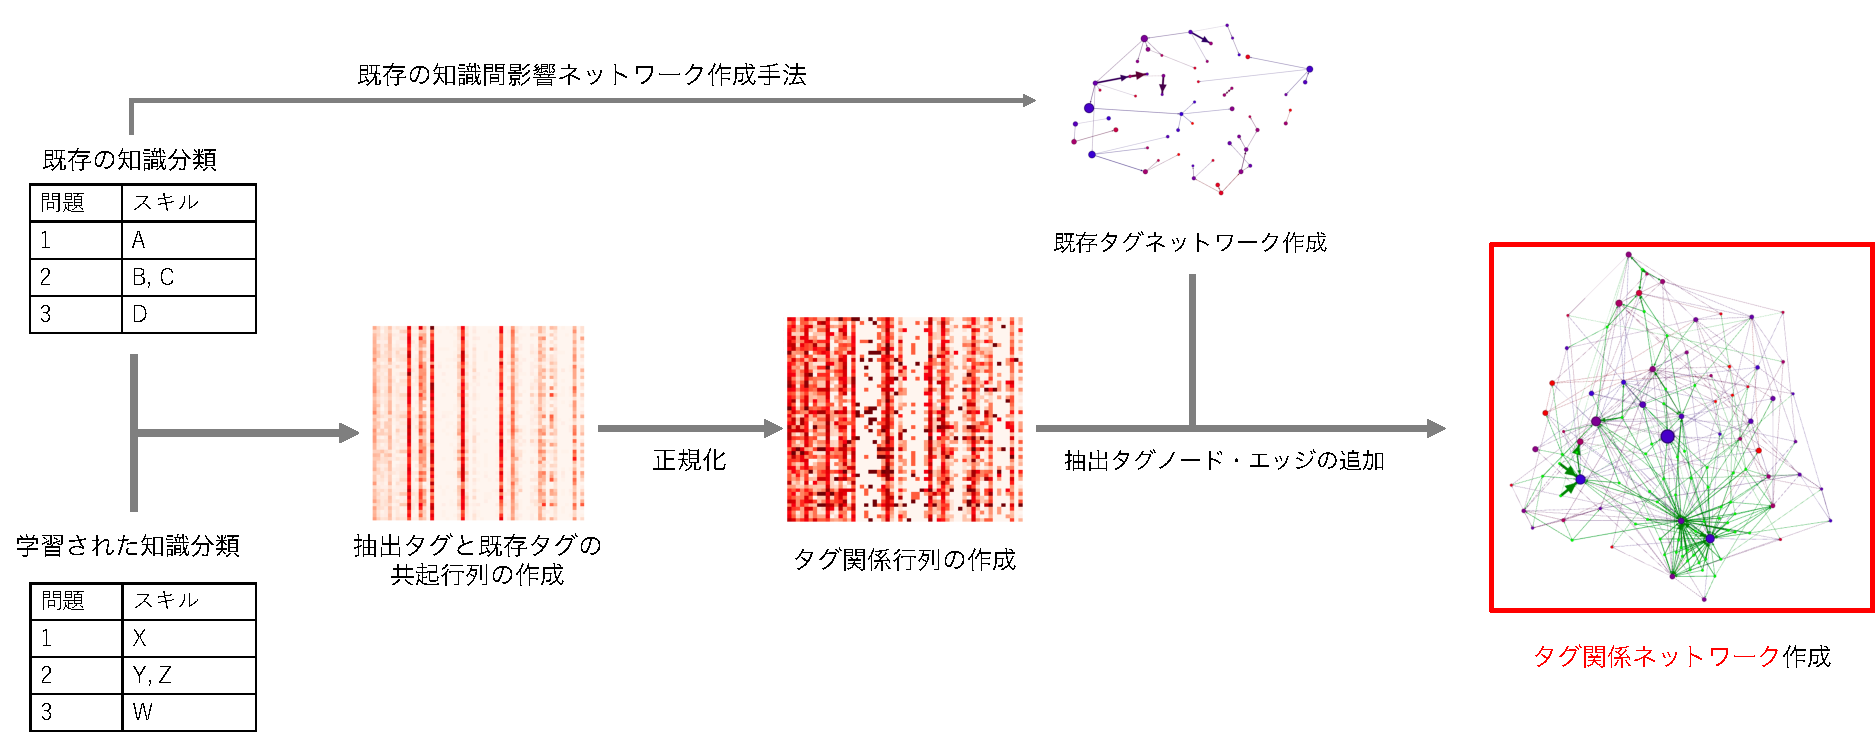
\includegraphics[width=400pt]{./img/networkflow2.pdf}
\end{center}
\caption{ネットワーク作成の流れ}
\label{fig:networkflow}
\end{figure}



\chapter{データセット}
\label{chap:dataset}
\fancyhf{}
\rhead{\thepage}
\lhead{第\ref{chap:dataset}章 データセット}
\cfoot{\thepage}


本章では,
実験で用いるデータセットについて述べる.
データセットは,小学4年生から中学3年生を対象とする国内最大級のMOOCs「勉強サプリ\footnote{\url{https://benkyosapuri.jp/}}」で提供される11の講座の問題回答ログデータから作成する
\footnote{本論文の研究は勉強サプリを運営するリクルートマーケティングパートナーズ(株)との共同研究プロジェクトの一環で行われている.}
.
まず,勉強サプリから収集されたログデータが分析に利用するためのデータ要件を満たした本分析に最適なデータであることを述べる.
次に,実験で用いる宣言的知識の獲得を主目的とするデータセットと手続き的知識の獲得を主目的とするデータセットの作成について述べる.
特に,
歴史や地理に関する講座の問題が主に宣言的知識の獲得の有無を評価する問題であることを指摘し,
歴史や地理に関する5講座から宣言的知識の獲得を主目的とするデータセットとして5つのデータセットを作成する.
また,
算数や数学に関する講座の問題が主に手続き的知識の獲得の有無を評価する問題であることを指摘し,
算数や数学に関する6講座から手続き的知識の獲得を主目的とするデータセットとして6つのデータセットを作成する.






\section{勉強サプリ}
ここでは,勉強サプリより収集された問題回答ログデータが本分析に最適なデータであることを述べるため,
まず,勉強サプリについて説明する.
% - 勉強サプリは5W1H(what, who, when, where, why, how)
勉強サプリは主に小学4年生から中学3年生を対象とした国内最大級の大規模オンライン講座である.
リクルートマーケティングパートナーズ(株)が運営している.
サービスは2015年に開始された.
学習者はオンライン上で問題回答形式によるドリル演習や
動画視聴形式による授業聴講を通して勉強する.
小学生には各学年ごとに国語,社会,算数,理科の4科目が,
中学生には各学年ごとに国語,数学,英語の3科目と 
学年共通で地理,歴史,公民,理科1,理科2の5科目が提供されており
合計26の講座が提供されている.
%フリーミアム形式で提供されており,
無料で利用できるコンテンツもある.



% - 統計量
勉強サプリは提供教材,利用者数,学習行動ログ数の点でサービスの規模が非常に大きい.
4,000以上の授業動画と7,000近い演習問題を提供しており,
サービス開始から1年経たずして,
利用者は5万人以上おり,
講義視聴ログ数は100万以上,
問題回答ログ数は総計で1,000万以上である\footnote{2015年11月31日時点.}.


% - 利用画面
\begin{figure}[!htb]
\begin{center}
	\hspace*{-10pt}\makebox[1.2\textwidth][c]{
		\minipage{0.52\textwidth}
			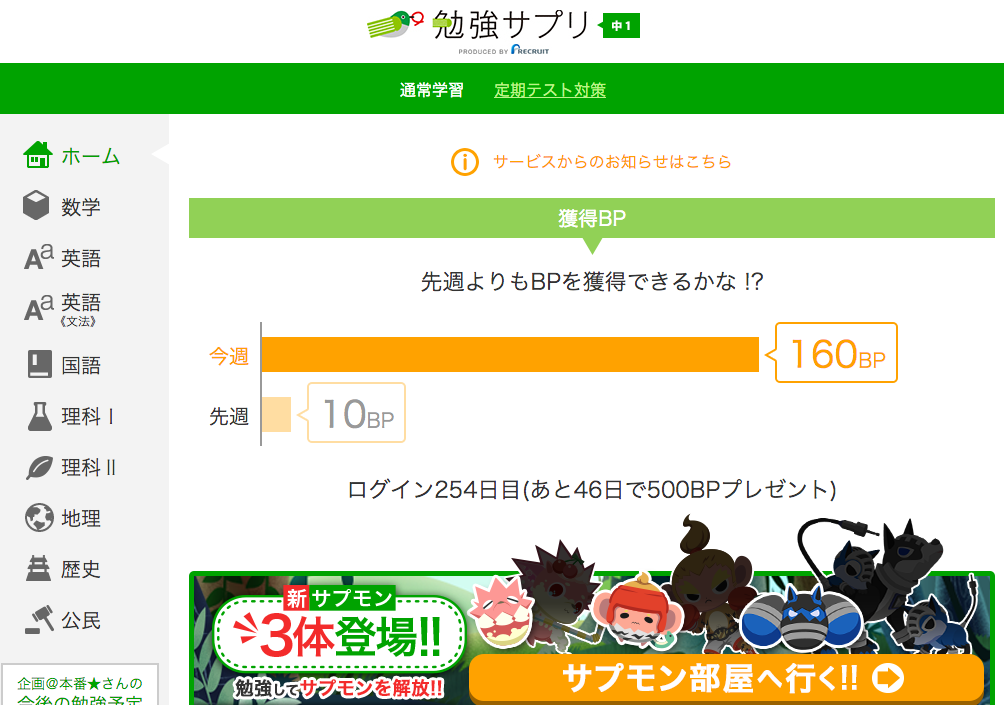
\includegraphics[width=200pt, height=160pt]{./img/benkyo1.png}
			\caption{勉強サプリのマイページ}
			\label{fig:benkyo1}
		\endminipage\hfill
		\minipage{0.52\textwidth}
			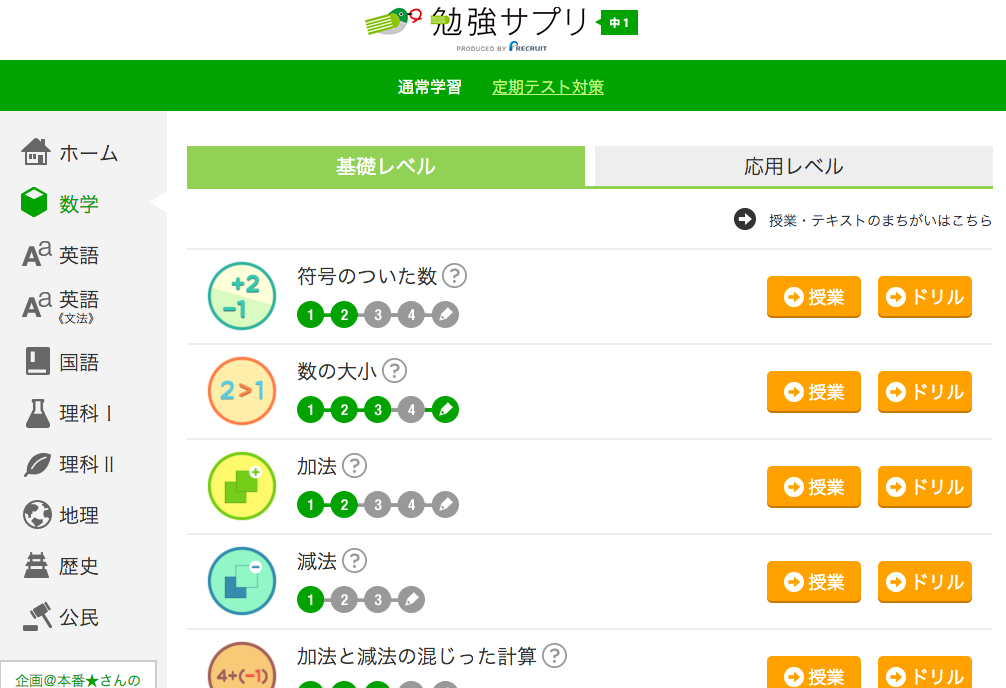
\includegraphics[width=200pt, height=160pt]{./img/benkyo2.png}
			\caption{勉強サプリの講義一覧ページ}
			\label{fig:benkyo2}
		\endminipage\hfill
	}
	\hspace*{-10pt}\makebox[1.2\textwidth][c]{
		\minipage{0.52\textwidth}
			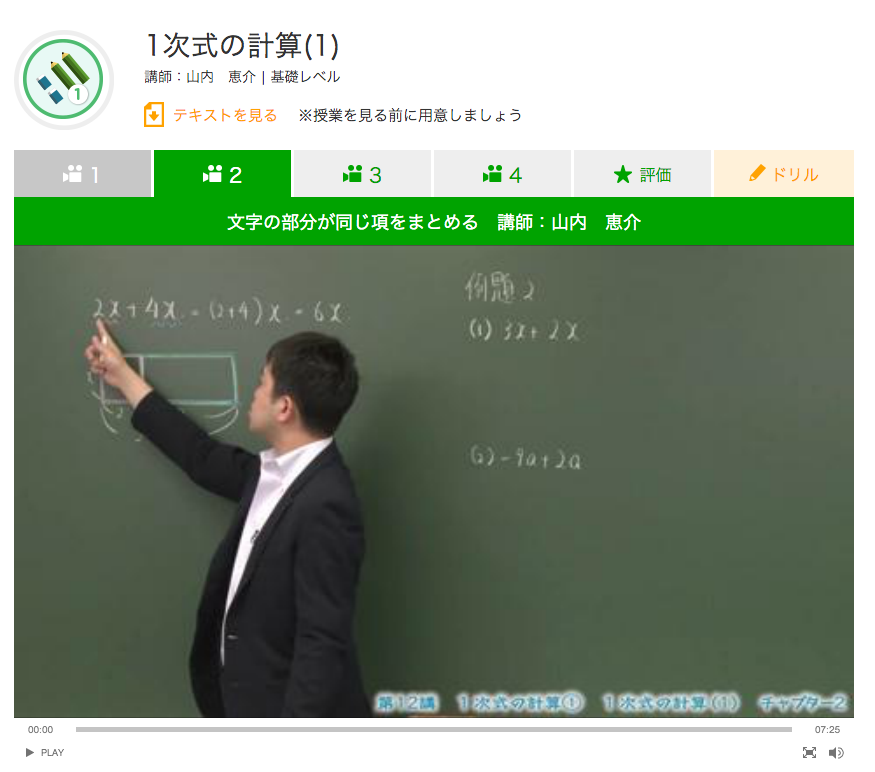
\includegraphics[width=200pt, height=160pt]{./img/benkyo3.png}
			\caption{勉強サプリの講義視聴ページ}
			\label{fig:benkyo3}
		\endminipage\hfill
		\minipage{0.52\textwidth}
			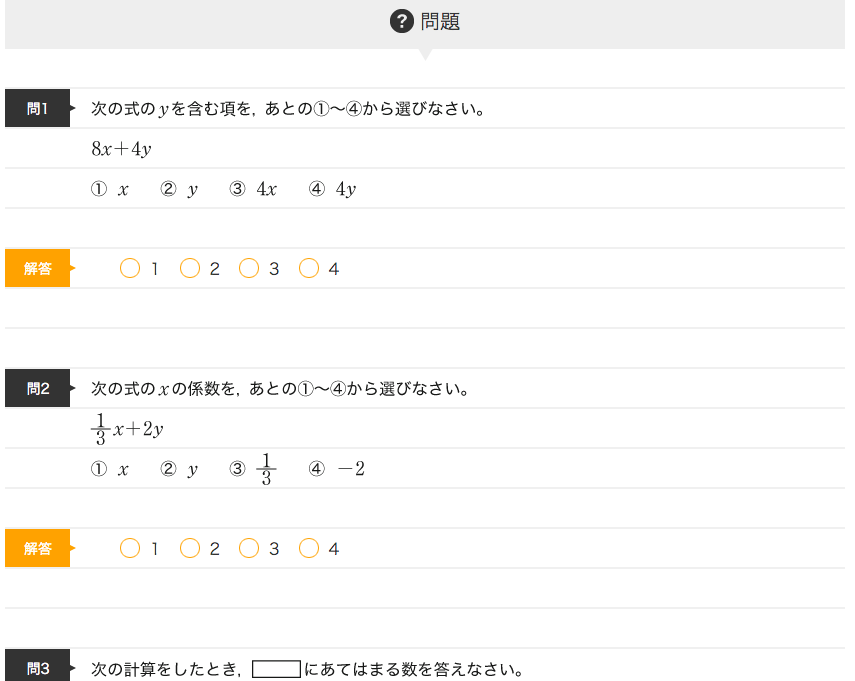
\includegraphics[width=200pt, height=200pt]{./img/benkyo4.png}
			\caption{勉強サプリの問題演習ページ}
			\label{fig:benkyo4}
		\endminipage\hfill
	}
\end{center}
\end{figure}
サービスの具体を利用画面を交えて説明する.
図\ref{fig:benkyo1},\ref{fig:benkyo2},\ref{fig:benkyo3},\ref{fig:benkyo4}にページのイメージを記載する.
図\ref{fig:benkyo1}はログイン後のマイページを示している.
学習に関するコンテンツだけでなく,
利用継続性の向上を狙って,ポイントというシステムやサプモン(勉強サプリのモンスター)というアバターを用いたゲームを大きく表示している.
図\ref{fig:benkyo2}は中学1年向け数学の講義一覧ページを示している.
ユーザは講義視聴のドリル演習の両方あるいはどちらかを勉強できる.
図\ref{fig:benkyo3}は講義視聴ページを示している.
講義視聴ページは視聴しやすいように細かく分割されている.
図\ref{fig:benkyo4}は問題演習ページを示している.
問題演習はテスト形式で提供されており,一度に複数の問題が提供され,また,その採点も同時に行われる.
この問題回答から収集されるログデータの仕様は同時に1つの問題しか回答ログが入らないというDeep Knowledge Tracingで想定されている設定と異なるため,
Deep Knowledge Tracingを拡張する必要があるが,その拡張法については実験説明の際に合わせて述べる.


現在の学習指導要領\cite{gakushushidouyouryou}によると,
小学4年生の社会では社会基盤や地域社会など地理に近い内容を扱い,
小学5年生の社会では地域の山地山脈,気候など地理に近い内容を扱い,
小学6年生の社会では日本の歴史に関する内容を扱う
としており,
また,実際に,勉強サプリの学習内容も概ねそれに従っている.


勉強サプリは小学生から中学生が対象で,
その難易度は難しすぎず,
収集された問題回答ログデータは1,000万以上と膨大であり,
また,先に指摘したような地理や歴史といったいわゆる暗記系の科目と数学に関する科目が複数提供されているため,
データの要件を満足している可能性が高い.
そこで,
以降では,勉強サプリから収集された問題回答ログデータのなかで,
特に地理と歴史に関する5講座(小学4年社会,小学5年社会,小学6年社会,中学地理,中学歴史)のデータ
と,
算数や数学に関する6講座(小学4年算数,小学5年算数,小学6年算数,中学1年数学,中学2年数学,中学3年数学)のデータ
の11データよりデータセットを作成し,
これらのデータセットを
それぞれ,
宣言的知識の獲得を主目的とするデータセットと手続き的知識の獲得を主目的とするデータセットとする.


\section{データセットの作成}
データセットの作成について述べる.
データセットは問題回答ログデータから作成する.
対象期間は2015年4月から2015年11月の8ヶ月である.

勉強サプリでは学習者の回答は自動採点される.いずれの講座も回答は選択方式で,1つの回答欄には選択肢の中から1つの数字や文字を選択する.
1つの問題に複数の回答欄が存在する場合は当該問題のすべての回答欄が正解の場合に当該問題を正解した,と扱う.同時に1つの問題しか提示されないという形式だけでなく,同時に複数の問題が提示される場合もあり,その場合,採点は提示された問題群に対して同時に行われる.つまり,同時に複数の問題回答ログが発生しうるデータである.

データセットを作成する際に,前処理として回答行動ログデータから下記に該当するログデータをノイズとみなして除去した.
\begin{itemize}
	\item[条件] 同時に回答された複数の問題のログデータ群について,すべての問題の回答欄が空白で投稿されているもの.
\end{itemize}
これは,オンライン講座ではサービス上の学習者の行動には大きな制約はなく,
1クリックで簡単に問題演習ページを開けてしまえる状況にあるということや,
すべての回答欄が未記入で投稿された回答は直前に着手した問題群と同じ問題群であることが多いこと,
特に回答時間が短く誤って当該問題演習ページを開いてしまったと推察されるログが多かったからである.

以上,データセットの作成について述べた.
11データセット全体を概観する.

\section{データセットの概観}
\begin{table}[!htb]
\caption{11データセットの統計量}
\label{tab:datasets-overview}
\begin{center}
\centerline{
{
\begin{tabular}{cc|rrrrr}\hline\hline
\multirow{2}{*}{学年}&	\multirow{2}{*}{科目}	&	\multirow{2}{*}{ユーザ数}	&	\multirow{2}{*}{問題数}		&	\multirow{2}{*}{回答ログ数}		&	\multirow{2}{*}{\shortstack{回答ログ数\\ $\div$ユーザ数}}	&		\multirow{2}{*}{\shortstack{回答ログ数\\ $\div$問題数}}		\\
				&								&								&								&									&				&			\\\hline
\multirow{2}{*}{小学4年}&		社会			&	3,045						&	76							&	227,409			&	75							&	2,992	\\	
				&				算数			&	4,318						&	182							&	505,917			&	117							&	2,780	\\\hdashline	
\multirow{2}{*}{小学5年}&		社会			&	2,833						&	197							&	388,521			&	137							&	1,972	\\	
				&				算数			&	3,380						&	257							&	411,957			&	122							&	1,603	\\\hdashline	
\multirow{2}{*}{小学6年}	&	社会			&	2,891						&	202							&	434,324			&	150							&	2,150	\\	
				&				算数			&	3,225						&	245							&	395,276			&	123							&	1,613	\\\hdashline	
中学1年			&				数学			&	7,137						&	365							&	659,237			&	92							&	1,806	\\	
中学2年			&				数学			&	3,931						&	278							&	238,241			&	61							&	857	 	\\   
中学3年			&				数学			&	2,667						&	343							&	177,295			&	66							&	517	 	\\\hdashline   
\multirow{2}{*}{中学}&			地理			&	6,499						&	308							&	660,882			&	102							&	2,146	\\	
				&				歴史			&	6,381						&	364							&	853,419			&	134							&	2,345	\\	
\hline\hline
\end{tabular}
}
}
\end{center}
\end{table}
作成した11データセットを概観する.
11データセットそれぞれについてユーザ数,問題数,回答ログ数とそれらの関係性を表\ref{tab:datasets-overview}に整理した.
それぞれについて順に説明していく.

まず,ユーザ数について, 
全体として,数千以上のユーザのログデータに基づいたものとなっており,最も差の大きい2つのデータセット(中学1年の数学と中学3年の数学)間で差は$2.6$倍程度である.
特に,ユーザ数が多いのは7,000ユーザ以上の中学1年の数学で,それに続いて,6,000ユーザ以上の中学の地理,歴史である.

次に,問題数について,
全体として,数十から数百の問題に基づいたものとなっており,最も差の大きい2つのデータセット(小学4年の社会と中学1年の数学)間で差は$4.8$倍程度である.
小学生のデータセットよりは中学生のデータセットの方が問題数が大きい傾向にあり,
特に,問題数が多いのは360以上の中学1年の数学と中学歴史である.

回答ログ数については,
全体として,
数十万以上であり, 最も差の大きい2つのデータセット(中学歴史と中学3年の数学)間で差は$4.8$倍程度である.
特に回答ログ数が最も大きい中学歴史のデータセットは85万以上と大規模な問題回答ログデータからなる.

さらに,これら3つの統計量の関係性を捉えるために,ログの密度という観点からユーザ1人あたりの平均回答ログ数と問題1問あたりの回答ログ数の2つの指標を評価した.
まず,ユーザ1人あたりの平均回答ログ数について, 
全体として,数十から百数十となっており,最も差の大きい2つのデータセット(小学6年社会と中学2年数学)間で差は$2.5$倍程度である.
また,いずれのデータセットでも平均回答ログ数は問題数を下回っている.

次に,問題1問あたりの平均回答ログ数について, 
全体としては,数百から数千程度の値となっており,最も差の大きい2つのデータセット(小学4年社会と中学3年数学)間で差は$5.8$倍程度である.
特に,中学2年数学と中学3年数学が小さい傾向にある.
平均回答ログ数が最も大きい小学4年社会のデータセットは1問あたり3,000近いログデータが存在する.

以上,改めてデータセット間の各統計量について整理すると,
いずれのデータセットも非常に大規模な問題回答ログから構成されており,問題あたりのログ数という点でも十分を大きいと考えられる.
また,いずれの統計量もデータセット間においても10倍以上の開きはなく,
特に,ログ数の偏りによる今後の議論の影響は小さいと考えられる.


以上,11データセット全体を概観した.
次に,個々のデータセットを具体的に説明する.


\section{個々のデータセットの具体的説明}
本論文の対象である11データセットについて,それぞれのデータセットの性質について1つずつ述べる.
具体的には,
問題群の概要,
問題とその回答選択肢の具体例,
問題ごとの何番目に着手されるかの平均値と回答ログ数の関係
の3つである.
各問題について何番目に着手されるかの平均値は
各ユーザごとに当該講座の各問題を何番目に着手したかを算出し,
それらをユーザ全体で平均した値を用いる.
各問題について何番目に着手されるかの平均値と回答ログ数の関係を見ることで,
ユーザが講座の問題全体を均一に着手しているのか,もしくは,一部に偏っているのかを捉えることができる.
XYプロットとして可視化し,図のデータ点はそれぞれひとつの問題に相当する.

\subsubsection{小学4年社会}
\begin{figure}[ht]
\begin{center}
\minipage{0.48\textwidth}
	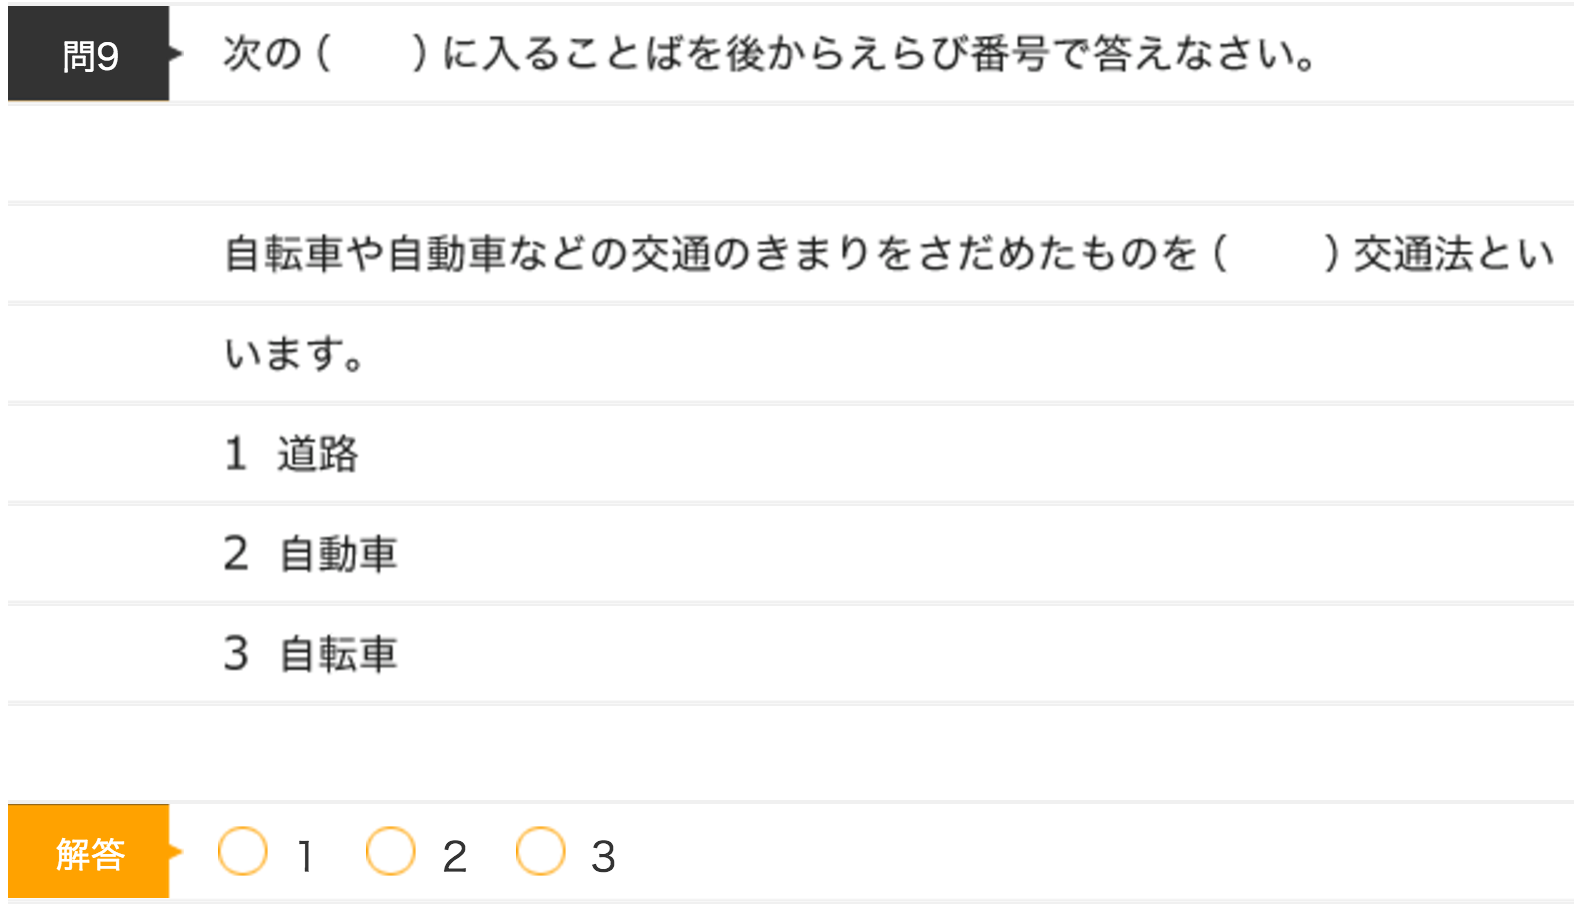
\includegraphics[width=200pt, height=150pt]{./img/qa_s4_soc.png}
	\caption{小学4年社会の問題と回答選択肢の例}
	\label{fig:qa_s4_soc}
\endminipage\hfill
\minipage{0.48\textwidth}
	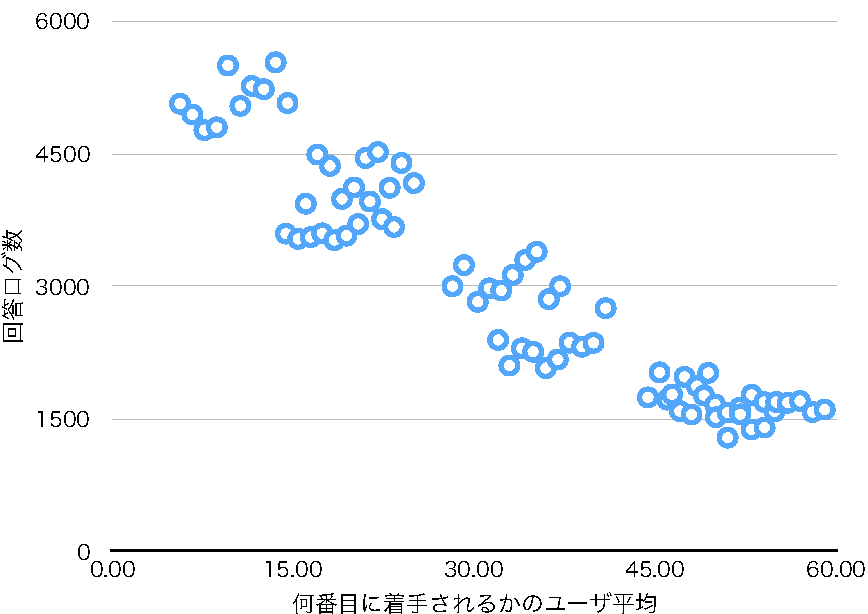
\includegraphics[width=200pt, height=150pt]{./img/stats_s4_soc.pdf}
	\caption{小学4年社会の平均着手順と回答ログ数のXYプロット}
	\label{fig:stats_s4_soc}
\endminipage\hfill
\end{center}
\end{figure}
小学4年社会では,主に,警察,消防,浄水場,ダム,汚水処理,発電所,ゴミ処理,リサイクル,水不足,地図の見方などの社会基盤や社会問題に関する基本内容が扱われる.
図\ref{fig:qa_s4_soc}に,問題と回答選択肢の例を示す.
図の問題は社会ルールのうち道路交通法に関する問題であり,
その回答を選択肢のなかから選択する,という回答形式である.
次に,各問題について何番目に着手されるかの平均値と回答ログ数の関係を図\ref{fig:stats_s4_soc}に示す.
全体として,概ね1500件以上の回答ログ数があり,最初の問題の方が回答ログが大きい傾向にあるが大きく偏っているというわけではない.



\subsubsection{小学4年算数}
\begin{figure}[ht]
\begin{center}
\minipage{0.48\textwidth}
	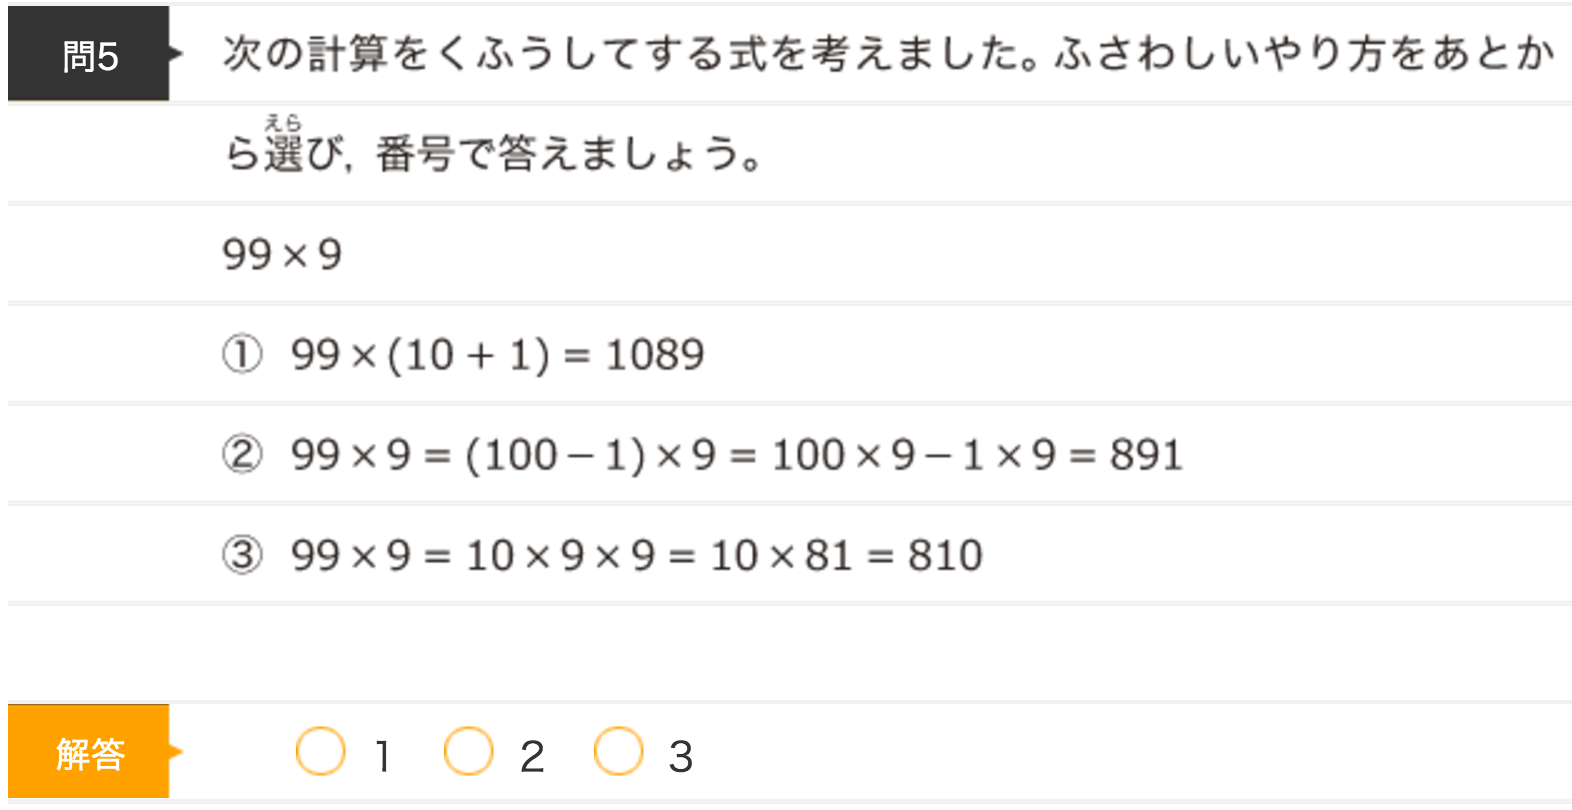
\includegraphics[width=200pt, height=150pt]{./img/qa_s4_mat.png}
	\caption{小学4年算数の問題と回答選択肢の例}
	\label{fig:qa_s4_mat}
\endminipage\hfill
\minipage{0.48\textwidth}
	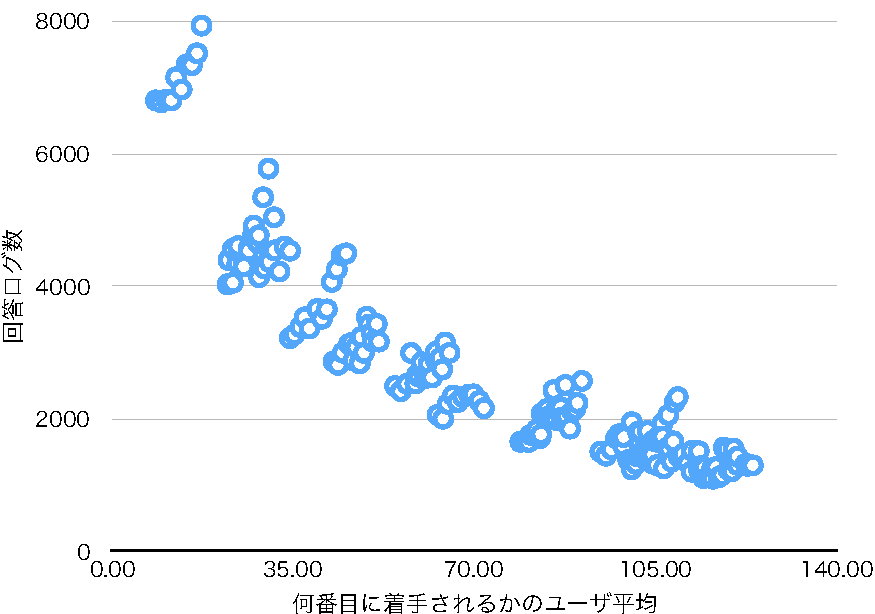
\includegraphics[width=200pt, height=150pt]{./img/stats_s4_mat.pdf}
	\caption{小学4年算数の平均着手順と回答ログ数のXYプロット}
	\label{fig:stats_s4_mat}
\endminipage\hfill
\end{center}
\end{figure}
小学4年算数では,主に,大きな数や小数など桁の認識,四則演算,数直線,折れ線グラフ,角度,分度器,垂直,並行,面積,単位,などの数理演算の基本内容が扱われる.
図\ref{fig:qa_s4_mat}に,問題と回答選択肢の例を示す.
図の問題は分配法則に関する問題であり,
その回答を選択肢のなかから選択する,という回答形式である.
次に,各問題について何番目に着手されるかの平均値と回答ログ数の関係を図\ref{fig:stats_s4_mat}に示す.
全体として,概ね1500件以上の回答ログ数があり,最初の問題の方が回答ログが大きい傾向にあるが大きく偏っているというわけではない.


\subsubsection{小学5年社会}
\begin{figure}[ht]
\begin{center}
\minipage{0.48\textwidth}
	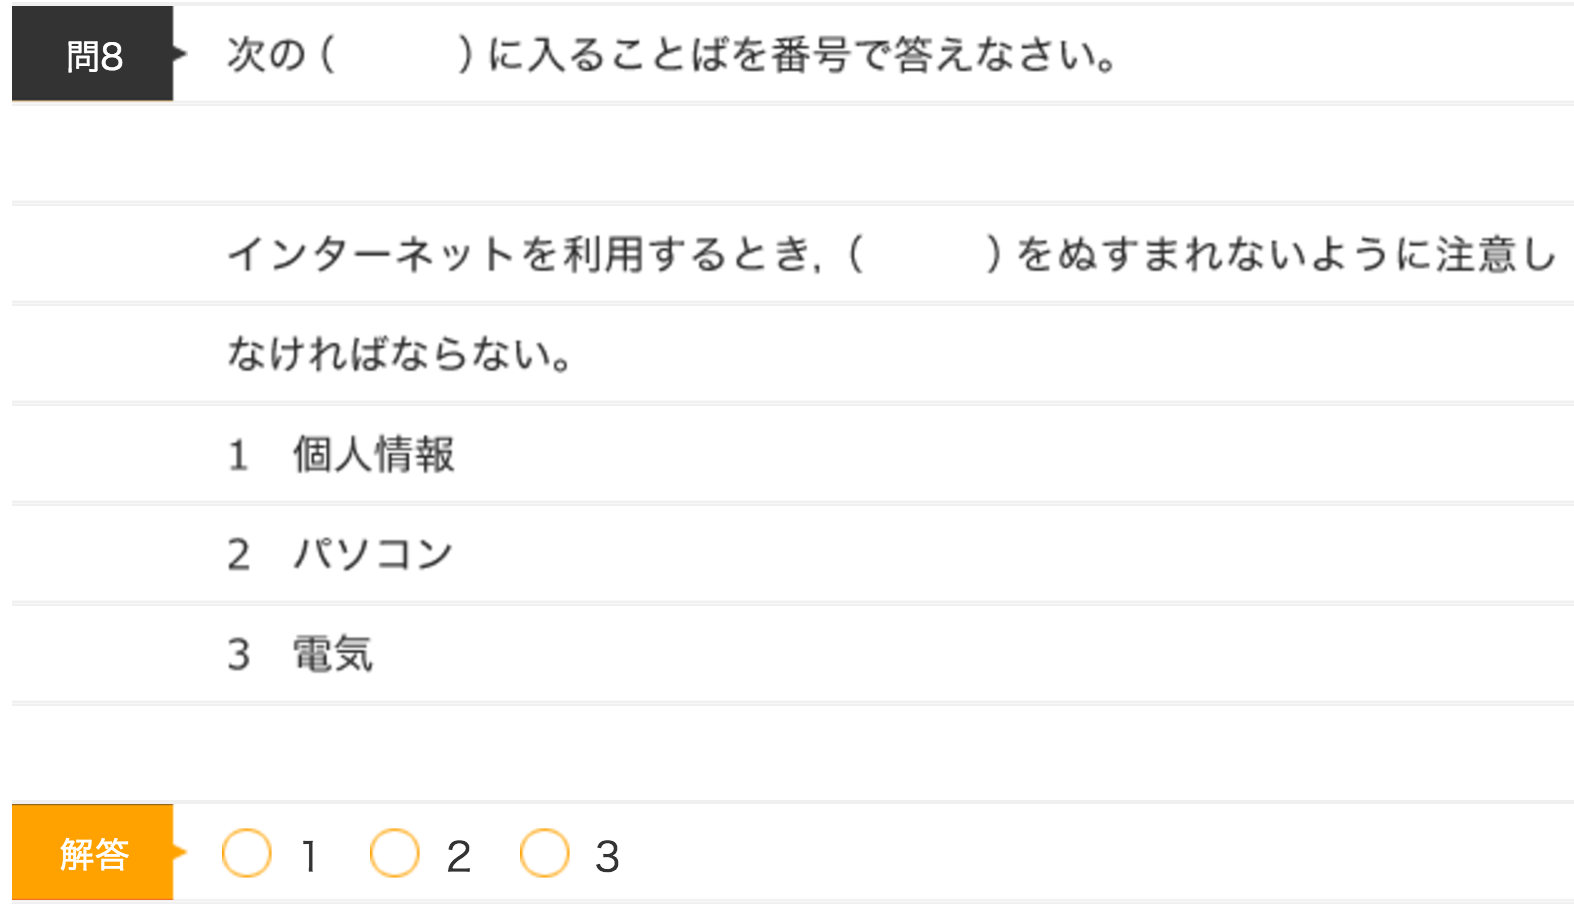
\includegraphics[width=200pt, height=150pt]{./img/qa_s5_soc.png}
	\caption{小学5年社会の問題と回答選択肢の例}
	\label{fig:qa_s5_soc}
\endminipage\hfill
\minipage{0.48\textwidth}
	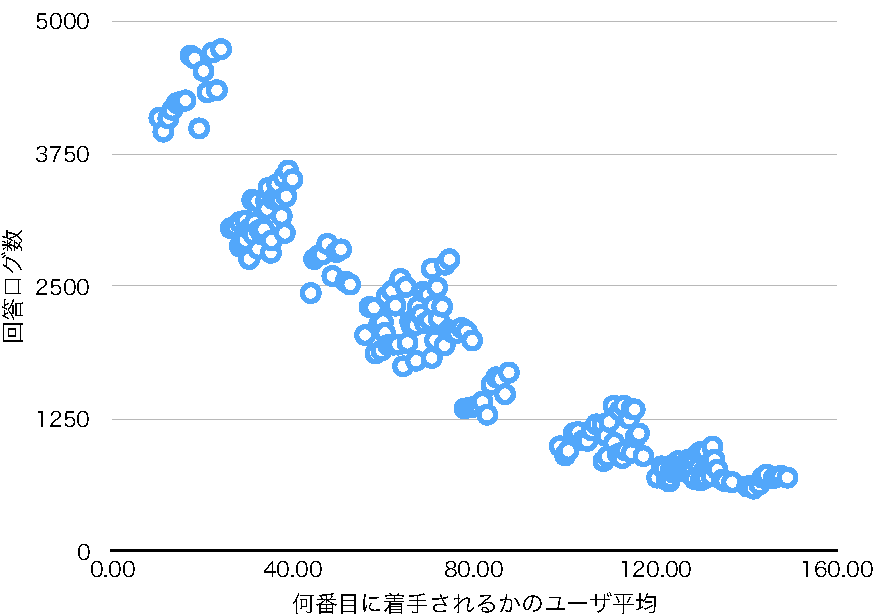
\includegraphics[width=200pt, height=150pt]{./img/stats_s5_soc.pdf}
	\caption{小学5年社会の平均着手順と回答ログ数のXYプロット}
	\label{fig:stats_s5_soc}
\endminipage\hfill
\end{center}
\end{figure}
小学5年社会では,主に,首都,地球儀,緯度経度,山地山脈,気候,平野,海流,特産物,農林水産業,輸出入,自給率,自動車などの社会基盤や社会問題に関する基本内容が扱われる.
図\ref{fig:qa_s5_soc}に,問題と回答選択肢の例を示す.
図の問題は社会問題のうち近年しばしば議論されている個人情報とインターネットに関する問題であり,
その回答を選択肢のなかから選択する,という回答形式である.
次に,各問題について何番目に着手されるかの平均値と回答ログ数の関係を図\ref{fig:stats_s5_soc}に示す.
全体として,概ね500件以上の回答ログ数があり,回答ログの分布については小学4年の社会と概ね同じである.


\subsubsection{小学5年算数}
\begin{figure}[ht]
\begin{center}
\minipage{0.48\textwidth}
	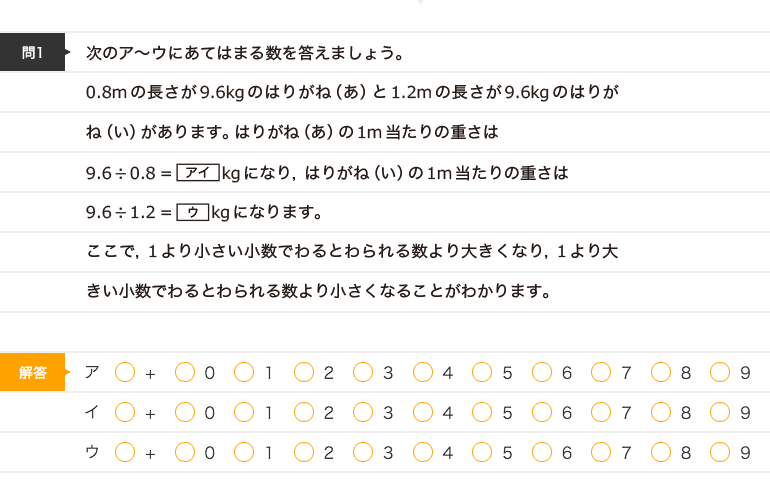
\includegraphics[width=200pt, height=150pt]{./img/qa_s5_mat2.png}
	\caption{小学5年算数の問題と回答選択肢の例}
	\label{fig:qa_s5_mat}
\endminipage\hfill
\minipage{0.48\textwidth}
	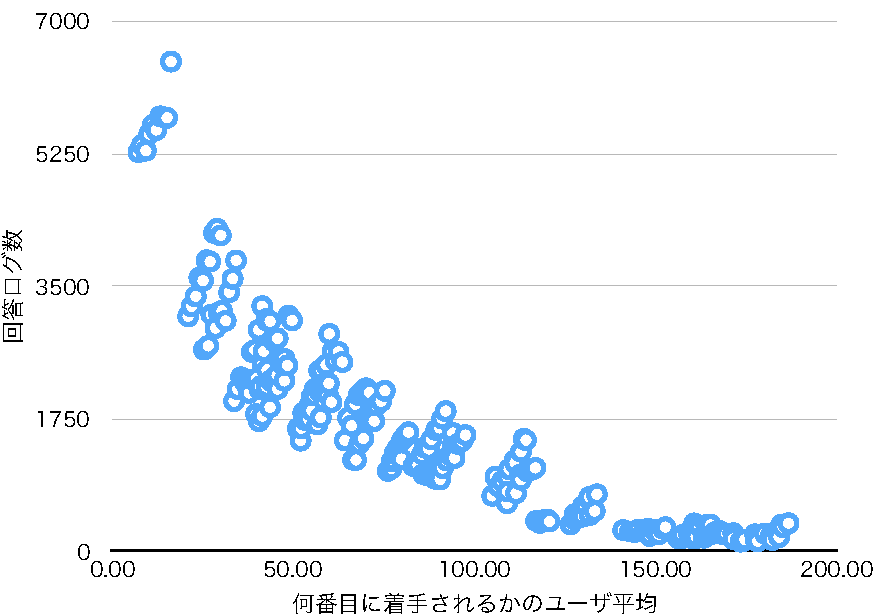
\includegraphics[width=200pt, height=150pt]{./img/stats_s5_mat.pdf}
	\caption{小学5年算数の平均着手順と回答ログ数のXYプロット}
	\label{fig:stats_s5_mat}
\endminipage\hfill
\end{center}
\end{figure}
小学5年算数では,主に,整数,約数,倍数,平行四辺形,内角,外角,展開図,円,柱,などの基本内容が扱われる.
図\ref{fig:qa_s5_mat}に,問題と回答選択肢の例を示す.
図の問題は小数の割り算に関する問題であり,
その回答を選択肢のなかから選択する,という回答形式である.
特に,回答の桁数が指定されているだけで,回答欄への自由記述に近い回答形式である.
次に,各問題について何番目に着手されるかの平均値と回答ログ数の関係を図\ref{fig:stats_s5_mat}に示す.
最後の方の問題他の問題と比べると回答ログ数がかなり小さい.


\subsubsection{小学6年社会}
\begin{figure}[ht]
\begin{center}
\minipage{0.48\textwidth}
	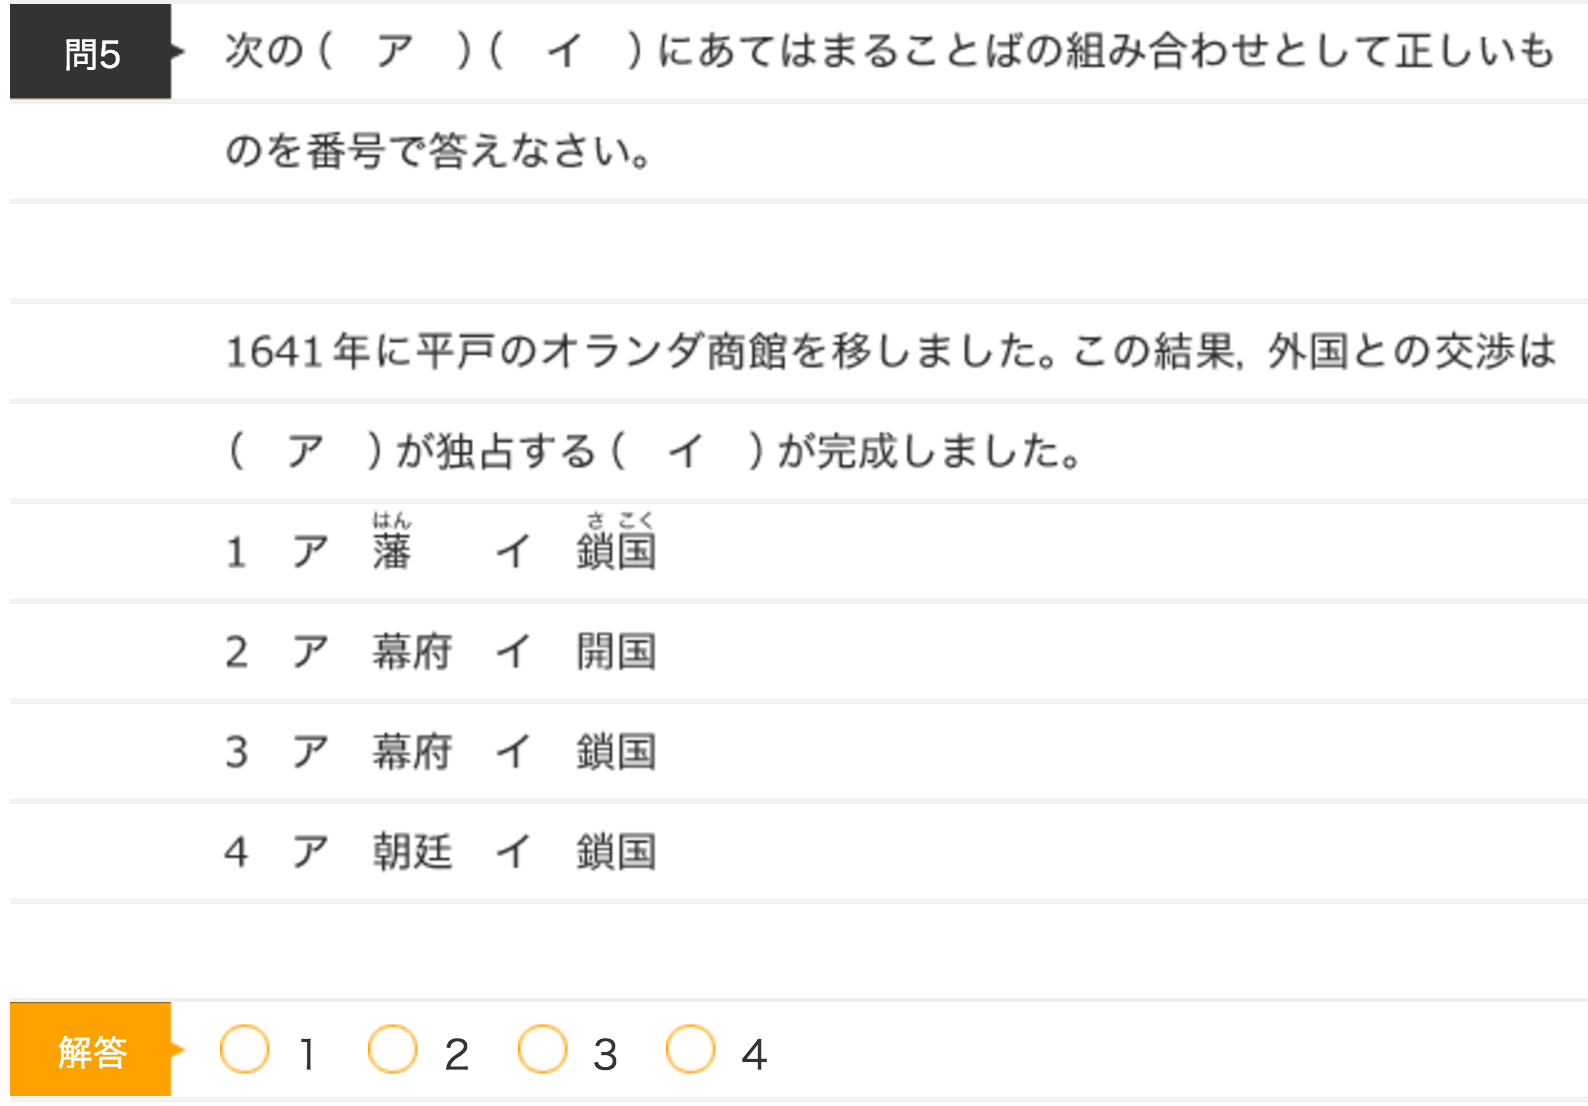
\includegraphics[width=200pt, height=150pt]{./img/qa_s6_soc.png}
	\caption{小学6年社会の問題と回答選択肢の例}
	\label{fig:qa_s6_soc}
\endminipage\hfill
\minipage{0.48\textwidth}
	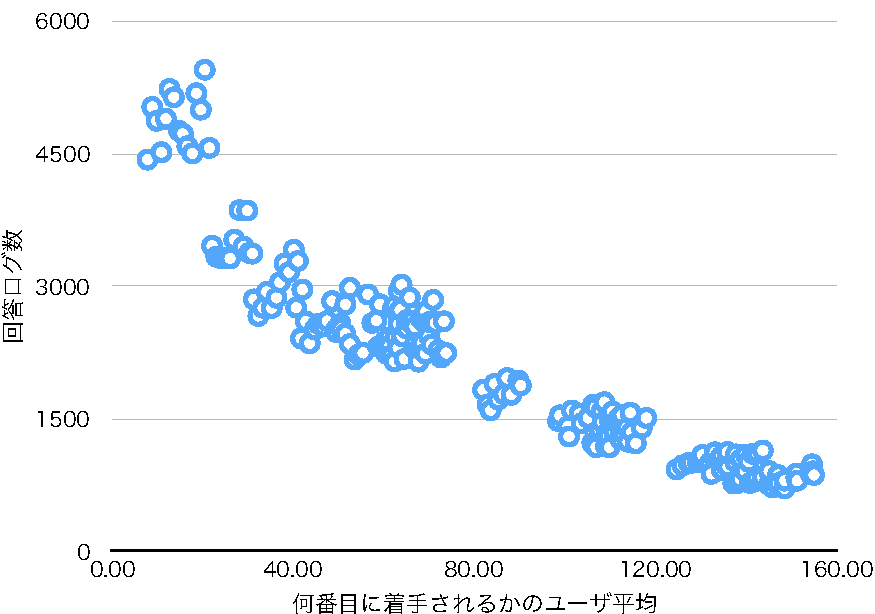
\includegraphics[width=200pt, height=150pt]{./img/stats_s6_soc.pdf}
	\caption{小学6年社会の平均着手順と回答ログ数のXYプロット}
	\label{fig:stats_s6_soc}
\endminipage\hfill
\end{center}
\end{figure}
小学6年社会では,主に,旧石器・縄文・弥生・古墳時代から昭和時代までの幅広い期間の歴史に関する内容が扱われる.
図\ref{fig:qa_s6_soc}に,問題と回答選択肢の例を示す.
図の問題は江戸時代の鎖国に関する問題であり,
その回答を選択肢のなかから選択する,という回答形式である.
次に,各問題について何番目に着手されるかの平均値と回答ログ数の関係を図\ref{fig:stats_s6_soc}に示す.
小学4年,小学5年の社会と同様に,概ね一定の割合で後半の問題の回答ログ数が減っていっていることがわかる.



\subsubsection{小学6年算数}
\begin{figure}[ht]
\begin{center}
\minipage{0.48\textwidth}
	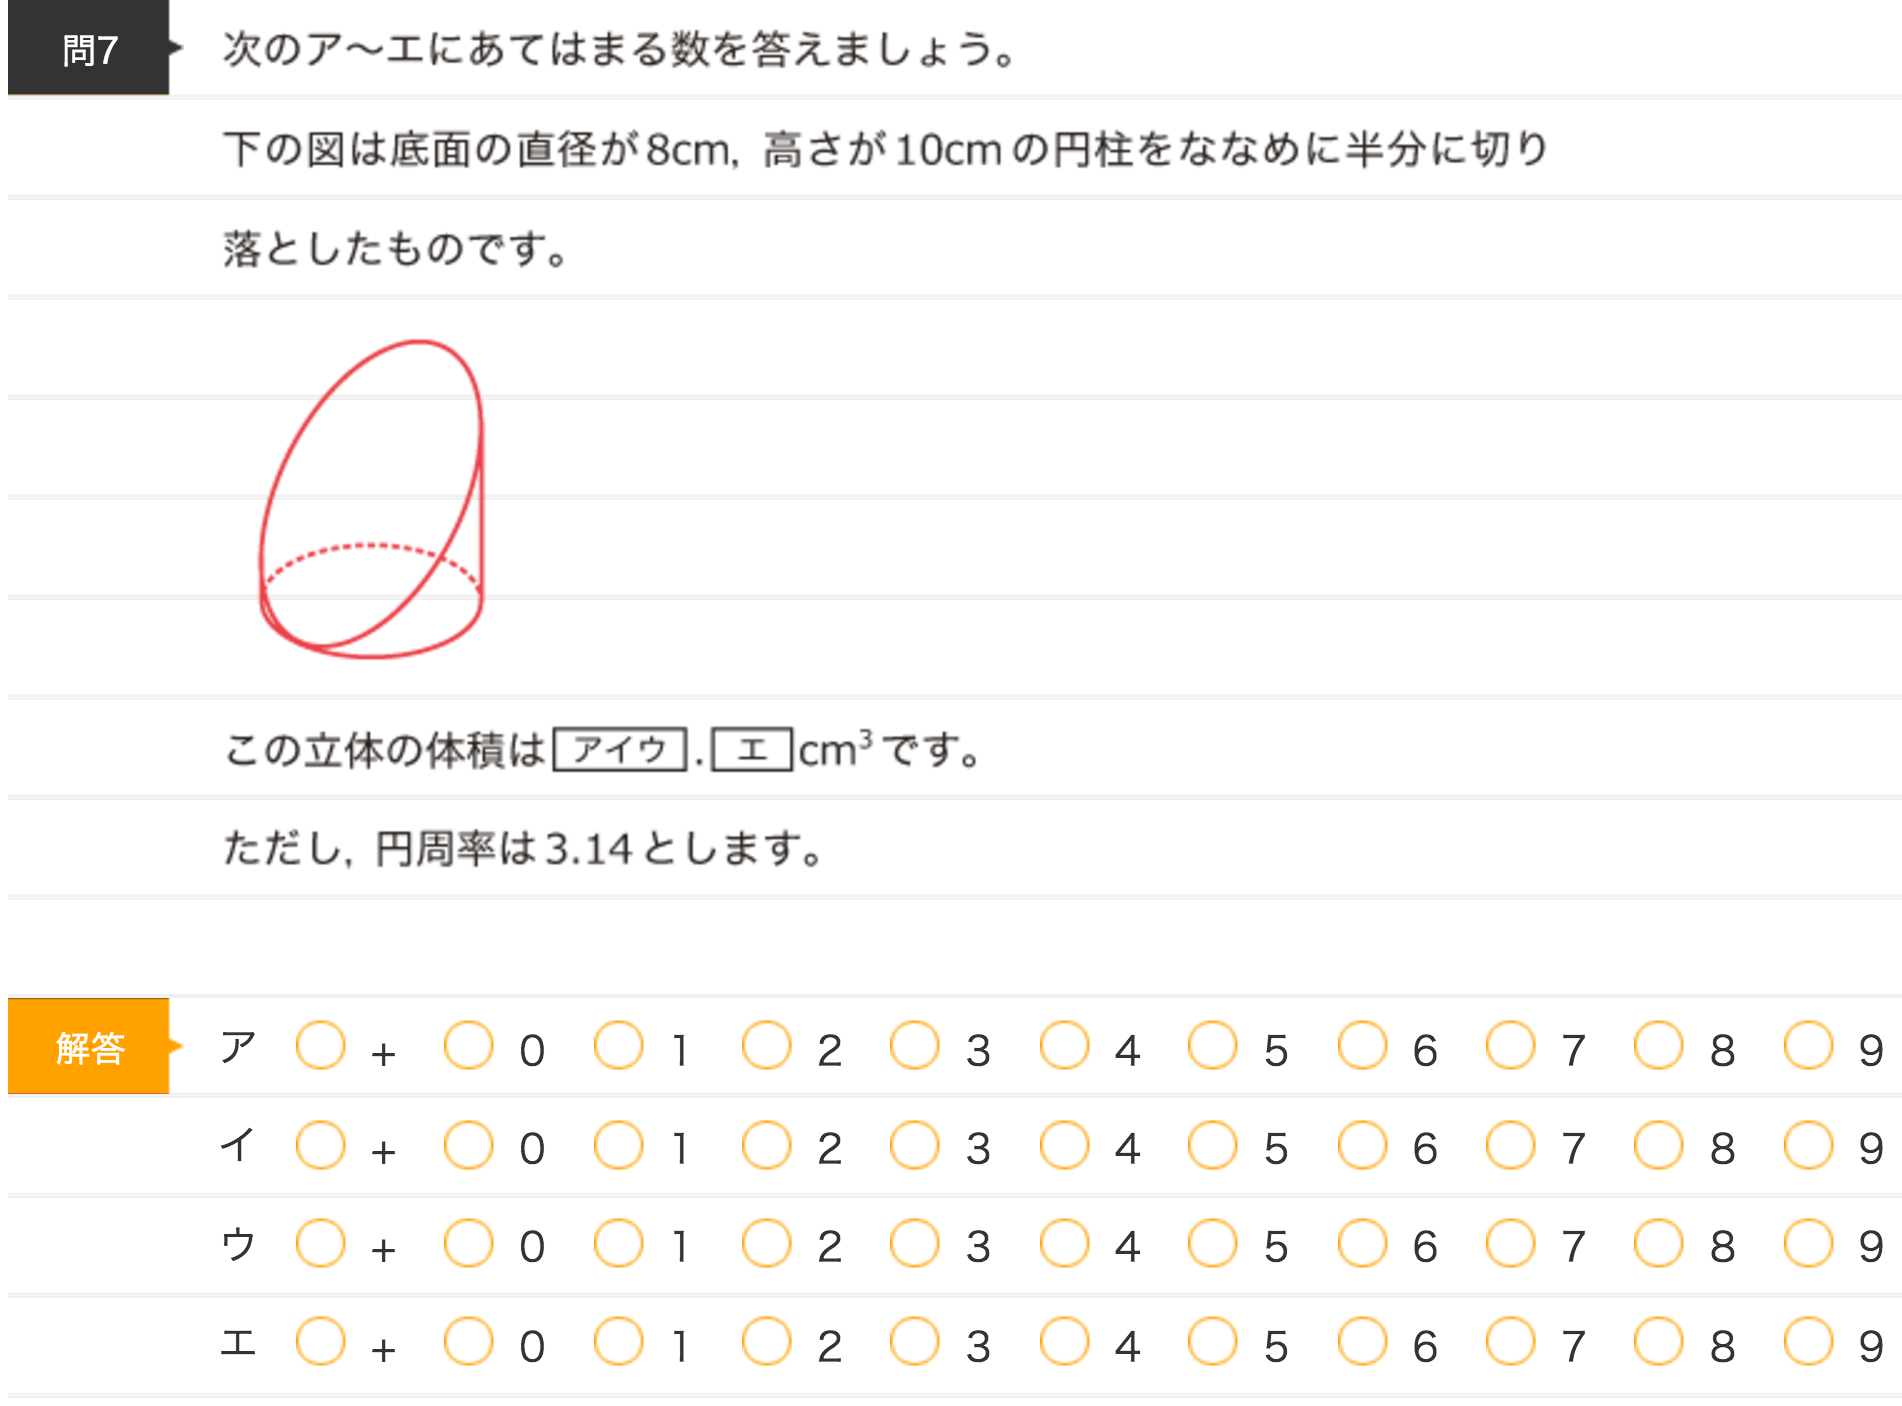
\includegraphics[width=200pt, height=150pt]{./img/qa_s6_mat.png}
	\caption{小学6年算数の問題と回答選択肢の例}
	\label{fig:qa_s6_mat}
\endminipage\hfill
\minipage{0.48\textwidth}
	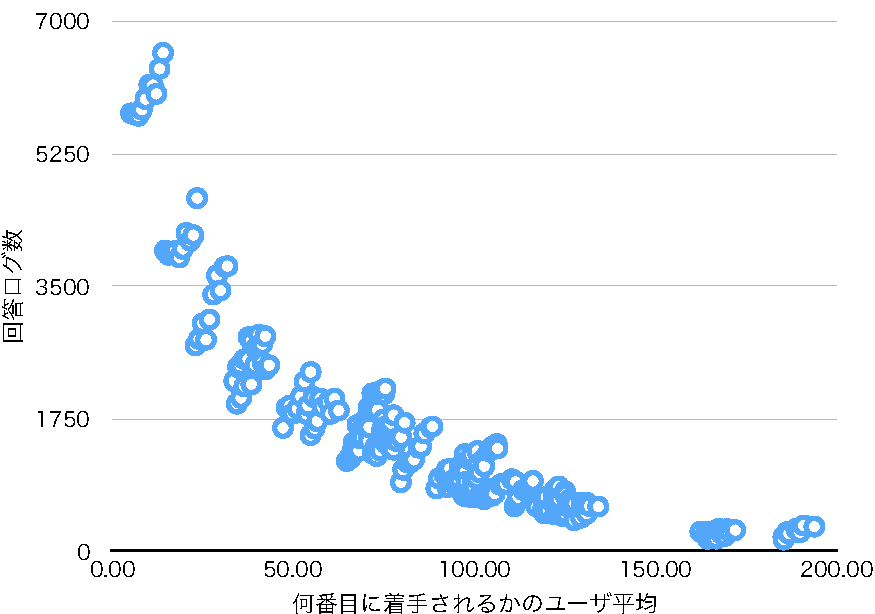
\includegraphics[width=200pt, height=150pt]{./img/stats_s6_mat.pdf}
	\caption{小学6年算数の平均着手順と回答ログ数のXYプロット}
	\label{fig:stats_s6_mat}
\endminipage\hfill
\end{center}
\end{figure}
小学6年算数では,主に,ならべ方と組み合わせ方,倍と割合,円の面積,分数のかけ算,分数のわり算,小数と分数の計算,拡大図と縮図,文字と式,比とその利用,比例と反比例,点対称,立体の体積,線対称,資料の調べ方,速さ,量と単位の基本内容が扱われる.
図\ref{fig:qa_s6_mat}に,問題と回答選択肢の例を示す.
図の問題は立体の体積のうち特に円柱の体積に関する問題であり,
その回答を選択肢のなかから選択する,という回答形式である.
特に,回答の桁数が指定されているだけで,回答欄への自由記述に近い回答形式である.
次に,各問題について何番目に着手されるかの平均値と回答ログ数の関係を図\ref{fig:stats_s6_mat}に示す.
小学4年,小学5年の算数と比べ,分布が下に凸の形になっており,
最初の方の問題への回答ログの偏りが大きいことが分かる.


\subsubsection{中学1年数学}
\begin{figure}[ht]
\begin{center}
\minipage{0.48\textwidth}
	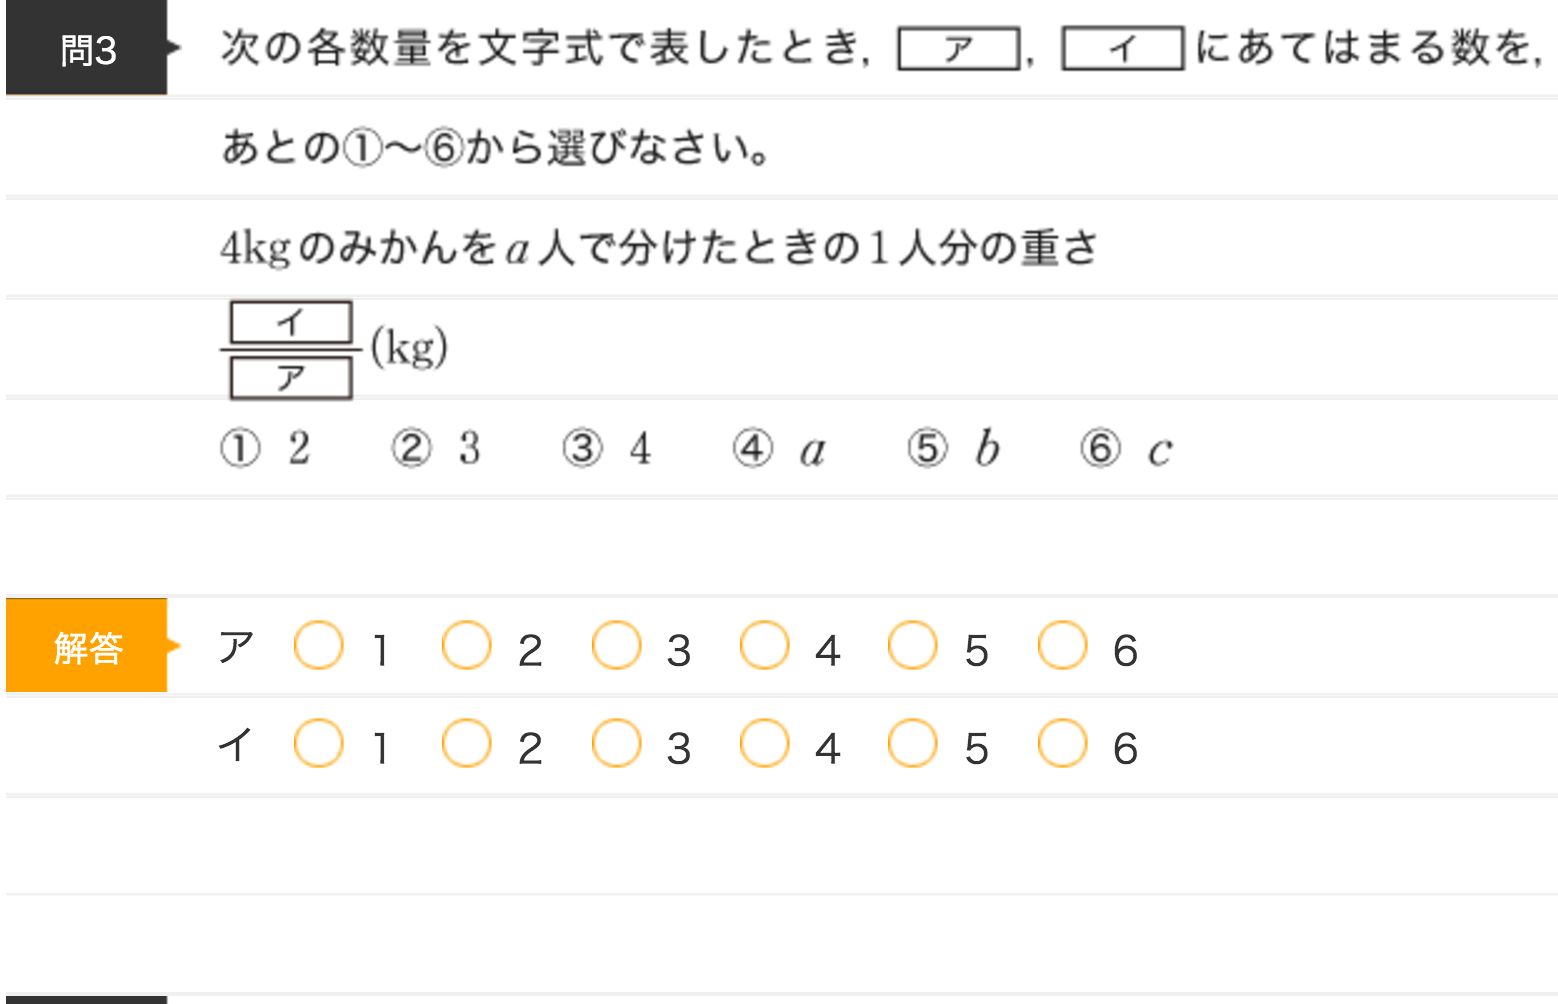
\includegraphics[width=200pt, height=150pt]{./img/qa_c1_mat.png}
	\caption{中学1年数学の問題と回答選択肢の例}
	\label{fig:qa_c1_mat}
\endminipage\hfill
\minipage{0.48\textwidth}
	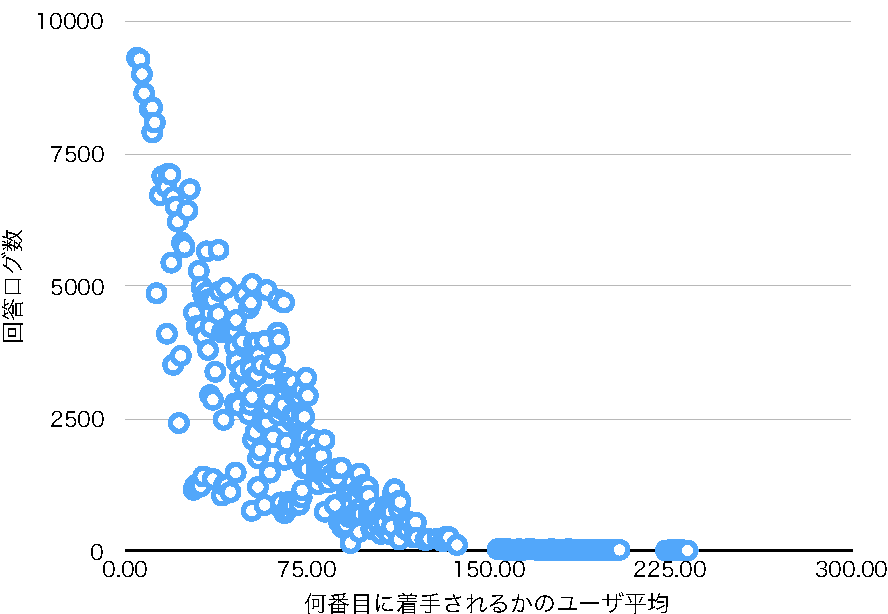
\includegraphics[width=200pt, height=150pt]{./img/stats_c1_mat.pdf}
	\caption{中学1年数学の平均着手順と回答ログ数のXYプロット}
	\label{fig:stats_c1_mat}
\endminipage\hfill
\end{center}
\end{figure}
中学1年数学では,主に,
1次式,1次方程式,2平面の関係 面の動き,代入と式の値,作図のしかた,円,反比例,図形の移動,対称移動,平面上の2直線,度数の分布,座標,数の集合と四則計算,文字式の活用,方程式,正負の数の利用,比と比例式,立体の体積,角錐と円錐
などに関する内容が扱われる.
図\ref{fig:qa_c1_mat}に,問題と回答選択肢の例を示す.
図の問題は文字式を活用した問題であり,
その回答を選択肢のなかから選択する,という回答形式である.
次に,各問題について何番目に着手されるかの平均値と回答ログ数の関係を図\ref{fig:stats_c1_mat}に示す.
回答ログは最初の方の問題に大きく偏っており,特に後半の一部は数十程度のログしかないことが分かる.


\subsubsection{中学2年数学}
\begin{figure}[ht]
\begin{center}
\minipage{0.48\textwidth}
	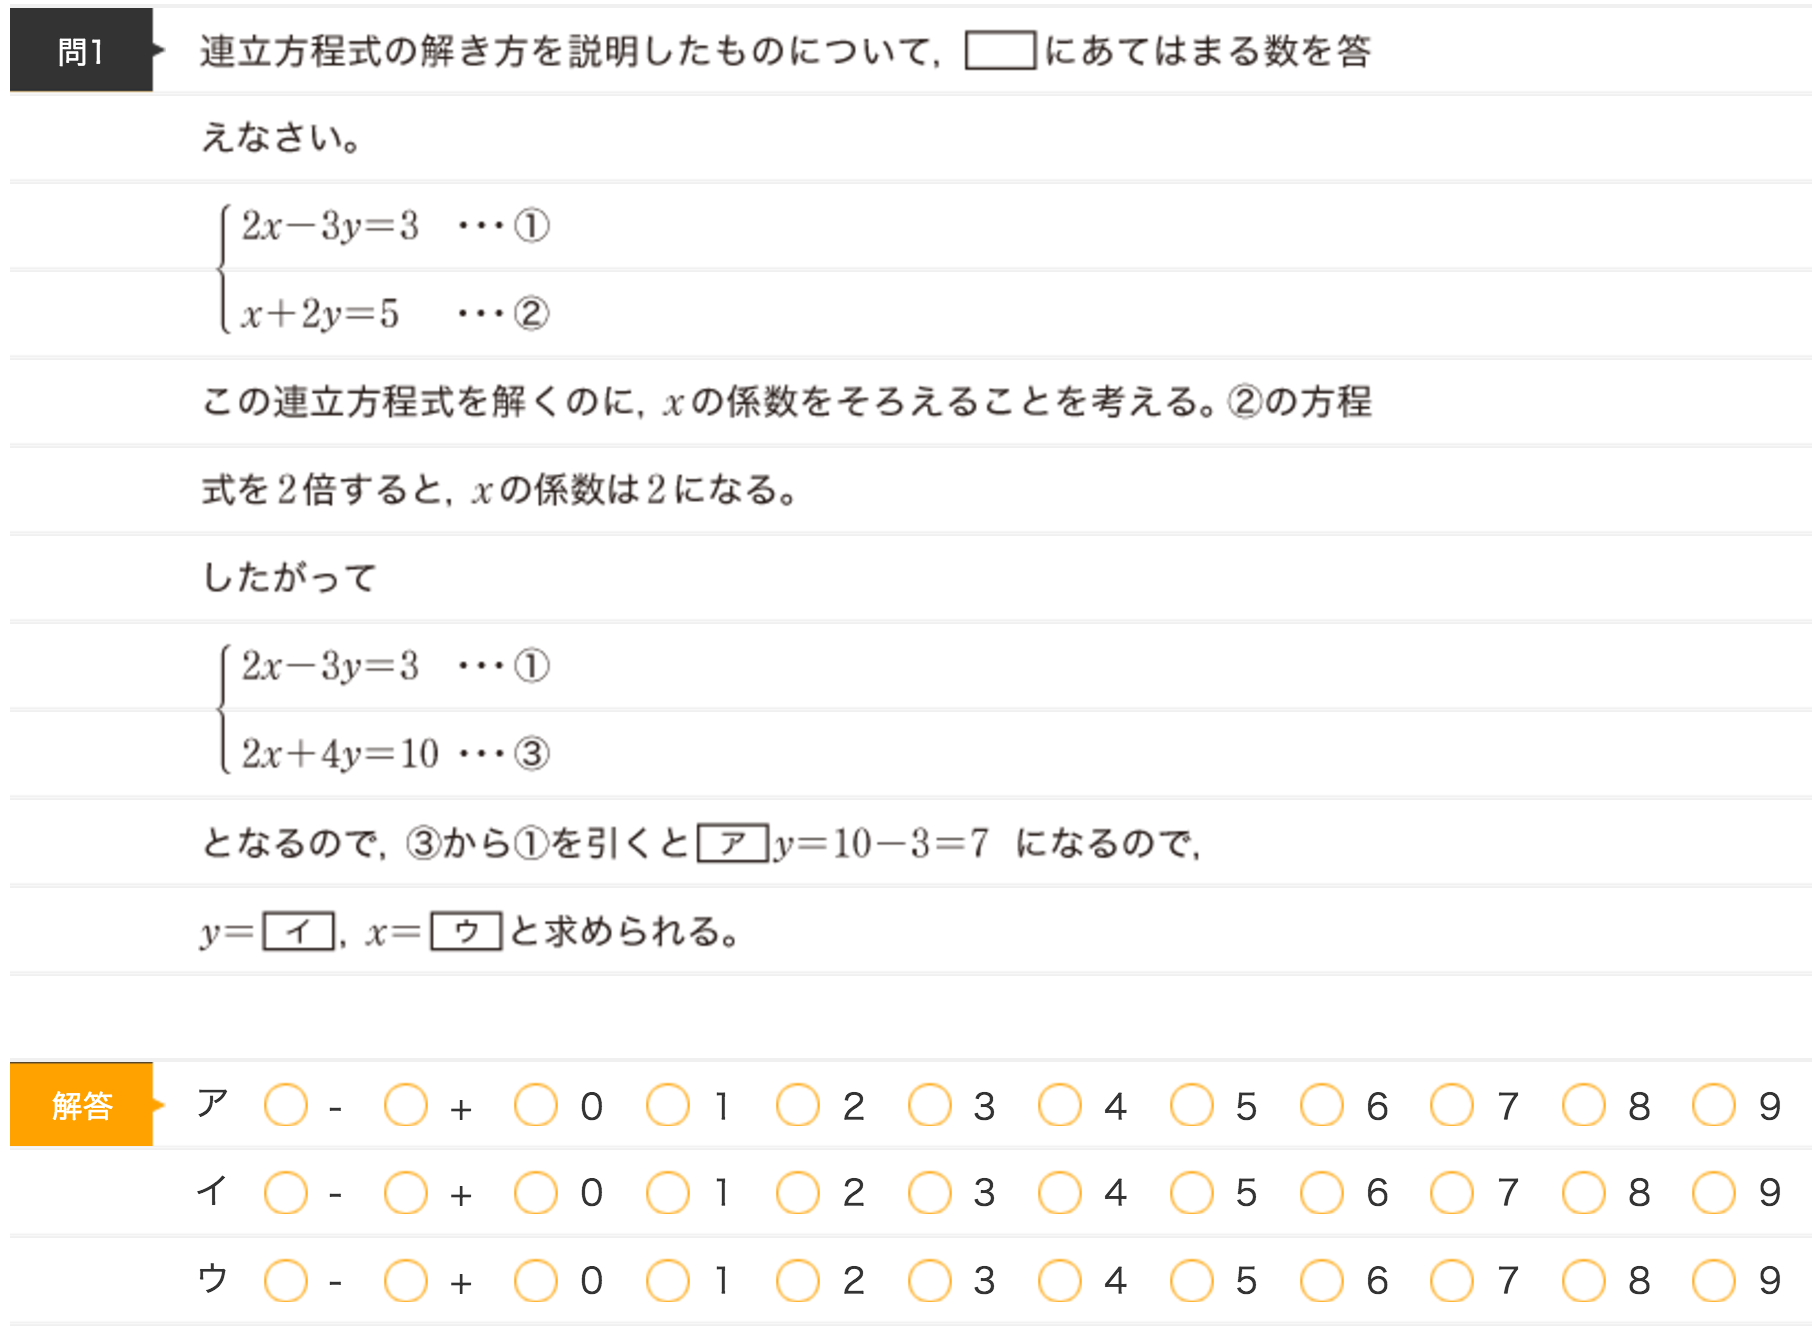
\includegraphics[width=200pt, height=150pt]{./img/qa_c2_mat.png}
	\caption{中学2年数学の問題と回答選択肢の例}
	\label{fig:qa_c2_mat}
\endminipage\hfill
\minipage{0.48\textwidth}
	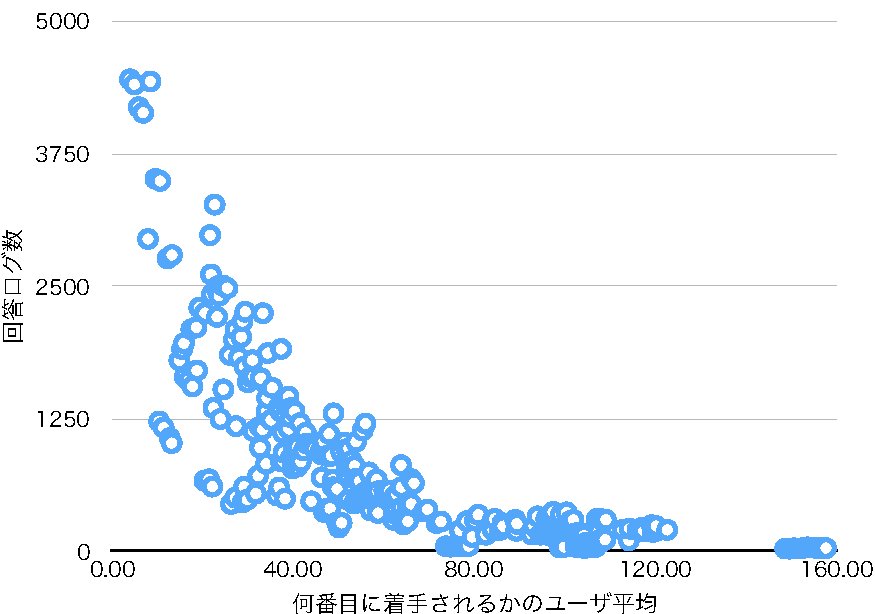
\includegraphics[width=200pt, height=150pt]{./img/stats_c2_mat.pdf}
	\caption{中学2年数学の平均着手順と回答ログ数のXYプロット}
	\label{fig:stats_c2_mat}
\endminipage\hfill
\end{center}
\end{figure}
中学2年数学では,主に,
1次方程式,1次関数,三角形の合同条件,二等辺三角形,仮定と結論,単項式と多項式,合同な三角形,平行四辺形,証明,連立方程式
などを扱う.
扱う内容は中学1年数学のデータセットのものと概ね同様であるが,難易度が高い.
図\ref{fig:qa_c2_mat}に,問題と回答選択肢の例を示す.
図の問題は数連立方程式に関する問題であり,
その回答を選択肢のなかから選択する,という回答形式である.
次に,各問題について何番目に着手されるかの平均値と回答ログ数の関係を図\ref{fig:stats_c2_mat}に示す.
グラフの外見は中学1年数学に近いが,回答ログ数のスケールが半分程度である.
また,一部の問題については,ログが数十程度と他と比べると非常に少なくなっている.


\subsubsection{中学3年数学}
\begin{figure}[ht]
\begin{center}
\minipage{0.48\textwidth}
	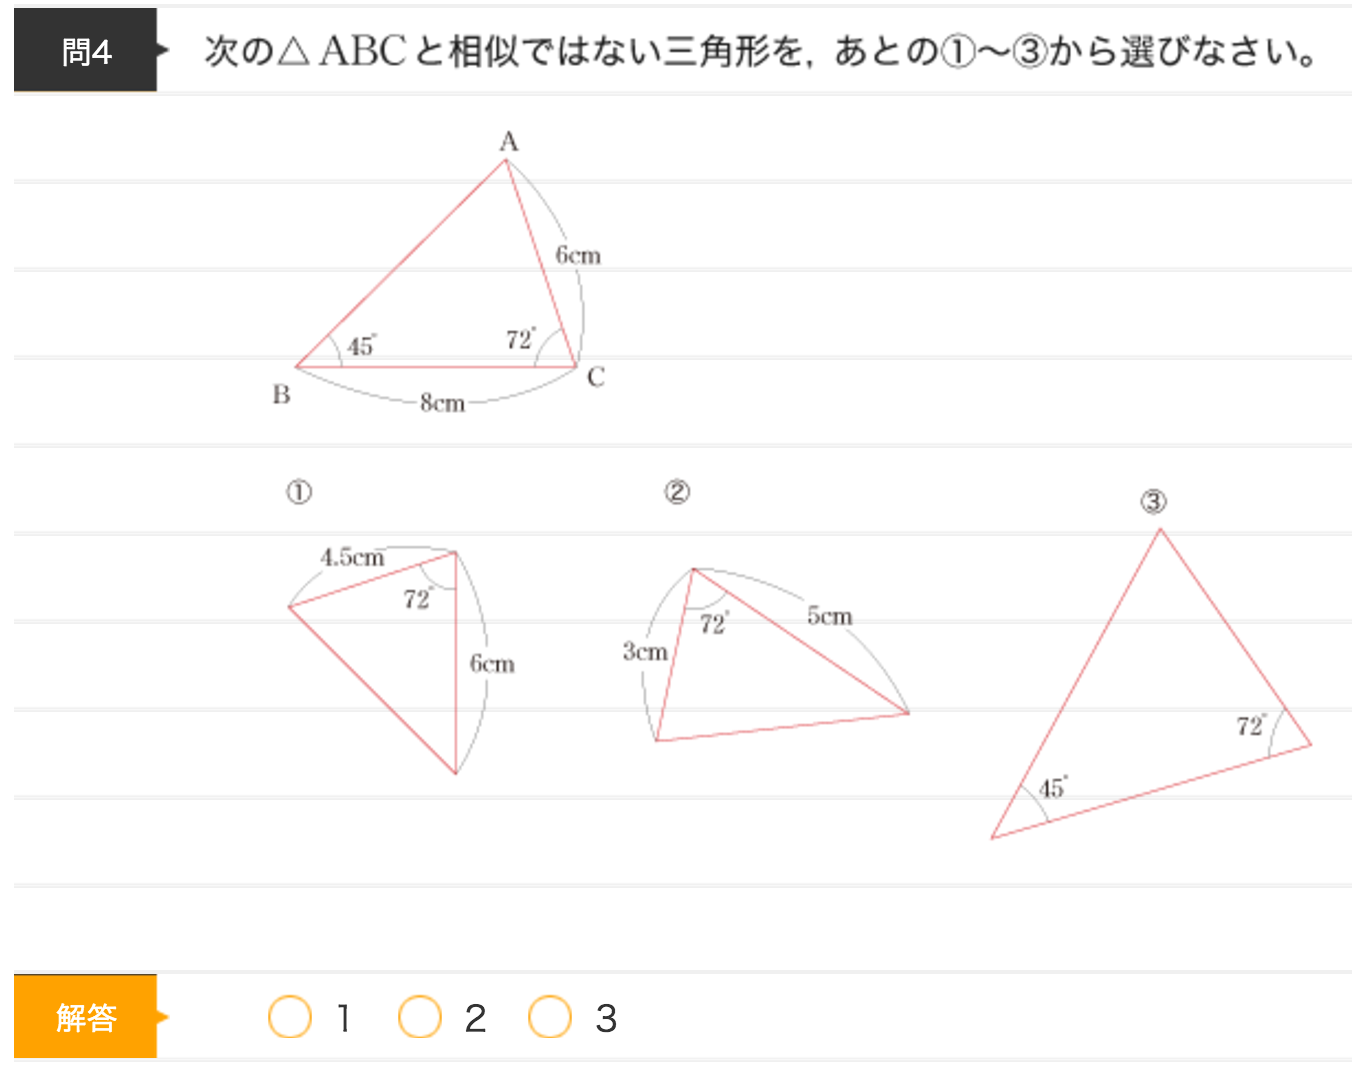
\includegraphics[width=200pt, height=150pt]{./img/qa_c3_mat.png}
	\caption{中学3年数学の問題と回答選択肢の例}
	\label{fig:qa_c3_mat}
\endminipage\hfill
\minipage{0.48\textwidth}
	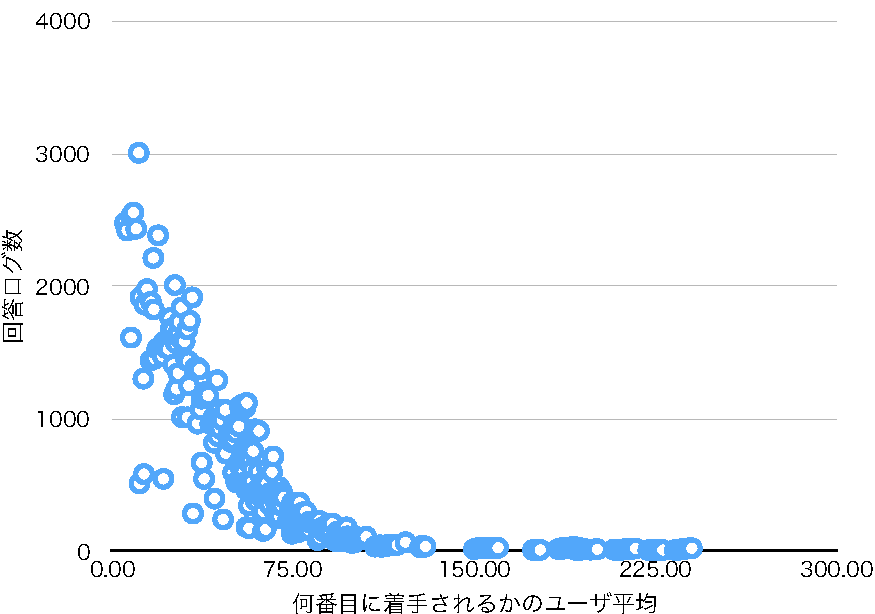
\includegraphics[width=200pt, height=150pt]{./img/stats_c3_mat.pdf}
	\caption{中学3年数学の平均着手順と回答ログ数のXYプロット}
	\label{fig:stats_c3_mat}
\endminipage\hfill
\end{center}
\end{figure}
中学3年数学では,
たすき掛け,一次関数,三平方の定理,中点連結定理,乱数表,二次方程式,二次関数,円の面積,円周角,分配法則,回転体の体積,因数分解,増加関数,変域,外接円,媒介変数,展開,平方完成,平方根,平行線,循環小数,指数,接線の定義,放物線,文字式,有理数,根号,標本調査,母集団,減少関数,無理数,相似の三角形,相似比,立方体,等差数列の和,約数,素因数分解,素数,解と係数の関係
などの内容が扱われる.
図\ref{fig:qa_c3_mat}に,問題と回答選択肢の例を示す.
図の問題は図形のうち相似の三角形に関する問題であり,
その回答を選択肢のなかから選択する,という回答形式である.
次に,各問題について何番目に着手されるかの平均値と回答ログ数の関係を図\ref{fig:stats_c3_mat}に示す.
グラフの外観は中学2年数学に類似しているが,
後半の問題の回答ログ数は非常に少ない.


\subsubsection{中学地理}
\begin{figure}[ht]
\begin{center}
\minipage{0.48\textwidth}
	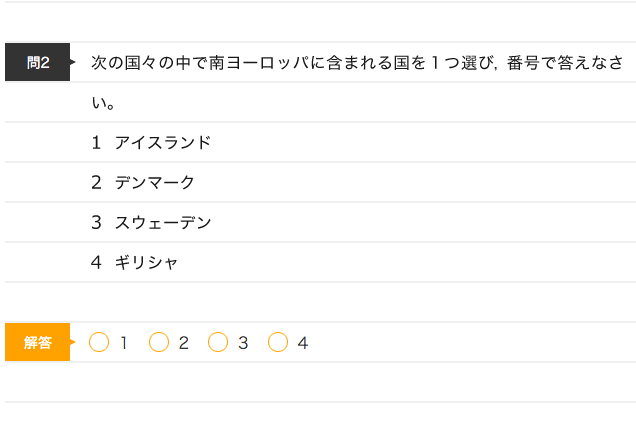
\includegraphics[width=200pt, height=150pt]{./img/qa_c_geo2.png}
	\caption{中学地理の問題と回答選択肢の例}
	\label{fig:qa_c_geo}
\endminipage\hfill
\minipage{0.48\textwidth}
	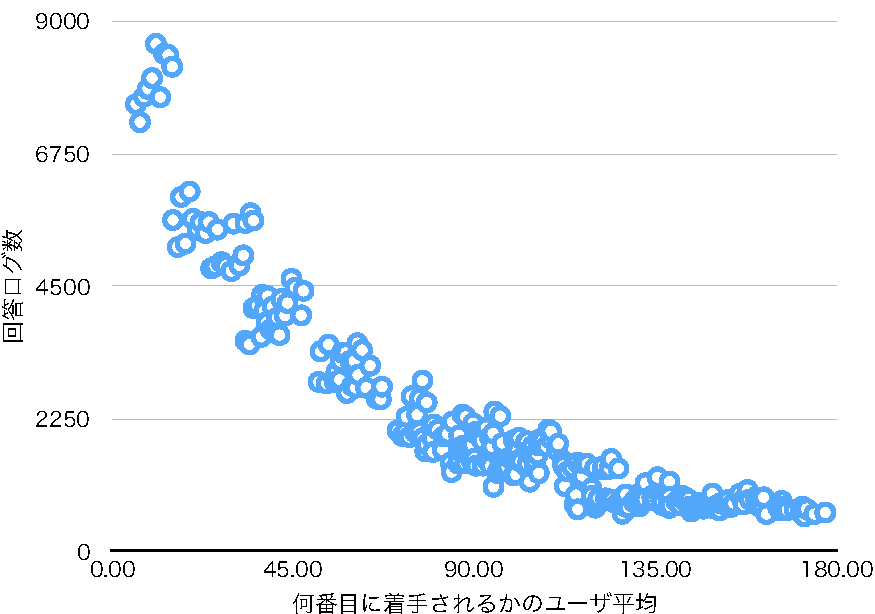
\includegraphics[width=200pt, height=150pt]{./img/stats_c_geo.pdf}
	\caption{中学地理の平均着手順と回答ログ数のXYプロット}
	\label{fig:stats_c_geo}
\endminipage\hfill
\end{center}
\end{figure}
中学地理では,主に,
アジア,アフリカ,オセアニア,ヨーロッパ,北アメリカ,南アメリカ,世界と日本の関係,世界の地域区分と特色,世界の衣食住・宗教,地域の調査,日本の地域区分,日本の工業と商業・サービス業,日本の農林水産業,東北地方,近畿地方,関東地方,中部地方,九州地方,北海道地方,中国・四国地方
などが地域や地域の性質,地域間の関係性が扱われる.
図\ref{fig:qa_c_geo}に,問題と回答選択肢の例を示す.
図の問題はヨーロッパに関する問題であり,
その回答を選択肢のなかから選択する,という回答形式である.
次に,各問題について何番目に着手されるかの平均値と回答ログ数の関係を図\ref{fig:stats_c_geo}に示す.
全体として,概ね500以上の回答ログ数があり,前半の問題から後半の問題にかけてほぼ線形に回答ログ数が減少している.


\subsubsection{中学歴史}
\begin{figure}[ht]
\begin{center}
\minipage{0.48\textwidth}
	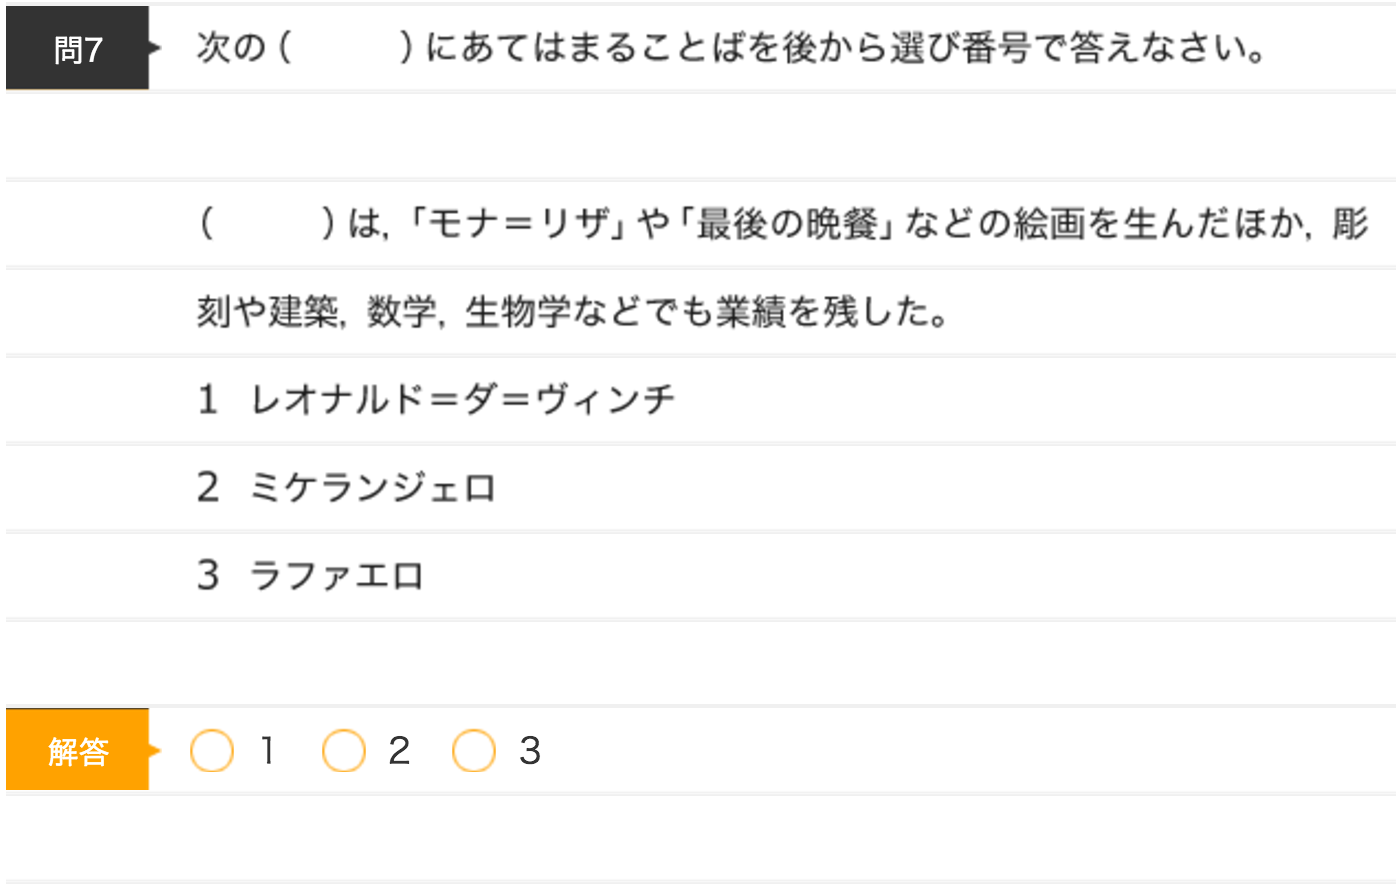
\includegraphics[width=200pt, height=150pt]{./img/qa_c_his.png}
	\caption{中学歴史の問題と回答選択肢の例}
	\label{fig:qa_c_his}
\endminipage\hfill
\minipage{0.48\textwidth}
	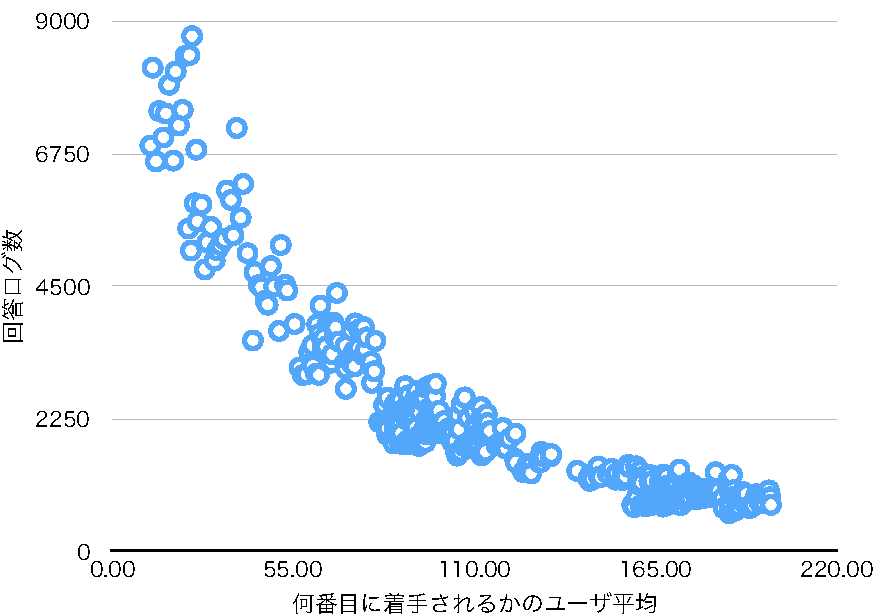
\includegraphics[width=200pt, height=150pt]{./img/stats_c_his.pdf}
	\caption{中学歴史の平均着手順と回答ログ数のXYプロット}
	\label{fig:stats_c_his}
\endminipage\hfill
\end{center}
\end{figure}
中学歴史では,主に,
ルネサンスと大航海時代,世界恐慌と国際情勢の悪化,世界文明の発生,国際協調体制,第一次世界大戦とロシア革命,欧米の市民革命と産業革命,旧石器・縄文・弥生時代,安土桃山時代,大和時代,奈良時代,平安時代,鎌倉時代,室町時代,江戸時代,明治時代,昭和時代,大正時代,平成時代
,など内容が扱われる.
図\ref{fig:qa_c_his}に,問題と回答選択肢の例を示す.
図の問題はルネサンスと大航海時代に関する問題と推察される.
その回答を選択肢のなかから選択する,という回答形式である.
次に,各問題について何番目に着手されるかの平均値と回答ログ数の関係を図\ref{fig:stats_c_his}に示す.
全体として,概ね500以上の回答ログ数があり,前半の問題から後半の問題にかけてほぼ線形に回答ログ数が減少している.
外観は中学地理と概ね合致している.


以上,個々のデータセットおよびデータが収集された講座を具体的に説明した.
具体的な内容から,
地理と歴史に関する5講座(小学4年社会,小学5年社会,小学6年社会,中学地理,中学歴史)のデータセットが
どちらかというと,宣言的知識の獲得を主目的としているデータセットであり,
算数や数学に関する6講座(小学4年算数,小学5年算数,小学6年算数,中学1年数学,中学2年数学,中学3年数学)のデータセットが
どちらかというと,手続き的知識の獲得を主目的としているデータセットであることが分かる.


また,データセットの一部の問題については他の問題と比べてログ数が数十程度と少なかったが,
それでも数十程度のログデータがあり,
そうした問題が一部に限られていることから
知識構造を抽出できると考え,このまま全ての問題をデータセットに利用する.


\vvspace
以上,データセットについて述べた.
次章では,実験について述べる.


\chapter{実験}
\label{chap:result}
\fancyhf{}
\rhead{\thepage}
\lhead{第\ref{chap:result}章 実験}
\cfoot{\thepage}


本章では,実験について述べる.

まず,実験設定について述べ,
その後,実験結果について述べる.


\section{実験設定}

本研究の実験は,大きく以下の3つのブロックに分けられる.
\begin{enumerate}
	\item 知識分類学習モデルによる知識分類の学習
	\item 学習された知識分類の知識獲得予測性能に関する検証
	\item 学習された知識分類の性質に関する比較分析
\end{enumerate}
以下では,順に,実験設定について述べる.


\subsection{知識分類学習モデルによる知識分類の学習}
\label{sec:section}
生徒の問題回答ログに対し,図\ref{fig:model}に表される知識分類学習モデルを適用し,回答正誤の予測性において最適な知識分類を抽出する.
知識タグ空間の次元数は,既存の知識タグの次元数と統一し,
「ASSISTments 2009-2010」では56,
「bridge to algebra 2006-2007」では193とした.
実際のモデルのユニットにおいては,正答ベクトルと誤答ベクトルを分けてユニットを作るため,
それぞれ2倍のユニット数で表現されている.

ハイパーパラメタについては,
%対象データが多いため学習コストの削減を狙いRNNの部分にはGRNNを用いる.
学習率の初期値を$200$,
モーメントを$0.98$,
1エポックごとに,
減衰率$0.99$として学習率を最小学習率$10$まで減衰させる.
また,勾配のノルムの最大値を$0.00001$として\cite{pascanu2013difficulty}に従い勾配に制約を設けた.
dropoutは\cite{piech2015deep}と同様に${\bf y}_t$の方向にのみかけ,
dropout率は$0.5$とした.
隠れ層のユニット数は$400$として,
各重み行列の初期化は\cite{glorot2010understanding}にしたがった.
時系列方向の誤差逆伝搬は最長で$200$まで伝搬するように制約を設けた.

これらのハイパーパラメタは実験的に高い予測性能を発揮したため設定しており,
網羅的に探索したわけではない.
通常,深層学習の手法はハイパーパラメタの数が非常に大きく,また,
計算コストが大きいため大規模な探索は行えない.
Grid SearchやRandom Search\cite{bergstra2012random}といった探索手法が提案されているが,
専門家が手で調整した方が優れていることが報告されている\cite{larochelle2007empirical, bergstra2012random}.

最適化手法は,
\ref{eq:prediction_entropy}で表される問題回答予測に関する誤差関数$L_p$と,
\ref{eq:reconstruction_error}で問題空間と知識タグ空間のReconstruction Errorを表す誤差関数を$L_r$の和である
$L$\ref{eq:total_loss}を目的関数として最小化するものである.

学習時は\cite{piech2015deep}と同様にミニバッチごとに確率的勾配降下法で目的関数を最小化する.
評価指標はAUCスコアを採用する.

2つのデータセットいずれにおいても,
訓練:検証:テスト = 8:1:1となるようにユーザを分け,
訓練ユーザのデータでモデルを構築し,
検証ユーザのデータでハイパーパラメタを調整し, 
検証ユーザのデータで精度が最も高かったモデルを
テストユーザのデータに適用し当該モデルの最終的な精度とした.

実装には
Theanoを用いた\cite{bergstra+al:2010-scipy,Bastien-Theano-2012}.
Theanoは多次元行列を含む数学的表現の定義や計算,最適化を効率的に行えるPythonのライブラリで,
深層学習の研究ではよく利用される.


\subsection{学習された知識分類の知識獲得予測性能に関する検証}

\ref{sec:section}で得られた問題空間から知識タグ空間への写像行列を離散化し,
抽出された知識分類を用いて一般的なDKTを行い,
既存の知識分類を用いた場合の精度の比較を行う.
また,本手法で抽出される知識分類と既存の知識分類の差分を明確にするため,
以下の方法で作成された知識分類を用いた場合とも比較を行う.
\begin{itemize}
\item DKTを用いず,一般的な次元圧縮手法であるPCAやAuto Encoderによって作成された知識分類
\item DKTを用いるが,Reconstruction Errorを誤差関数に入れない,一般的な埋め込みによって作成された知識分類
\end{itemize}


まず,写像行列の離散化は,いずれのデータセットにおいても,
各問題に対して最も関係性の強い知識タグのみを1とし,他を0にする方法が,
最も高い精度で知識獲得を予測できることを確認したため,
この手法を用いる.

ハイパーパラメタについては,
%対象データが多いため学習コストの削減を狙いRNNの部分にはGRNNを用いる.
学習率の初期値を$200$,
モーメントを$0.98$,
1エポックごとに,
減衰率$0.99$として学習率を最小学習率$10$まで減衰させる.
また,勾配のノルムの最大値を$0.00001$として\cite{pascanu2013difficulty}に従い勾配に制約を設けた.
dropoutは\cite{piech2015deep}と同様に${\bf y}_t$の方向にのみかけ,
dropout率は$0.5$とした.
隠れ層のユニット数は$400$として,
各重み行列の初期化は\cite{glorot2010understanding}にしたがった.
時系列方向の誤差逆伝搬は最長で$200$まで伝搬するように制約を設けた.

最適化手法は,
一般的なDKTと同じく,
\ref{eq:prediction_entropy}で表される問題回答予測に関する誤差関数$L_p$
を目的関数として最小化するものである.

学習時は\cite{piech2015deep}と同様にミニバッチごとに確率的勾配降下法で目的関数を最小化する.
評価指標はAUCスコアを採用する.

\ref{sec:section}と同様に,
2つのデータセットいずれにおいても,
訓練:検証:テスト = 8:1:1となるようにユーザを分け,
実装にはTheanoを用いた.


\subsection{学習された知識分類の性質に関する比較分析}

\ref{sec:section}で抽出された知識分類を既存の知識分類を比較分析することで,
その性質を検証する.

まず,各知識タグが回答ログに出現する頻度の分布や,紐づく問題数の分布に着目し,
知識獲得予測の精度を向上させる要因を,データの構造から分析する.
また,抽出された知識タグと既存の知識タグを,同じネットワークに配置して可視化することで,
既存の知識タグがどのように再配置され,どのようなネットワーク構造となったのかを分析する.




以上,実験設定について述べた.



\section{実験結果}
実験結果について述べる.
まず,各手法によって作成された知識分類についての知識獲得予測における予測性能を比較し,
いずれのデータセットいずれにおいても,
提案手法によって学習された知識分類から作成された知識タグを利用することで,
最も良い精度で予測が可能になっていることを定量的に確認する.

さらに,学習された知識分類を,既存の知識分類と比較することにより,
その性質を定性的に分析する.



\subsection{各知識分類の知識獲得予測における予測性能}

%\begin{table}[!htb]
\begin{table}[t]
\caption{各知識分類の知識獲得予測における予測性能}
\label{tab:result1}
\begin{center}
\centerline{
{
\begin{tabular}{c|rrrrrr}\hline
\multirow{3}{*}{データセット}	&	\multicolumn{6}{c}{AUC}\\\cline{2-7}
 							&	\multirow{2}{*}{既存タグ(marginal)} 	& \multicolumn{2}{c}{事前圧縮タグ} 	&	& \multicolumn{2}{c}{深層学習タグ}\\\cline{3-4}\cline{6-7}
							&										& PCA 	& 	AutoEncoder	& 				& Embedding 	& AutoEncoder \\\hline 			 
%ASSISTments 2009-2010 50 	&				0.81 (0.66) 			& 0.00 	& 	0.00 	& 					& 0.00 			& {\bf 0.86}\\
ASSISTments 2009-2010 	 	&				0.76 (0.61)				& 0.?? 	& 	0.?? 	& 					& 0.?? 			& {\bf 0.78}\\
bridge to algebra 2006-2007 &				0.80 (0.70) 			& 0.?? 	& 	0.?? 	& 					& 0.?? 			& {\bf 0.85}\\
\hline
\end{tabular}
}
}
\end{center}
\end{table}



ベースラインとなる既存の知識タグ(既存タグ)と,
知識分類学習モデルから作成された知識タグ(深層学習タグ),
さらに,差分検証のための,深層学習モデルを用いずに通常の次元削減によって作成された知識タグ(事前圧縮タグ)
を,各データセットから作成し,Deep Knowledge Tracingに適用した結果を表\ref{tab:result1}に示す.
marginalは各問題についてそれぞれ正解の周辺確率を予測結果とするものである.
\cite{piech2015deep}にも記載されていたため,本稿でも同様にベースラインとして記載した.
また,
値が大きい箇所は太字で記載した.


いずれのデータセットにおいても,
提案手法である「深層学習タグ(AutoEncoder)」が,最も高いAUCを記録した.


\subsection{学習された知識分類の可視化と概観}
最も良い予測性能を発揮した「深層学習タグ(AutoEncoder)」を可視化し,その概要を明らかにする.
(ネットワークや対応関係と絡めて執筆予定)


\subsection{学習された知識分類の比較分析}
抽出された知識タグを既存の知識タグと比較することにより,
抽出された知識タグの性質を定性的に確認する.

まず,各知識タグが回答ログに出現する頻度の分布や,紐づく問題数の分布に着目し,
知識獲得予測の精度を向上させる要因を,データの構造から分析した.(図xx)
図より,既存タグは各指標について分散が大きい一方で,
抽出タグは各指標について分散が小さく,特定の値の周辺に集中している.
この分布の違いと予測精度の関係性についても,次章で考察する.

次に,
既存のDKTの手法に基づき作成された既存タグの知識間ネットワークに対し,
既存タグと抽出タグの共起行列からTD-IDF値を求めて作成した行列を元にノードとエッジを追加したネットワーク図を図xxに示す.
図より,
表より,複数の抽出タグにおいて特徴的と判断されている既存タグが存在する一方,
特定の抽出タグ内にまとめられ,他のタグでは特徴的でないと判断されている既存タグも存在する.
この特徴付けにより,どのような性質のタグが抽出されているかについては,次章で考察する.



\vvspace
以上,実験について述べた.
次章では,考察について述べる.




\chapter{考察}
\label{chap:discussion}
\fancyhf{}
\rhead{\thepage}
\lhead{第\ref{chap:discussion}章 考察}
\cfoot{\thepage}

本章では,実験結果を踏まえた考察を述べる.

まず,
知識分類の予測性能の比較実験の結果から,
本研究で用いた知識分類学習モデルの有効性について考察する.
次に,同モデルにより抽出された知識分類と既存の知識分類を比較し,
性質の違いとそれが知識獲得予測に与える影響について考察する.
また,本研究や関連研究が対象としたデータの範囲から,
手法の汎用性や成果の実用性について考察し,
本研究の実用的・学術的価値について述べる.

最後に,
今後の展望として,
より良質な知識分類を得るためのモデルの改善案について述べた後,
本研究で用いた手法の学習科学での適用の可能性について述べ,
最後に,学習科学以外の分野への応用可能性について述べる.

%粒度
%汎用性
\section{本手法の有効性と知識分類の解釈}
まず,本手法で用いた知識分類学習モデルの有効性と,それによって得られた知識分類についての解釈を行う.


\subsection{知識分類学習モデルの有効性}
知識獲得予測の性能の比較実験の結果から,
本研究で用いた知識分類学習モデルの有効性について考察する.


まず,既存の知識分類を利用した場合と,各手法によって抽出した知識分類を利用した場合の,知識獲得予測の精度に関して考察する.
実験結果より,知識獲得予測の文脈を考慮せず,事前学習のAutoEncoderのみから作成した知識分類(事前学習タグ)を用いた場合は,
既存の知識分類(既存タグ)を用いた場合よりも精度が悪かった一方で,
知識分類学習モデルにより,知識獲得予測を最適化する過程で抽出した知識分類(提案手法タグ)は,
既存タグよりも精度の良いものがあった.
この状況を直接的に解釈すれば,知識分類は,
データ構造のみに着目する教師なし学習では,知識獲得予測に有効な表現として学習できないが,
知識獲得予測という目的に応じた環境情報を制約に加えて学習することで,その環境と矛盾しないような知識分類が抽出できたと考えられる.
また,より教育学的な文脈を踏まえて解釈を試みれば,
問題と知識分類はそれ自体で自明な関係ではなく,
問題を回答する生徒の回答正誤や知識獲得の推移という状態の観測を通して定義されることで,適切な表現になるものだと見なすことも可能である.

知識獲得予測の文脈を考慮した提案手法タグにおいては,
データ数が比較的少ない「ASSISTments 2009-2010」では,
単純な低次元空間への埋め込み($L_p$)に加えて問題空間とタグ空間の再構成誤差を導入($L_p + L_r$)したことにより,精度が向上した.
これは,
データ量の不足に対する正則化項の導入という,ニューラルネットワークの文脈における,データの量的側面と,
問題の回答正誤と知識タグの理解状態は相互に変換できるはずだという,教育学の文脈における,データの質的側面との,
双方の性質を活かす最適化の要素として,再構成誤差が効果を発揮したと考えられる.

さらに,再構成誤差に加えてスパース正則化項を加えた場合($L_p + L_r + L_s$)が,いずれのデータセットにおいても最も高い精度を示した.
これは,最終的に写像行列を離散化する際に,情報ロスが少なくなるような形式で情報量を保てる,疎な行列として写像行列が学習されたためだと考えられる.

%また,知識獲得予測の文脈を考慮した提案手法タグにおいても,
%単純な低次元空間への埋め込み($L_p$)では精度が向上しないものの,
%再構成誤差とスパース正則化項を加えた($L_p + L_r + L_s$)ことにより,精度が向上した.
%これは,再構成誤差については,
%データ量の不足に対する正則化項の導入という,ニューラルネットワークの文脈における,データの量的側面と,
%問題の回答正誤と知識タグの理解状態は相互に変換できるはずだという,教育学の文脈における,データの質的側面との,
%双方の性質を活かす最適化の要素として,再構成誤差が効果を発揮したと考えられる.
%また,スパース生息加工については,最終的に写像行列を離散化する際に,情報ロスが少なくなるような形式で情報量を保てる,スパースな行列として写像行列が学習されたためだと考えられる.

結果的に,知識獲得予測の文脈において最適化させ,再構成誤差とスパース正則化項を導入した「提案手法タグ($L_p + L_r + L_s$)」が最も高い精度を発揮し,
提案手法の各要因が知識分類の最適化に効果を発揮したことが検証されたといえる.
以下,この「提案手法タグ($L_p + L_r + L_s$)」を「抽出タグ」とする.


\subsection{各知識分類の性質と知識獲得予測に与える影響}
次に,既存タグと抽出タグのそれぞれの性質の違いに着目し,それがどのように知識獲得予測に影響をあたえるのかを考察する.

まず,図\ref{fig:AppearHist}に表される,既存タグと抽出タグの回答ログにおける出現回数の分布から,
既存タグは偏りが大きい一方で,抽出タグは偏りが小さく,特定の値の周辺に集中していることがわかった.
既存タグは,学問の伝統的な背景や人間にとっての可読性に基づいて作成されており,
その知識を問う問題が回答される回数は作成時の評価軸に含まれていない.
そのため,基礎的・入門的な問題に関しては多くの生徒に回答される一方,
専門的であったり難易度の高い問題に関しては,回答される回数が必然的に少なくなるため,
タグ間で出現回数に差が出る.
しかし,Deep Knowledge Tracing(DKT)のモデルに入力される際には,どの知識タグも均等に1つのユニットで表現されるため,
実際の知識獲得過程において各知識タグが持つ情報量の偏りを十分に表現できない可能性が高い.
一方,抽出タグは,DKTを拡張した知識分類学習モデルで学習されているため,
各ユニットが均等に情報量を保つことが可能になり,
DKTに適用した場合にも特定のタグに関する情報量が失われることを防いでいると考えられる.

この性質は,タグ関係ネットワーク図にも現れている.
図\ref{fig:NetworkConcentrate},\ref{fig:NetworkLittle}に表されるように,
元々出現回数が少ない専門的な既存タグは,少数の抽出タグ(緑のノード)のみで表現されているが,
逆に元々出現回数の多い基礎的な既存タグは,複数の抽出タグにまたがって表現されるなど,
より効率的に情報を保持できるタグ構造となっていることがわかる.

さらに,こうした情報量の均等な分配構造は,内容と全く無関係に生成されるものではないこともわかる.
図\ref{fig:NetworkSimilar}に表されるように,
「ASSISTments 2009-2010」では「Probability of Two Distinct Events(二つの異なる事象の確率)」「Percent Of(百分率)」「Venn Diagram(ベン図)」という,確率や場合の数の内容に当たる既存タグが,
「Bridge to Algebra 2006-2007」では「Identify GCF(最大公約数を求める)」「Identify number as common factor(公約数を求める)」「Identify number as common multiple(公倍数を求める)」という,公約数や公倍数の内容に当たる既存タグが,
それぞれ一つの抽出タグによって表現されているように,
類似した内容の範囲内で情報量の分配を行っている抽出タグが見受けられる.
こうしたタグは,情報量を適切に保ちつつ関連知識一般をカバーするようなタグである可能性が高く,
人間が知識を獲得していく過程を考察する上で示唆に富んでおり,さらなる研究の価値がある.



\section{本手法の汎用性と実用性}
次に,本研究や関連研究が対象としたデータの範囲から手法の汎用性について述べ,
また,本手法の教育現場への適用について考察し,本手法の実用性について考察する.
%
%\subsection{学習された知識分類の汎用性}
%知識分類学習モデルによって学習された知識分類の汎用性について考察する.
%
%一般的な機械学習では,モデルの汎化性能を高めるためにデータを訓練データと検証データに分けるが,
%本研究の知識分類学習モデルでは,全ユーザの問題回答ログを全て訓練データとして,モデルを学習させた.
%このようなデータの利用の仕方は,訓練データの分布において最適な結果が得られる一方,
%未知のデータに対する汎用性が担保されないため,一般的ではない.
%しかし,本研究においては,
%知識獲得予測を最適化する知識分類を抽出することを目的とし,
%その手段として,過去の生徒の知識獲得の過程から,帰納的に最適な知識分類を作成するという形を取っており,
%これはすなわち,将来の生徒の知識獲得過程は,過去の生徒の知識獲得の過程と同じ分布に従うという前提に立っている.
%また,オンライン教育サービスにおいては,日々新たな学習回答ログが蓄積されるため,
%その都度知識分類を更新し,より質の高い分類を作成できるという環境が整っている.
%以上より,本研究の問題設定においては,これまでの知識獲得過程を全てまとめて訓練データとしても,
%学習された知識分類の汎用性は損なわれず,
%また,未知のデータが出現した際にも即座にそれを反映し,より適切な知識分類を作成できると判断したため,
%知識分類の学習の時点では全データを訓練データとした.
%なお,学習された知識分類の性能を検証するDKTの部分においては,既存タグとの精度比較の公平性を期すために,データを訓練・検証・テストに分割している.
%
%一方で,
%現在観測されているデータと将来観測されているデータの分布が大きく異なる可能性がある場合や,
%未知のデータが出現した場合に即座にそれを分類に反映させることが困難な場合には,このようなデータの分割方法は相応しくない.
%そのような場合には,全データを訓練・検証・テストに分割することで,
%学習された分類の汎化性能を保証する必要があり,
%環境や問題設定に応じたデータの扱いや,環境に左右されないモデルの設計が今後の課題といえる.


\subsection{本手法の他データへの適用可能性}
本手法の汎用性を,他の科目やオンライン教育サービスへの適用可能性の観点から考察する.
まず,本研究の手法は,
データセット作成という事前の処理と,以下の3つの分析から構成されていた.
\begin{enumerate}
	\item 知識分類の学習と抽出
	\item 知識分類の予測性能の検証
	\item 知識分類の性質の比較
\end{enumerate}

データセット作成については,オンライン教育サービスから収集される問題回答ログデータは,サービスや科目によらず大規模であると考えられる.
また,実験の「2.知識分類の予測性能の検証」,および「3.知識分類の性質の比較」は,
知識分類学習モデルによって,適切な知識分類を学習できるかに依存する.
よって,本手法の他科目や他サービスへの適用可能性は,「1.知識分類の学習と抽出」に依存すると考えられる.
知識分類学習モデルはDKTを拡張したモデル構造において学習されるため,
DKT自体の他科目や他サービスへの適用可能性によって,本手法の適用可能性も検証されると考えられる.


そこで,DKTの他科目や他サービスにおける適用可能性を考察する.

\cite{piech2015deep}では,本研究同様,数学に関するデータセットにおいてのみ,DKTの有効性が検証されていたが,
\cite{nasuno2016深層学習}はリクルートが提供するオンライン教育サービス「勉強サプリ」\footnote{現,「スタディサプリ」.\url{https://benkyosapuri.jp/}}のデータを使って,
算数や数学に関するデータセットと地理や歴史に関するデータセットにDKTを適用した場合,
Bayesian Knowledge Tracingからの精度向上という点では大きな差はないことを確認しており,
DKTの適用可能性は科目に依らない可能性が高い.

また,
\cite{piech2015deep}を始めとする既存研究では,モデルへの入力次元には問題に割り当てられたタグが利用されており,
DKTの有効性はタグを用いた場合のみ,検証されていた.
本研究の実験では,
問題回答ログのみから知識分類を学習できるため,
既存の知識分類が存在せず,タグ付けができないような科目やサービスのデータに対しても,
生徒の知識獲得を予測することが可能であることを示している.


一方で,これまで検証されているのは,
特定の科目に関する問題回答ログであり,
総合的な知識レベルを問うような,複数の科目が含まれている問題回答ログへの適用可能性は示されていない.
また,利用できるデータセットは,生徒が該当のオンライン教育サービスで学習する過程で,
段階的に知識を獲得していく前提のデータのみであり,
オンライン教育サービス外での学習や,生徒ごとの能力差,事前知識などの情報に関しては,
DKTが扱うことは難しい可能性がある.


以上のような考察を踏まえると,
本手法は,DKTが分析可能な他サービスや他科目のデータに加え,
DKTによる分析が困難な,事前の知識分類が存在しないデータに対しても適用できるという側面がある一方,
複数科目のデータや生徒に関する事前情報など,
現実に即した複雑な情報が多く含まれたデータに対しては,適用可能性が限定的である可能性もあり,検証が必要である.
% このような例として具体的にどのようなデータが考えられるか?


\subsection{本手法の教育現場への適用と実用的・学術的価値}
ここまでの考察を踏まえ,本手法を実際の教育現場に適用し,活用する方法を述べ,
教材推薦システムの精度向上と,構造化されていない学問の構造化という観点から,
本研究の実用的・学術的価値を考察する.


そもそも,
オンライン教育サービスにおける知識獲得の予測は,
問題を正答するのに必要な知識を生徒が既に獲得しているかを推定することで,
不足している知識を補ったり,既に獲得している知識を除外したりと,
適切な順序で教材推薦を行うことが実用上の主な目的であった.
本研究の実験結果から,本手法によって抽出された知識分類を利用することにより,知識獲得の予測精度が向上することが確認されており,
知識獲得の予測精度が向上するということは,
各生徒の知識状態をより的確に把握して,教材推薦の精度を向上させることを意味する.
よって,
現在オンライン教育サービス上で提供されている問題に対して,
既存の可読性重視の知識分類に加え,本手法によって抽出された知識分類を紐付けておくことで,
教材推薦の精度が向上することにより,生徒個人個人への教材の最適化が進み,生徒の学習効率をより高めることができる.
この知識分類の粒度は,本研究では既存の知識分類との比較のために固定としていたが,自由に設定することが可能なため,サービスごとに適切な粒度を設定することが可能である.


また,本手法は,現存の教材推薦システムの精度を向上させるだけでなく,
これまで構造化されていなかった学問を構造化することも可能である.
近年のオンライン教育サービスの普及に伴い,
これまでの伝統的な学問体系の範疇を超えた新たな学問が続々登場しており,
まだその体系が十分に構造化されておらず,また誰が何を持って構造化するのかという点が曖昧な学問が多数存在する.
本手法は,人間による事前の知識分類を必要とせずに,知識獲得の文脈において最適な知識分類を作成することが可能であるため,
このような未成熟な学問体系を定量的な根拠に基づいて構造化する事が可能である.
知識を構造化し,かつそれを最適なものにするということは,
生徒の学習効率を向上させ,また
指導者にとっても,既存の教材やカリキュラムを再検証したり,より効果的な教材を考える事が可能にするため,
その学問の発展の上で大きな意義を持つ.

以上のような理由から,
定量的な根拠に基づいて最適に構造化されていなかったり,そもそも構造化されていないような未成熟な学問体系に対して,
本手法を用いて知識獲得の予測性を最適化するように構造化し,知識分類を作成することは,学術的にも,実用的にも価値が高い.


\section{今後の展望}
本研究の今後の展望について大きく3つの方針を述べる.
まず,本手法をさらに改善し,より良質な知識分類を学習できるようなモデル構造の可能性について述べ,
次に,学習科学における対象データの拡大について述べ,
最後に,学習科学以外の分野への本手法の応用について述べる.


\subsection{知識分類学習モデルの改善}
本研究では,知識獲得の予測性を最適化する知識分類を抽出するにあたり,
まず,知識分類学習モデルに問題回答ログを入力して問題空間から知識タグ空間への写像行列を学習し,
その行列を離散化することで,タグを抽出していたが,
連続値の行列を人間の手によって離散化することにより,情報量のロスが避けられなかった.
また,連続表現の知識分類の予測性能と,離散表現の知識分類の予測性能が線形関係にあるとは限らないため,
最適な連続表現を得てそれを離散化したとしても,最適な離散表現が得られるとは断言できない.

よって,得られた知識分類が最適な離散表現であることを確実に示すには,初めから離散表現のタグを深層学習によって最適化し,学習できることがより望ましい.
これは,問題の集合の背後にタグの離散的な確率分布が存在することを仮定し,知識獲得予測を最適化させるような分布を学習することによって,最適な離散表現のタグを学習するタスクとして設定できる.
データが生成された確率分布を深層学習によって学習するには,一般的な機械学習の識別モデルとは異なる,生成モデルの研究領域における,Variational Autoencoder(VAE)の技術が利用できる\cite{kingma2014semi}.
%VAEでは,学習目的の確率分布からサンプリングを行って分布を学習していく.
%本来サンプリングという行為は微分不可能な関数によって表されるため,誤差逆伝播による学習が不可能だが,
%サンプリング対象の確率分布を生成する別の確率分布を定義するReparameterization Trickと呼ばれる手法により,
%微分可能な関数として学習することが可能になった.
%この確率分布は,分布をパラメータ化し,深層学習の勾配法によってそのパラメータを最適化することによって学習されるものであるため,
%分布が微分可能な関数として記述される必要がある.
%そのため,微分不可能な関数で表現される離散分布は勾配法によって学習できないため,生成モデルによって推定することは不可能とされていたが,
%近年考案されたreparameterization Trick\cite{}と呼ばれる手法を用いることにより,
従来のVAEで学習できるのは連続的な確率分布のみとされていたが,
近年の研究により離散分布についても学習することが可能になったことが報告されている\cite{maddison2016concrete, jang2016categorical}.
この手法を知識分類学習モデルに組み込めば,
問題と知識タグの関係性として潜在的な離散分布を仮定し,この分布を学習することにより,
勾配法による最適化によって直接最適な離散表現を得ることが可能だと考えられるため,
今後の研究課題である.




\subsection{学習科学における対象データの拡大}
次に,学習科学における対象データの拡大について述べる.
対象データの拡大とは,科目や難易度の多様化,予測期間の長期化,そして複数科目の統合である.


まず,科目や難易度の多様化について述べる.
本研究では.数学の問題回答ログに対して深層学習を適用し,知識獲得の予測性を最適化する知識分類を得た.
これまでのDKTの研究成果から,数学以外の教科に対しても適用できる可能性は高いが,実際にどのような知識分類が抽出されるかは分析していない.
また,今回扱ったデータセットは,小学校から高校程度の数学に関する問題回答ログであり,より高度で専門的な大学レベルの学問に適用する場合についても,どのような知識分類が抽出されるかは分析していない.
知識獲得予測の最適化に関する知見は,学校側からの指導や生徒自身の学習設計に活用されており,多様な難易度や科目において知識獲得を最適化する知識構造を明らかにすることは,重要であると考えられる.


次に,予測期間の長期化について述べる.
本研究で用いたデータセットの対象期間は,1〜2年程度であった.
しかし,知識分類学習モデルによって学習される知識分類は,それまでの生徒の知識獲得の過程に依存しており,
できるだけ長い期間の知識獲得を分析するほうが,より適切な知識分類を抽出できる可能性は高い.


最後に,複数科目の統合について述べる.
本研究や既存研究では,特定の科目について独立に知識獲得を予測し,知識構造を分析している.
しかし,実際の生徒の学習の成長過程は,科目間で完全に独立であるとはいえず,
例えば,歴史と地理や,数学と物理などの科目間では,知識獲得の過程が密接に関係している可能性がある.
一人の生徒の,科目を横断した知識獲得過程に関する研究は,これまで報告されていないが,
複数科目を統合したデータに対して本手法を適用し,
科目を横断した知識分類や包括的な学習設計に関する知見を得ることは,学術的な意義が大きいといえる.


\subsection{学習科学以外の分野への応用}
最後に,本手法の学習科学以外の分野への応用について述べる.

本論文が研究対象としたのは,Knowledge Tracingという,
学習科学の研究分野における知識獲得予測の手法だが,
より手法を一般化することで,学習科学以外の分野にも応用できる可能性を秘めている.

本手法は,
生徒の時系列問題回答ログから,
回答を重ねるごとに遷移していく知識状態をモデリングし,
知識獲得の過程を適切に表現する知識分類を抽出するというものだが,
これをより一般化して捉えると,
人間の,何らかのコンテンツ集合に対する時系列行動ログから,
行動を重ねるごとに遷移していく人間の何らかの状態をモデリングし,
行動の遷移を適切に説明する分類表現を抽出し,構造化しているといえる.
知識獲得予測においては,
このコンテンツ集合に対する行動が生徒の問題回答であり,
問題回答により遷移する生徒の知識状態をモデリングしているが,
これと同様のことは,学習科学に限らず行える可能性がある.
例えば,消費者が商品を購買する時系列ログを分析することで,
消費者の嗜好が遷移する過程をモデリングし,
従来の商品分類と異なる,消費者の嗜好の遷移を反映した分類を抽出することが可能になり,
消費者の購買予測の精度が向上したり,これまでとは異なる系統の商品推薦が行える可能性がある.

知識獲得予測では,問題回答の正誤と知識の間の特殊な関係性をモデル設計に反映しているように,
手法を適用する領域によって調整は必要であるが,
手法の根本的な特性として,コンテンツに対する時系列行動を反映した分類を抽出して構造化できる可能性は高く,
様々な領域で,学術的にも,実用的にも,価値の高い知見や成果を得られると考えられる.


\chapter{結論}
\label{chap:conlusion}
\fancyhf{}
\rhead{\thepage}
\lhead{第\ref{chap:conlusion}章 結論}
\cfoot{\thepage}


本論文では,
既存の知識獲得予測における問題として,
人間が作成した知識分類を利用していることを指摘し,
深層学習を適用することによって,
知識獲得の予測性において最適化された知識分類を抽出できることを検証した

また,抽出された知識分類を定量的・定性的に分析することにより,
知識の内容的な関係性と,分類ごとの回答に関する情報量を最適に分配することが,知識獲得の予測性の向上に寄与することがわかった.
\vvspace

本研究の成果を実際の教育現場で活用例として,教材推薦システムへの適用を論じ,
既存の手法では困難だった,他の科目やオンライン教育サービスへ適用できる可能性がある一方,
複数科目を統合した知識獲得や,大学水準の知識獲得に関しては,検証実験を行う必要が有ることを述べた.
\vvspace


さらに,本研究の拡張として,
より良質な知識分類を学習するために活用できる最新の深層学習技術や,
適用対象データの拡張について述べ,
また,より一般性を高めた議論として,
学習科学以外の領域においても本手法が適用できる可能性に触れ,
人間行動に関する多様な知見を発見できる可能性を論じた.
\vvspace

本研究は.
教育と情報技術の融合の進展やオンライン教育サービスの普及,教育分野における大規模分析の活発化や深層学習の躍進など,
ここ数年の多様な領域の進展によって初めて可能になったものである.
本研究が,新たな教育システムの構築,そして人間の学習や知識の解明につながると信じている.



\newpage
\addcontentsline{toc}{chapter}{参考文献}
\label{chap:reference}
\fancyhf{}
\rhead{\thepage}
\lhead{参考文献}
\cfoot{\thepage}

%\bibliographystyle{junsrt}
\bibliographystyle{apalike}
\bibliography{biblio}



\appendix
\chapter*{付録}
\label{chap:appendix}
\fancyhf{}
\rhead{\thepage}
\lhead{付録:各講座のネットワーク図}
\cfoot{\thepage}

\begin{figure}[!htb]
\begin{center}
	\hspace*{-10pt}\makebox[1.2\textwidth][c]{
		\minipage{0.52\textwidth}
			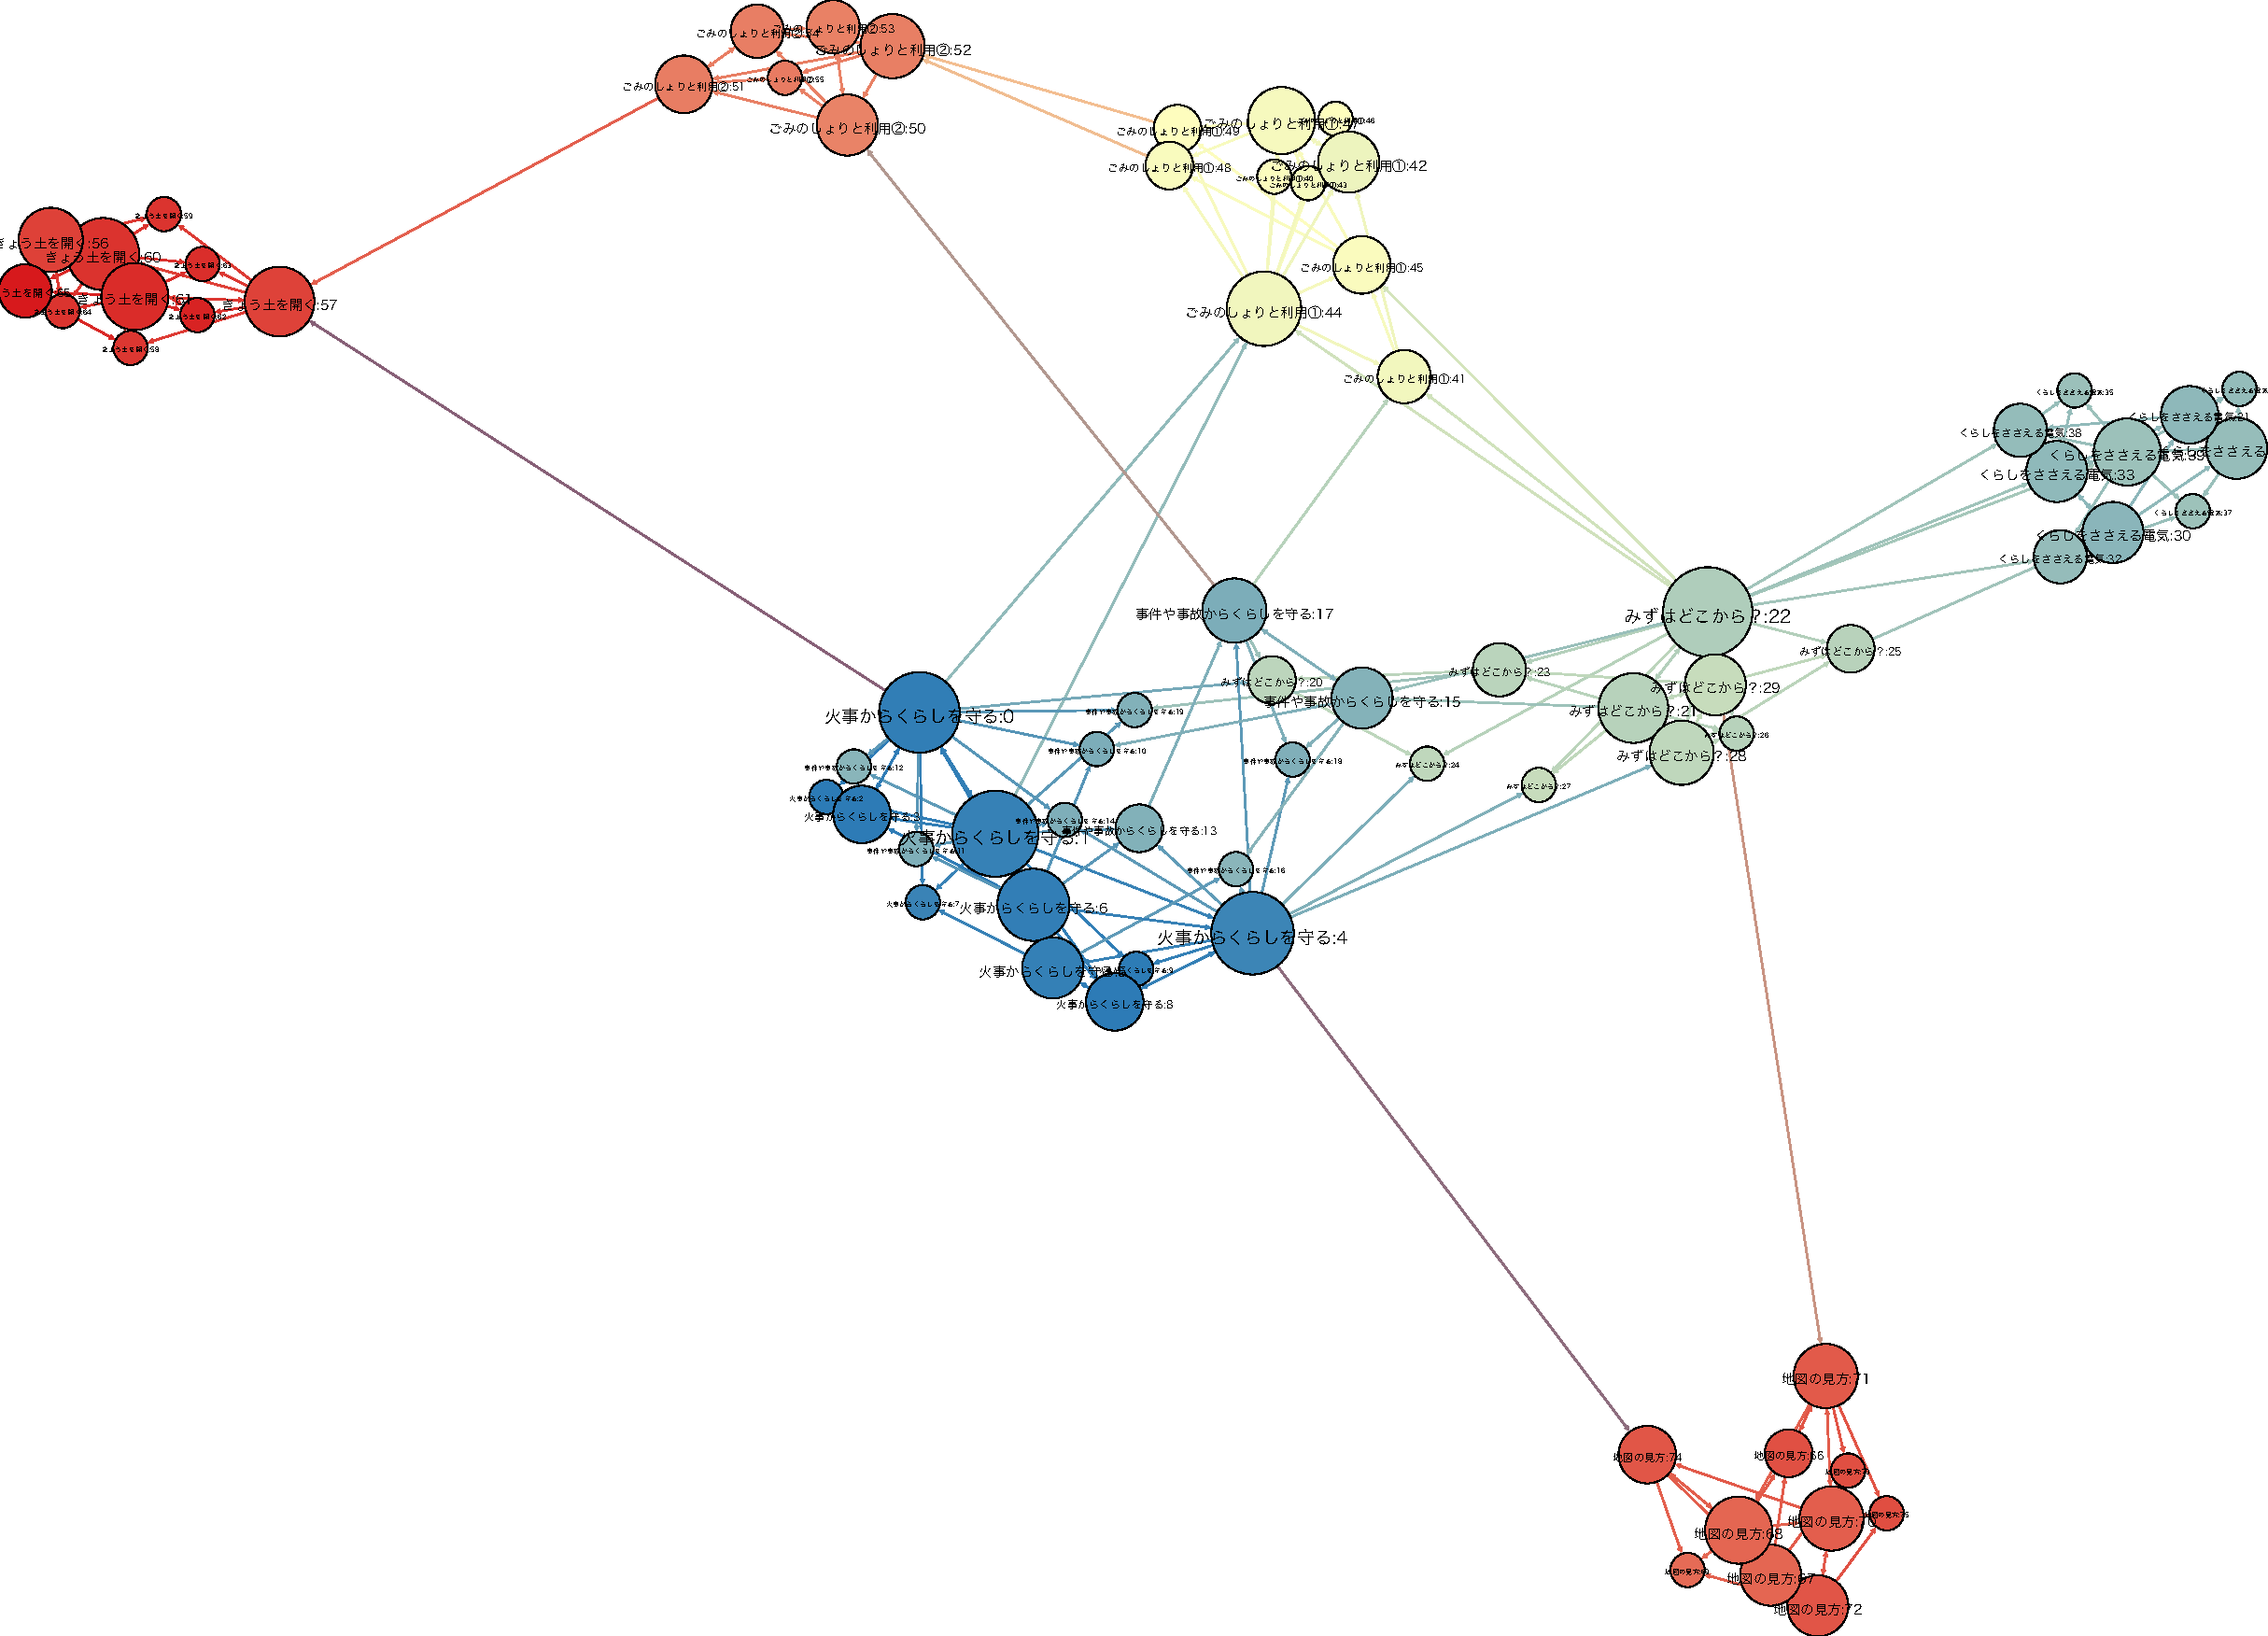
\includegraphics[width=200pt, height=200pt]{./img/net_s4soc.pdf}
			\caption{小学4年社会の問題間関係ネットワーク}
			\label{fig:net_s4soc}
		\endminipage\hfill
		\minipage{0.52\textwidth}
			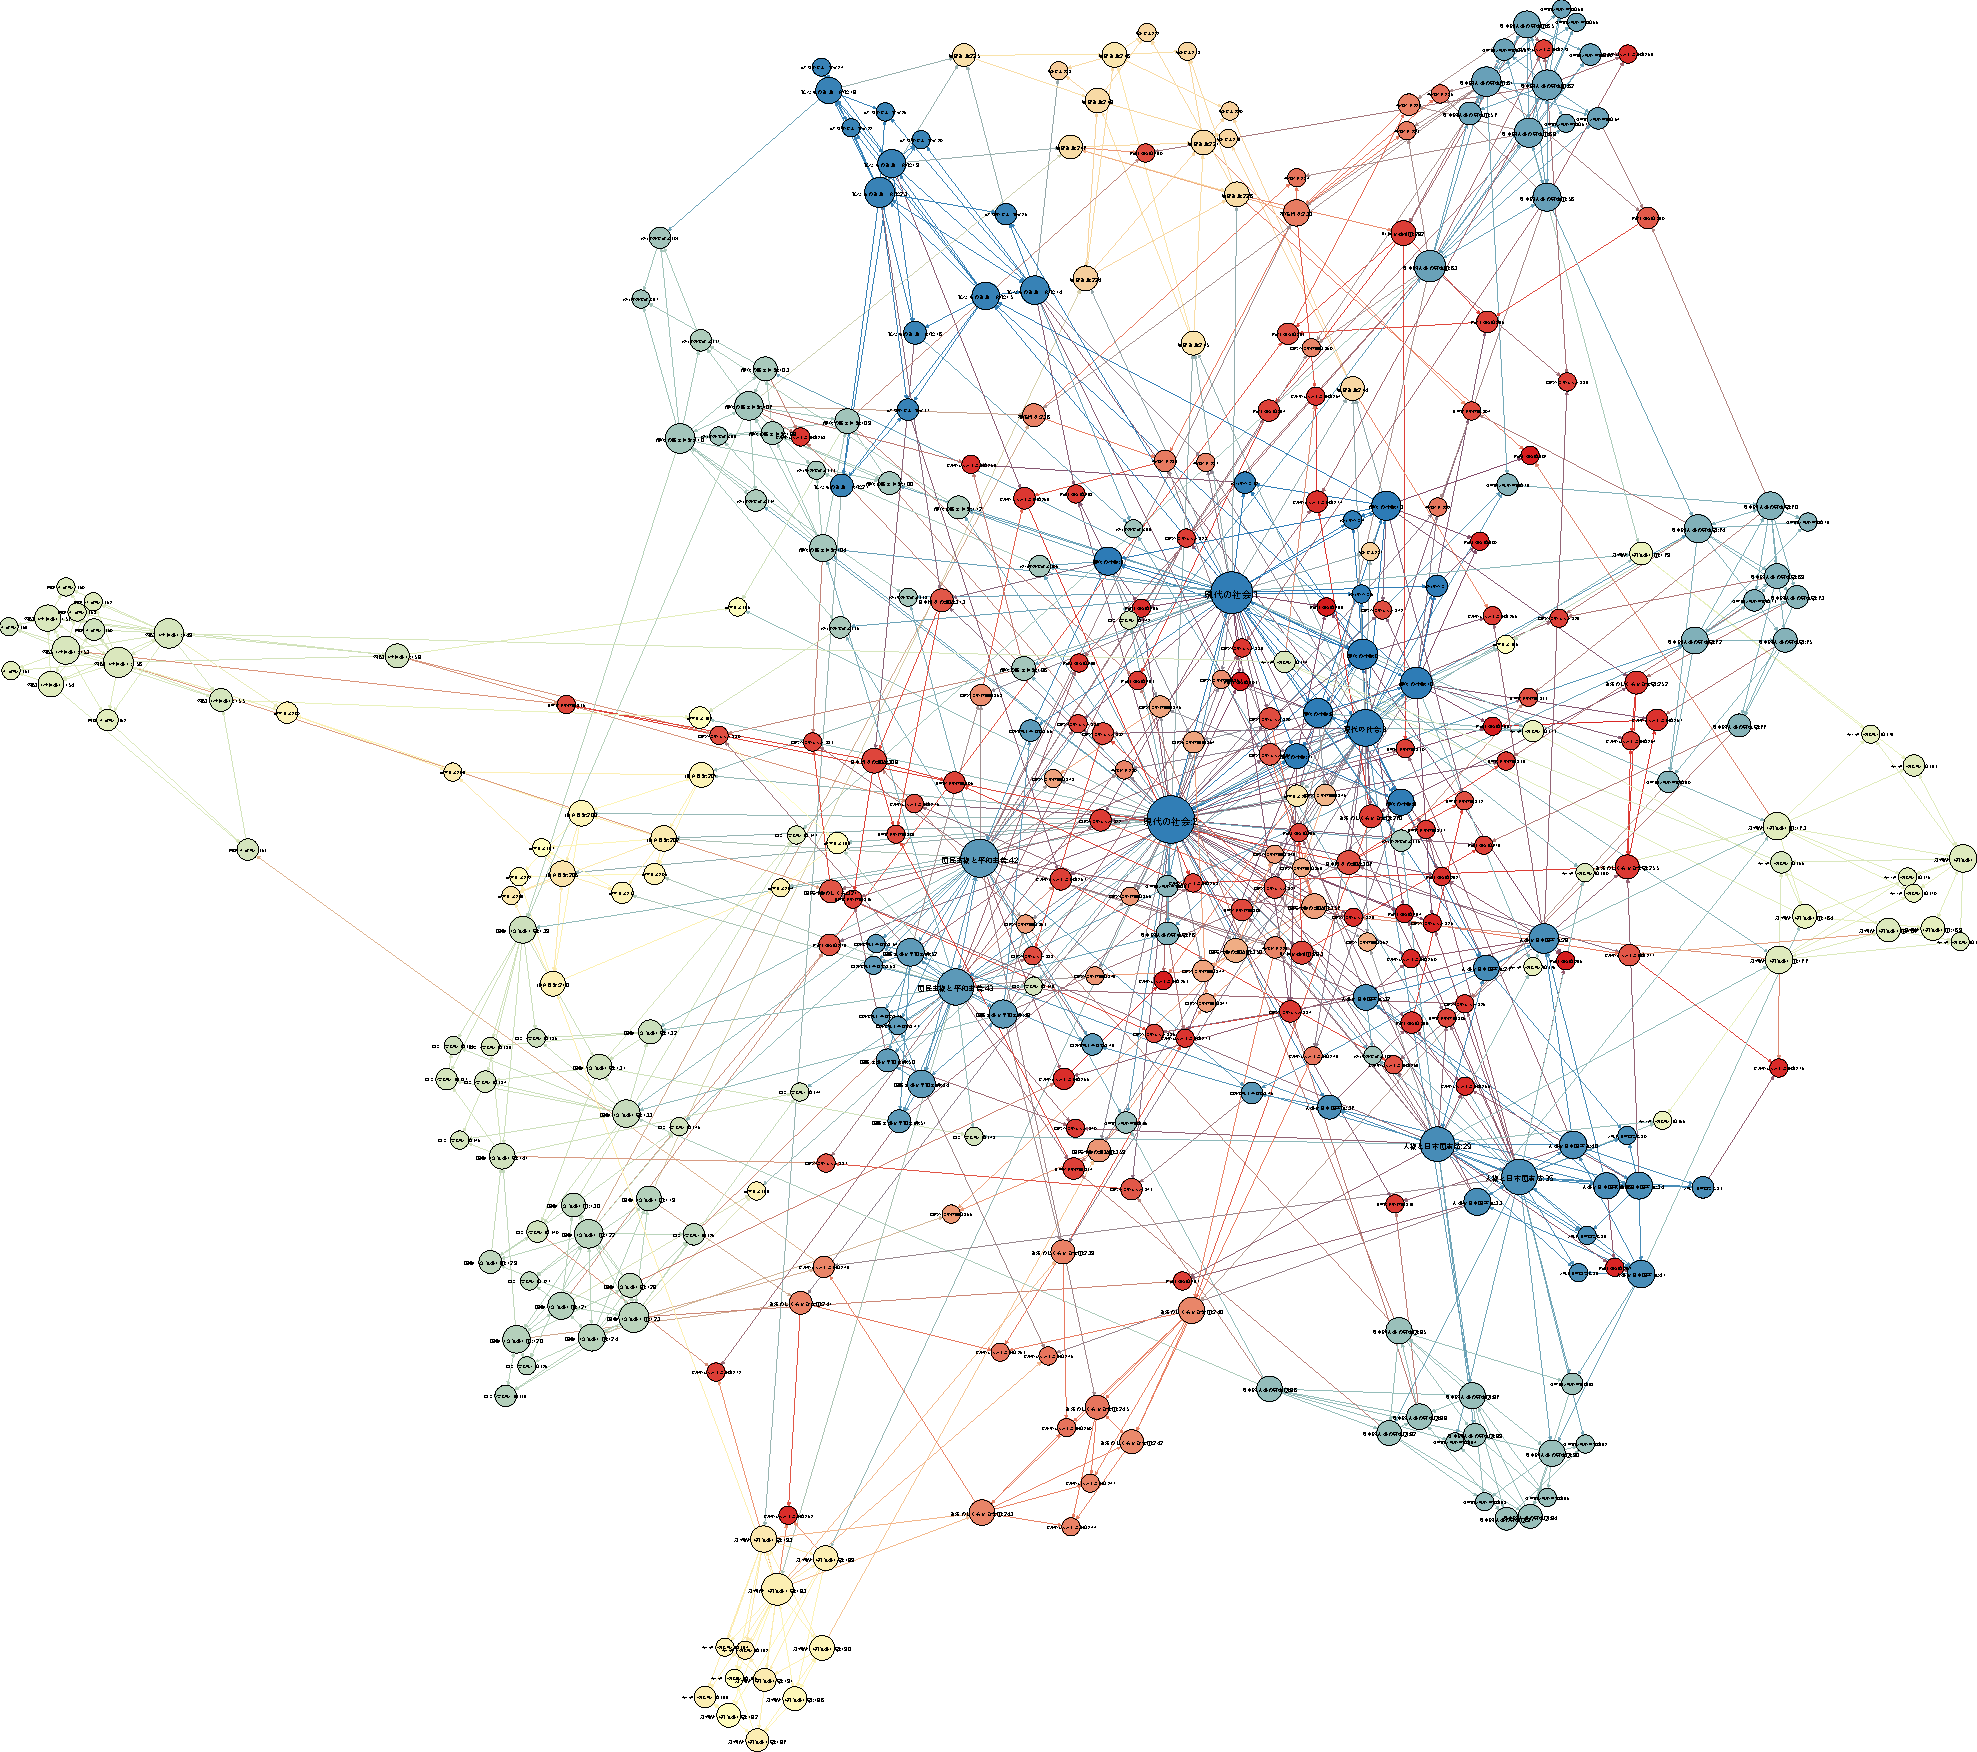
\includegraphics[width=200pt, height=200pt]{./img/net_c_cit.pdf}
			\caption{中学公民の問題間関係ネットワーク}
			\label{fig:net_c_cit}
		\endminipage\hfill
	}
	\hspace*{-10pt}\makebox[1.2\textwidth][c]{
		\minipage{0.52\textwidth}
			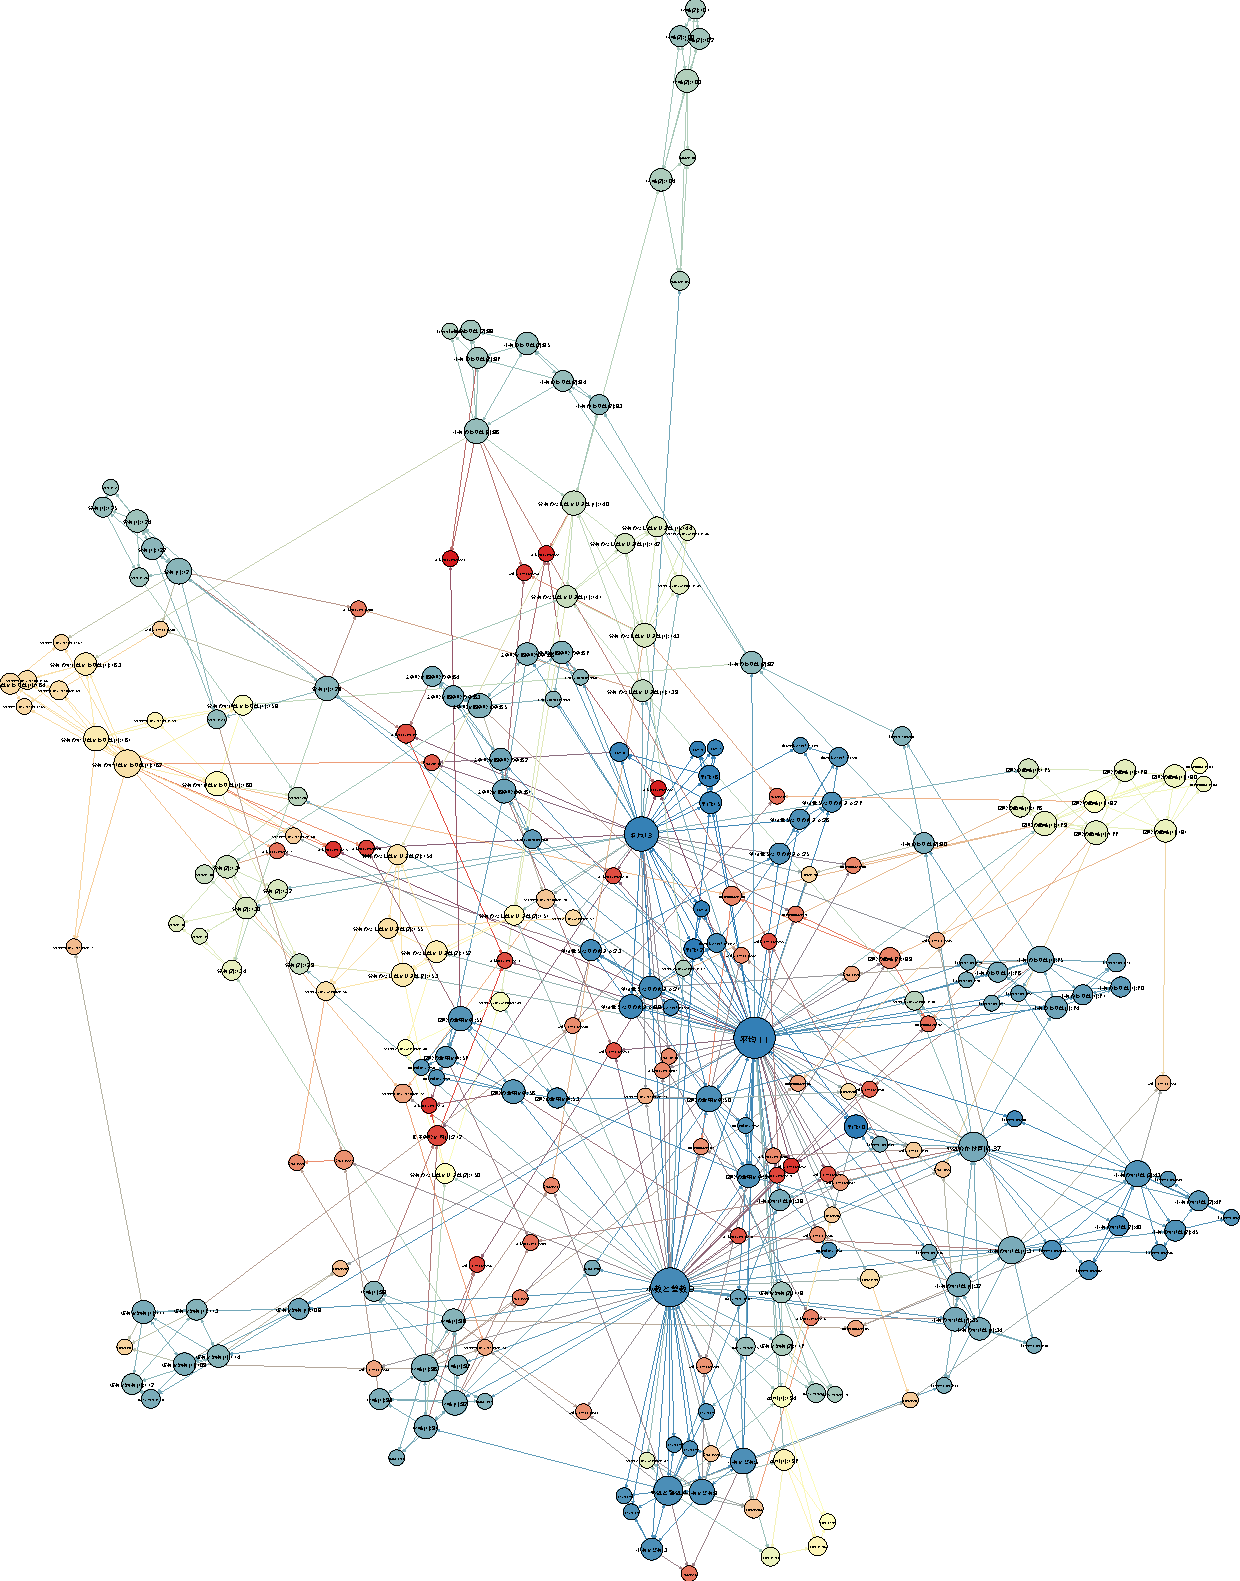
\includegraphics[width=200pt, height=200pt]{./img/net_s5mat.pdf}
			\caption{小学5年算数の問題間関係ネットワーク}
			\label{fig:net_s5_mat}
		\endminipage\hfill
		\minipage{0.52\textwidth}
			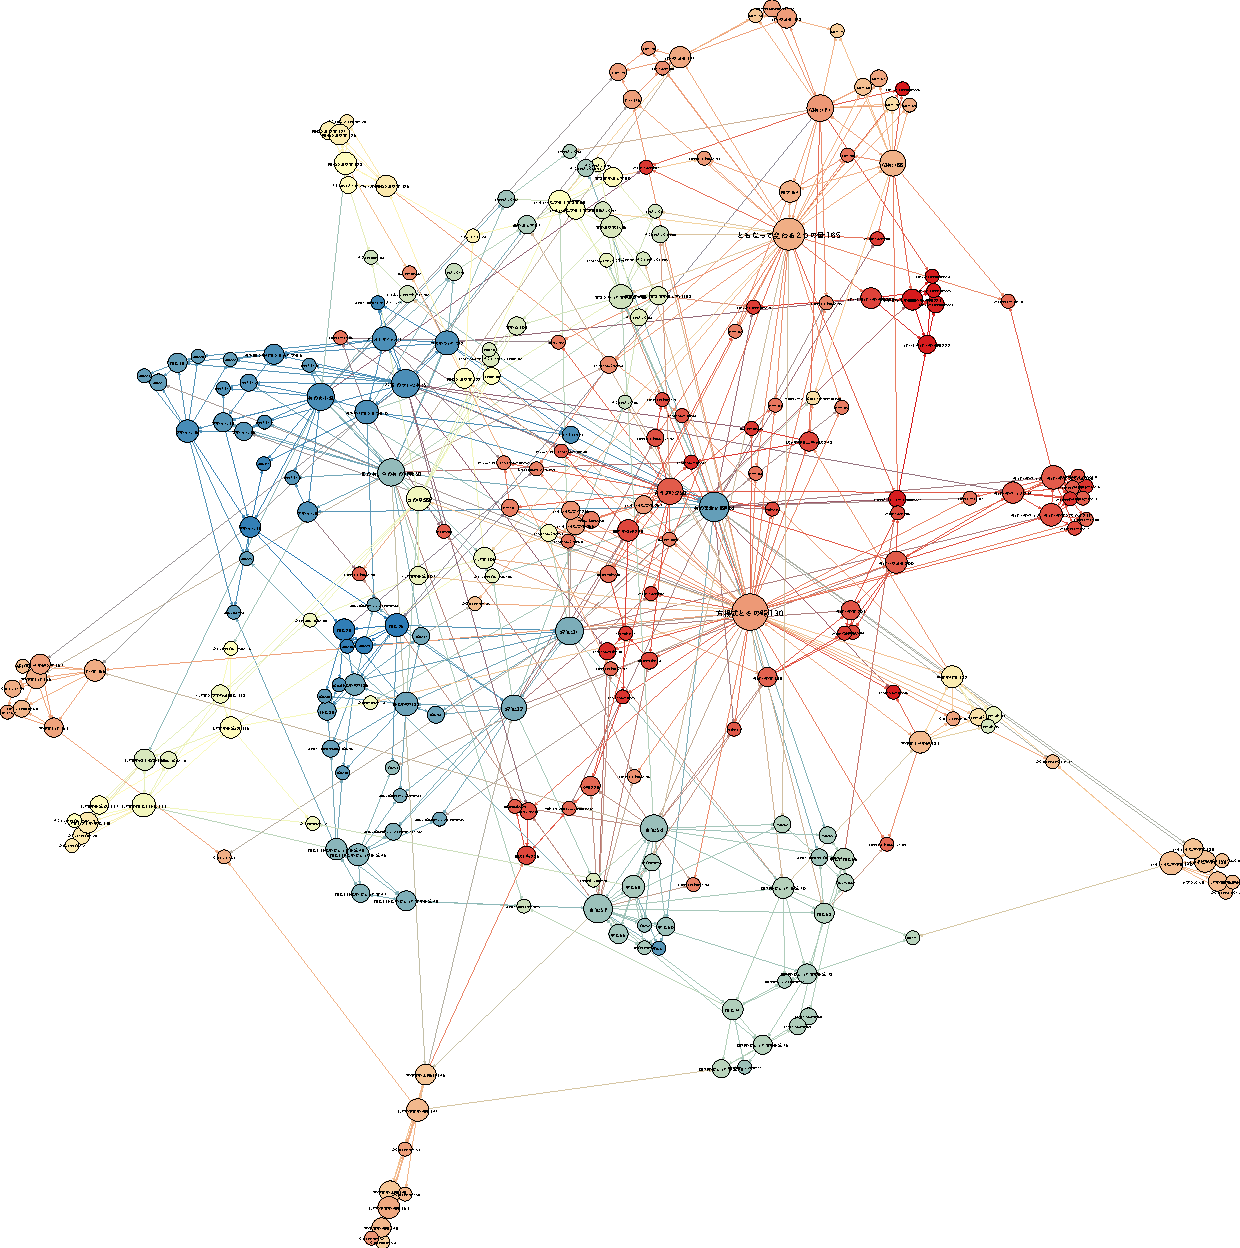
\includegraphics[width=200pt, height=200pt]{./img/net_c1mat.pdf}
			\caption{中学1年数学の問題間関係ネットワーク}
			\label{fig:net_c1mat}
		\endminipage\hfill
	}
\end{center}
\end{figure}

\begin{figure}[!htb]
\begin{center}
	\hspace*{-10pt}\makebox[1.2\textwidth][c]{
		\minipage{0.52\textwidth}
			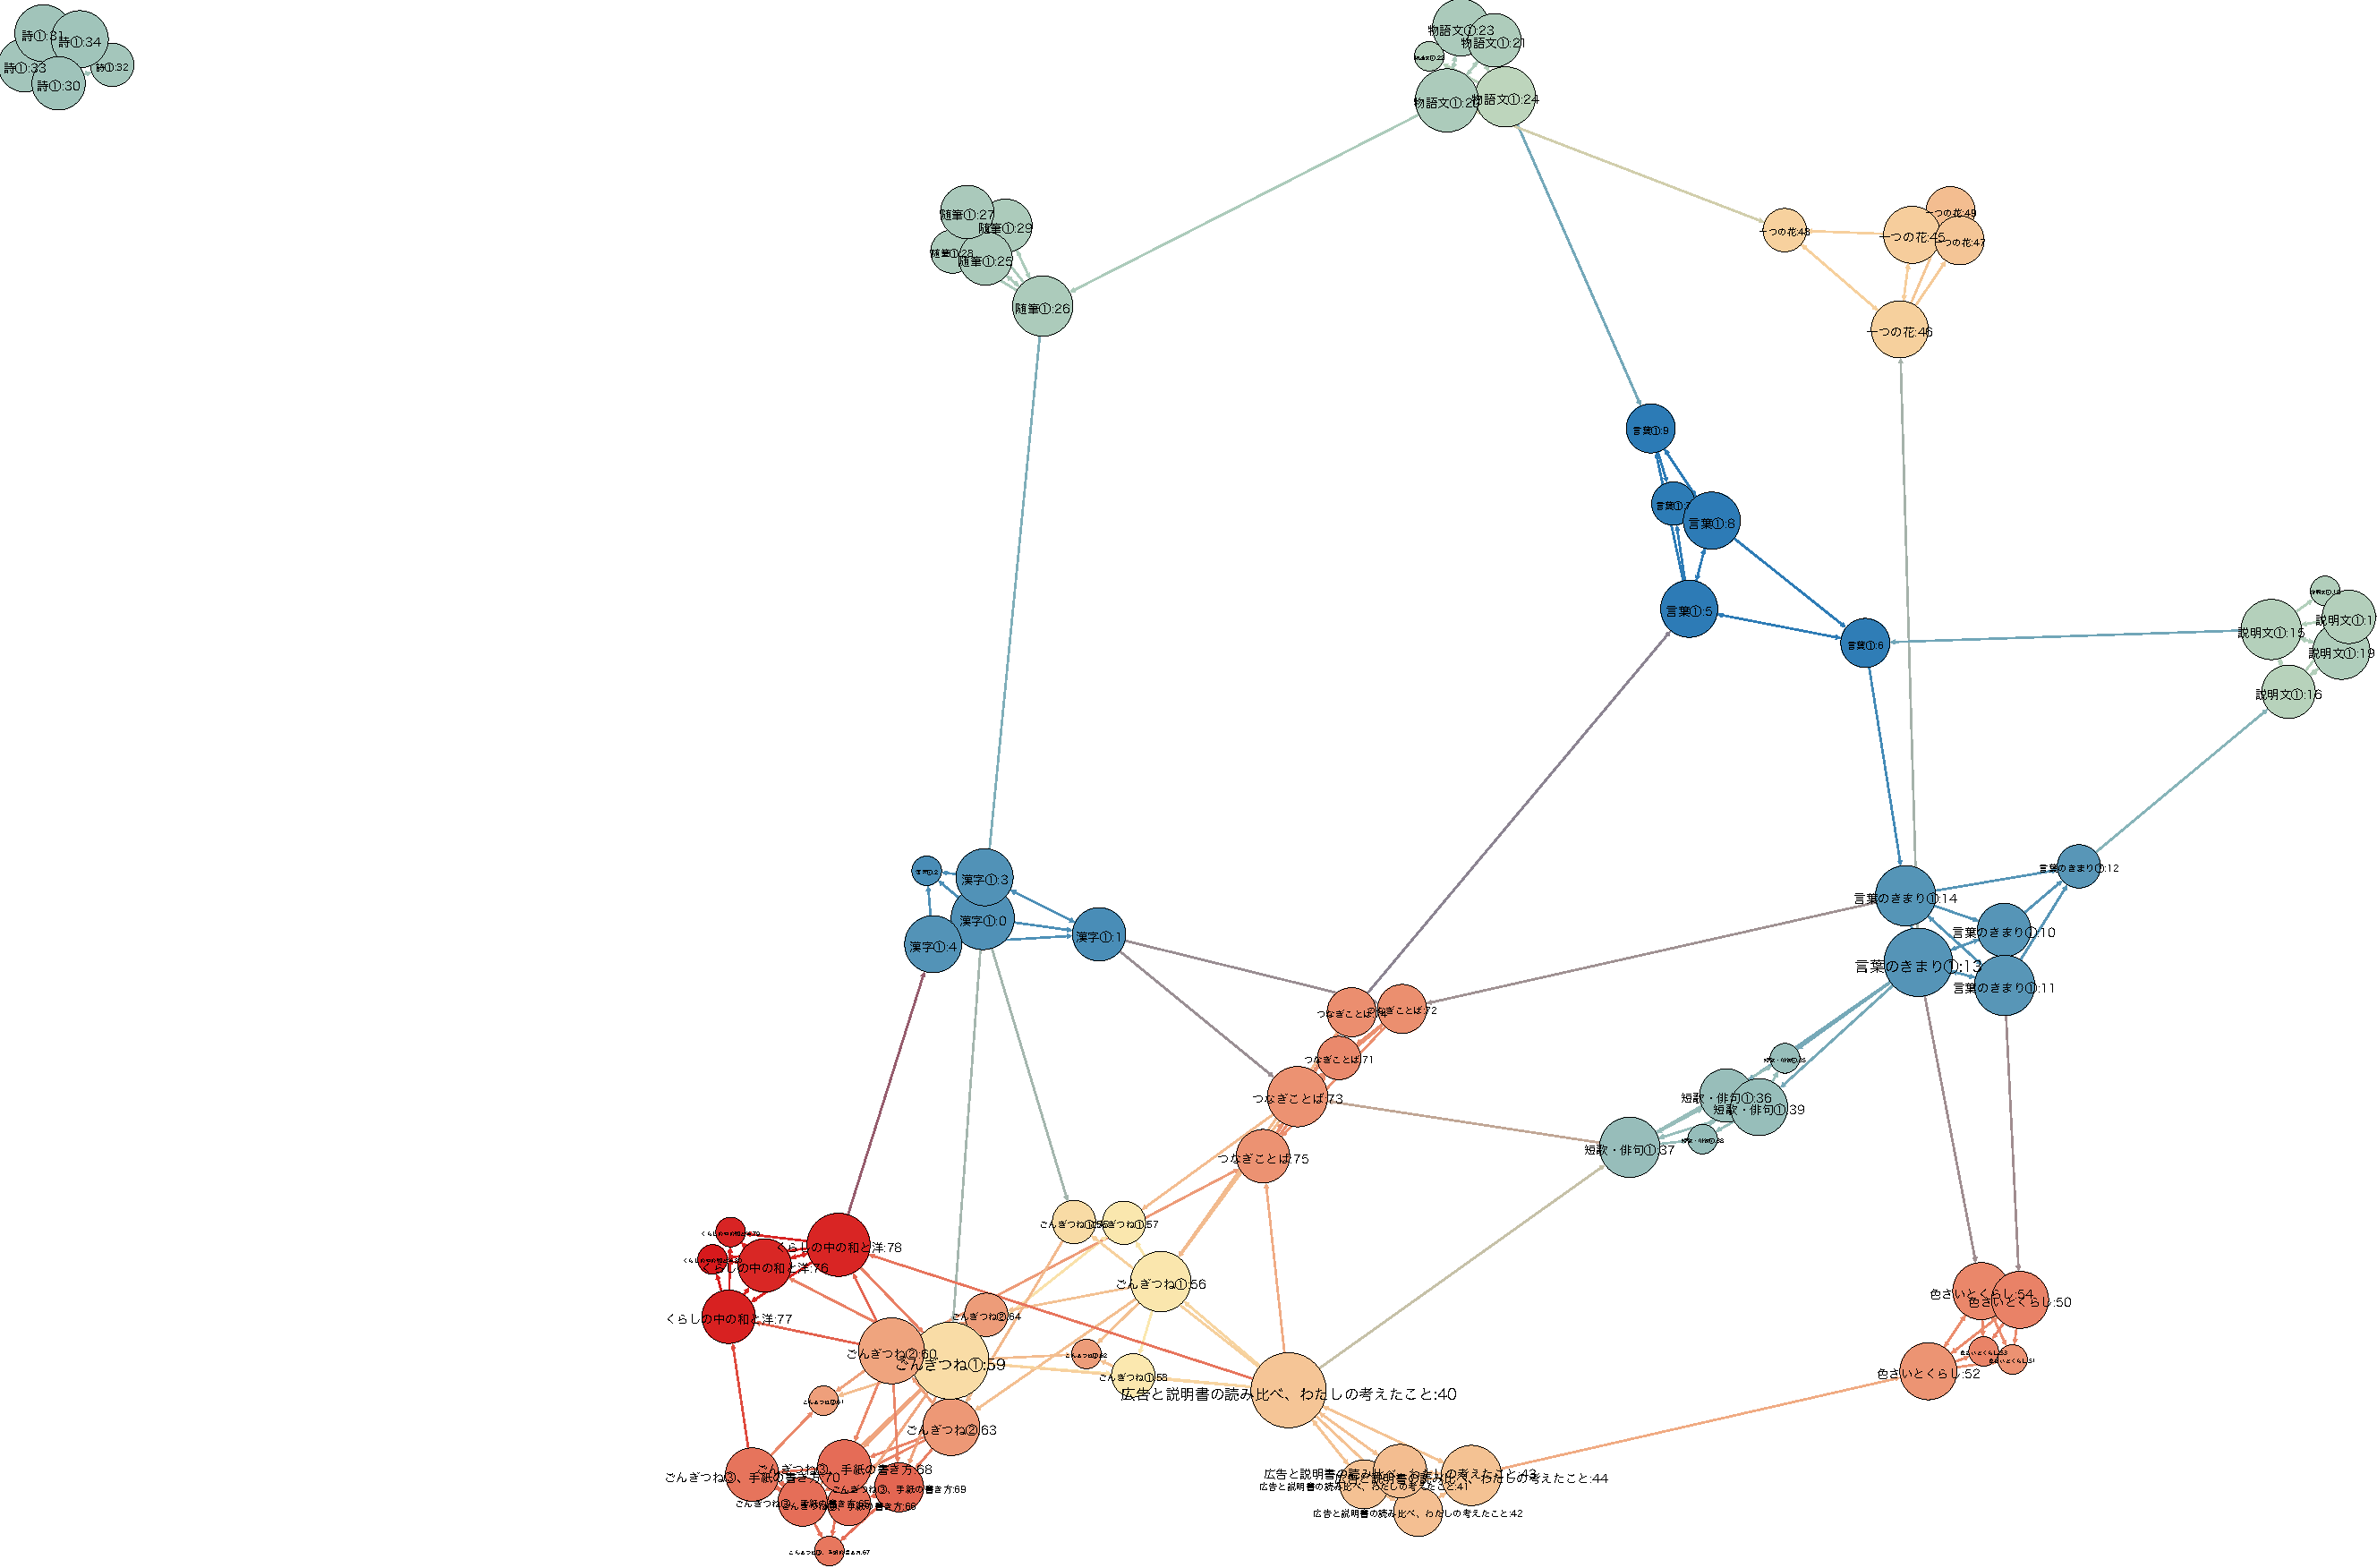
\includegraphics[width=200pt, height=200pt]{./img/net_s4jap.pdf}
			\caption{小学4年国語の問題間関係ネットワーク}
			\label{fig:net_s4_jap}
		\endminipage\hfill
		\minipage{0.52\textwidth}
			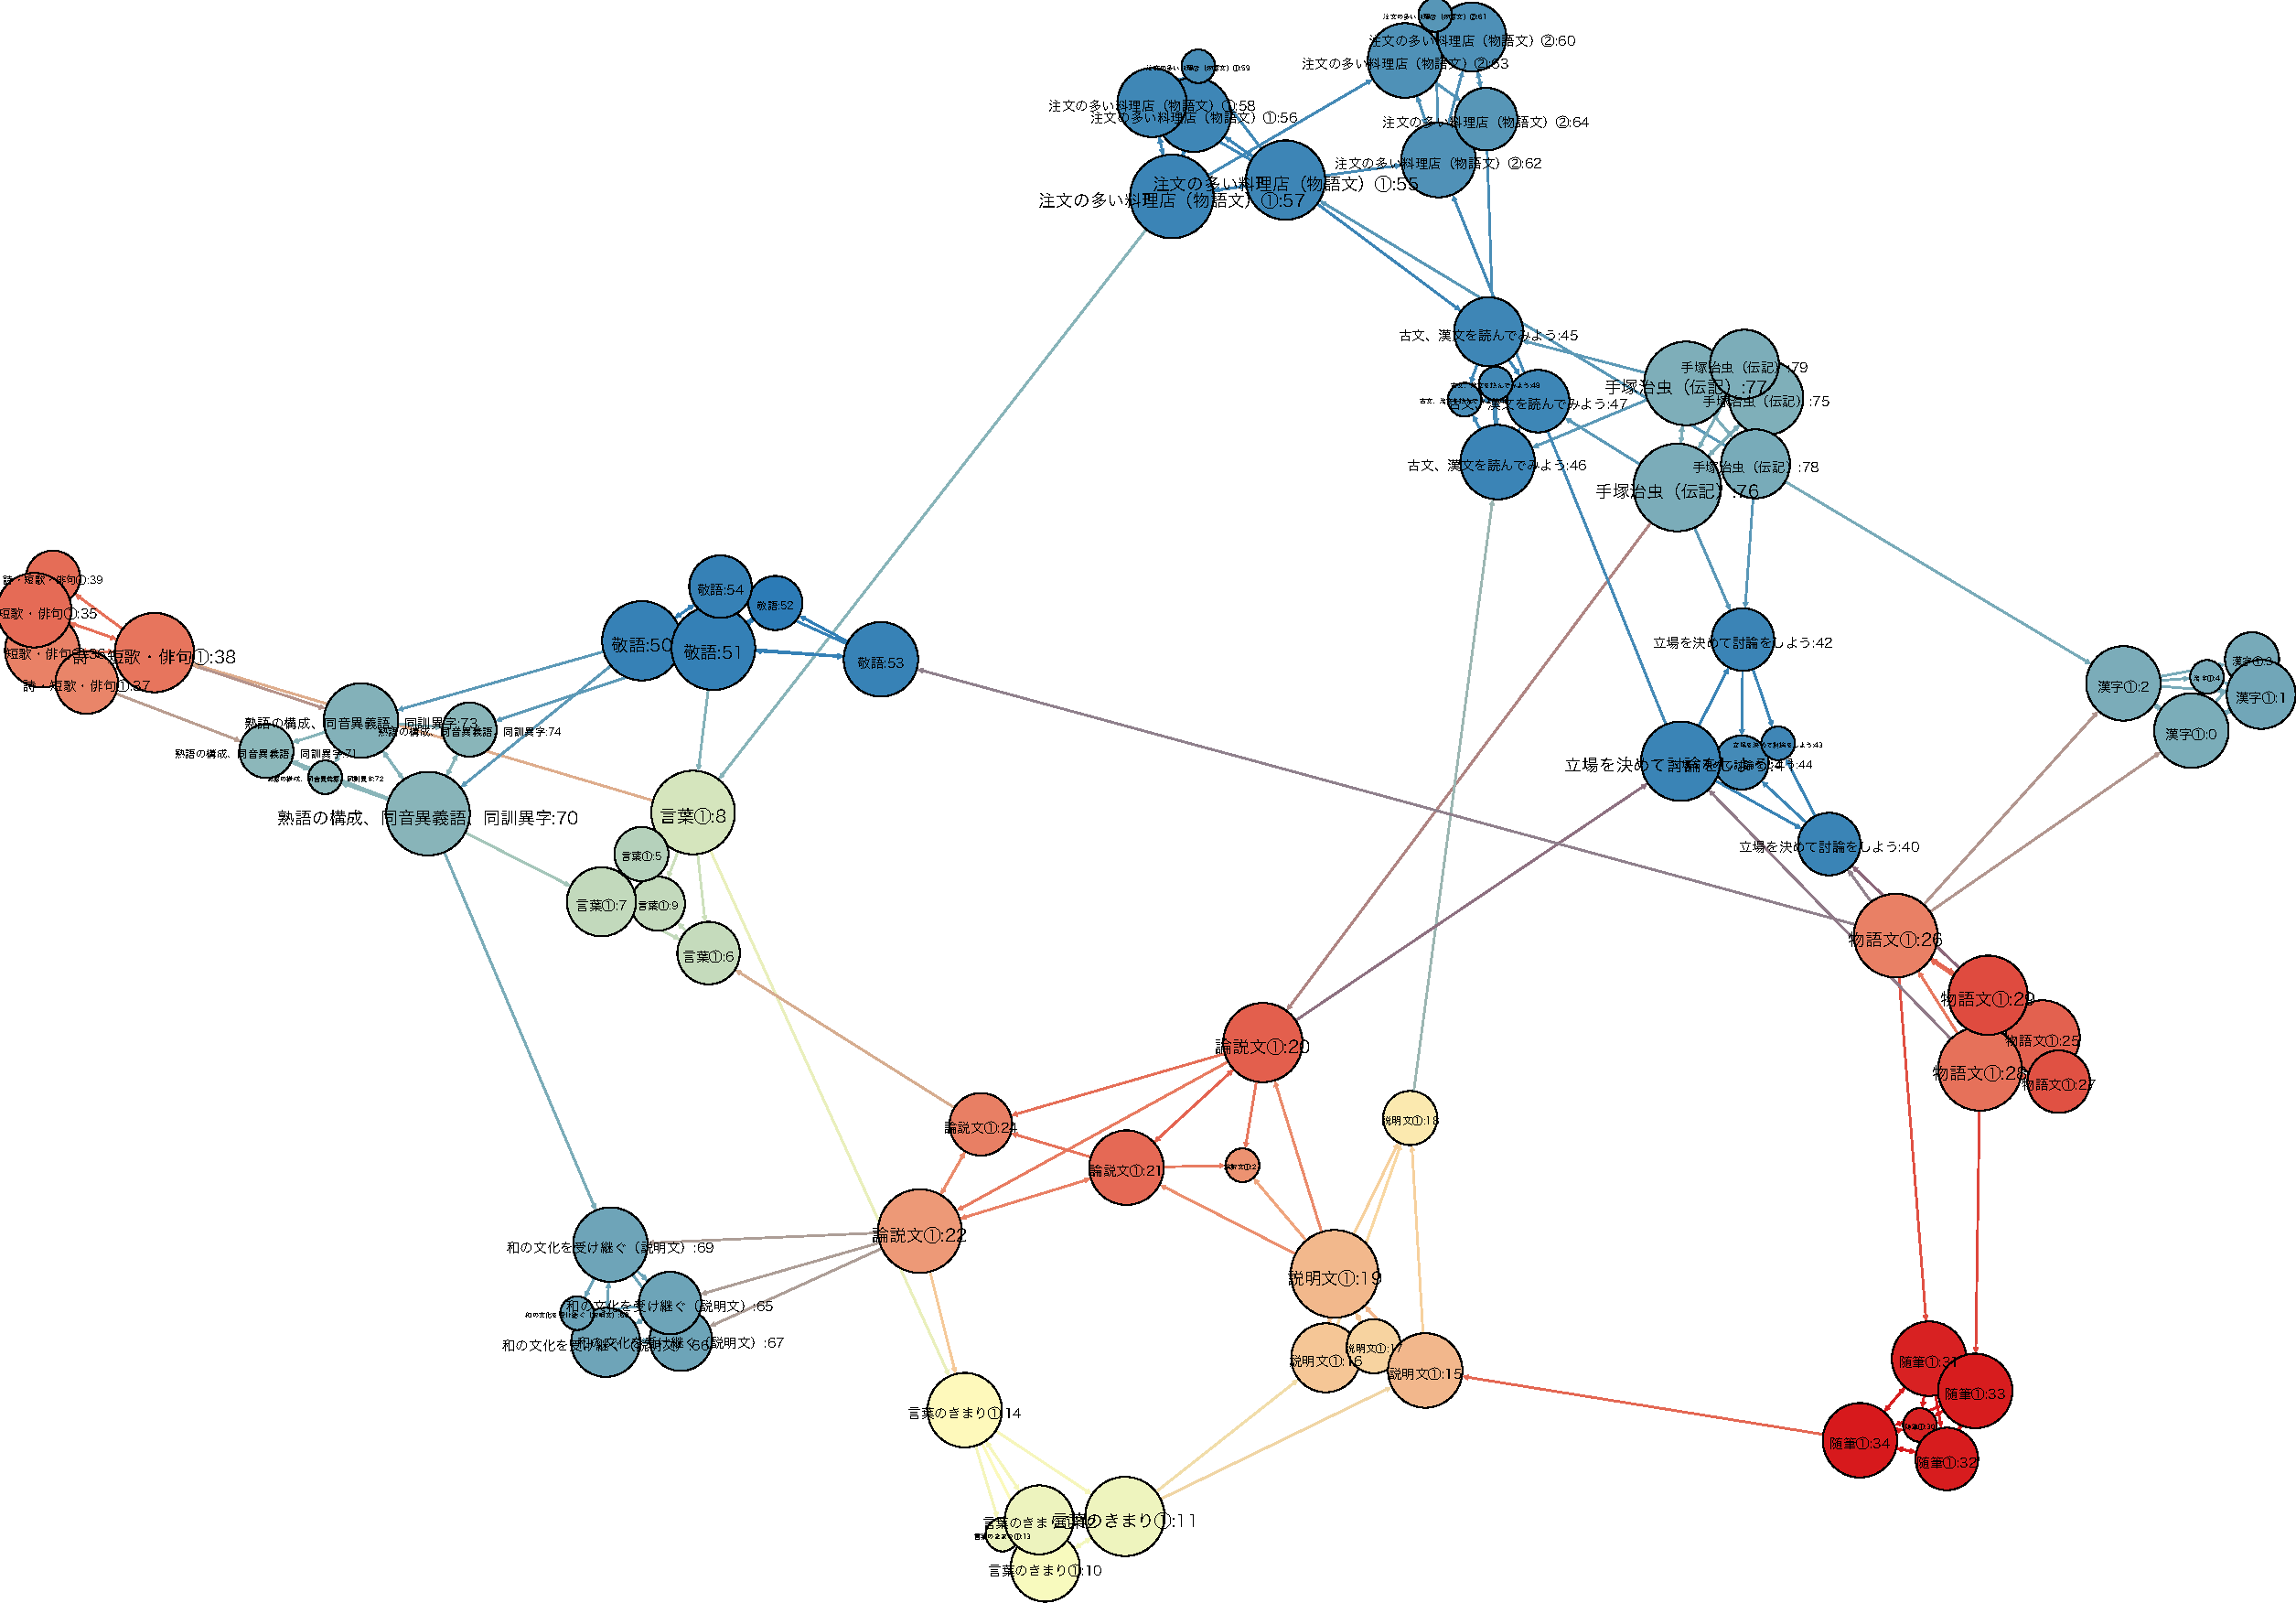
\includegraphics[width=200pt, height=200pt]{./img/net_s5jap.pdf}
			\caption{小学5年国語の問題間関係ネットワーク}
			\label{fig:net_s5_jap}
		\endminipage\hfill
	}
	\hspace*{-10pt}\makebox[1.2\textwidth][c]{
		\minipage{0.52\textwidth}
			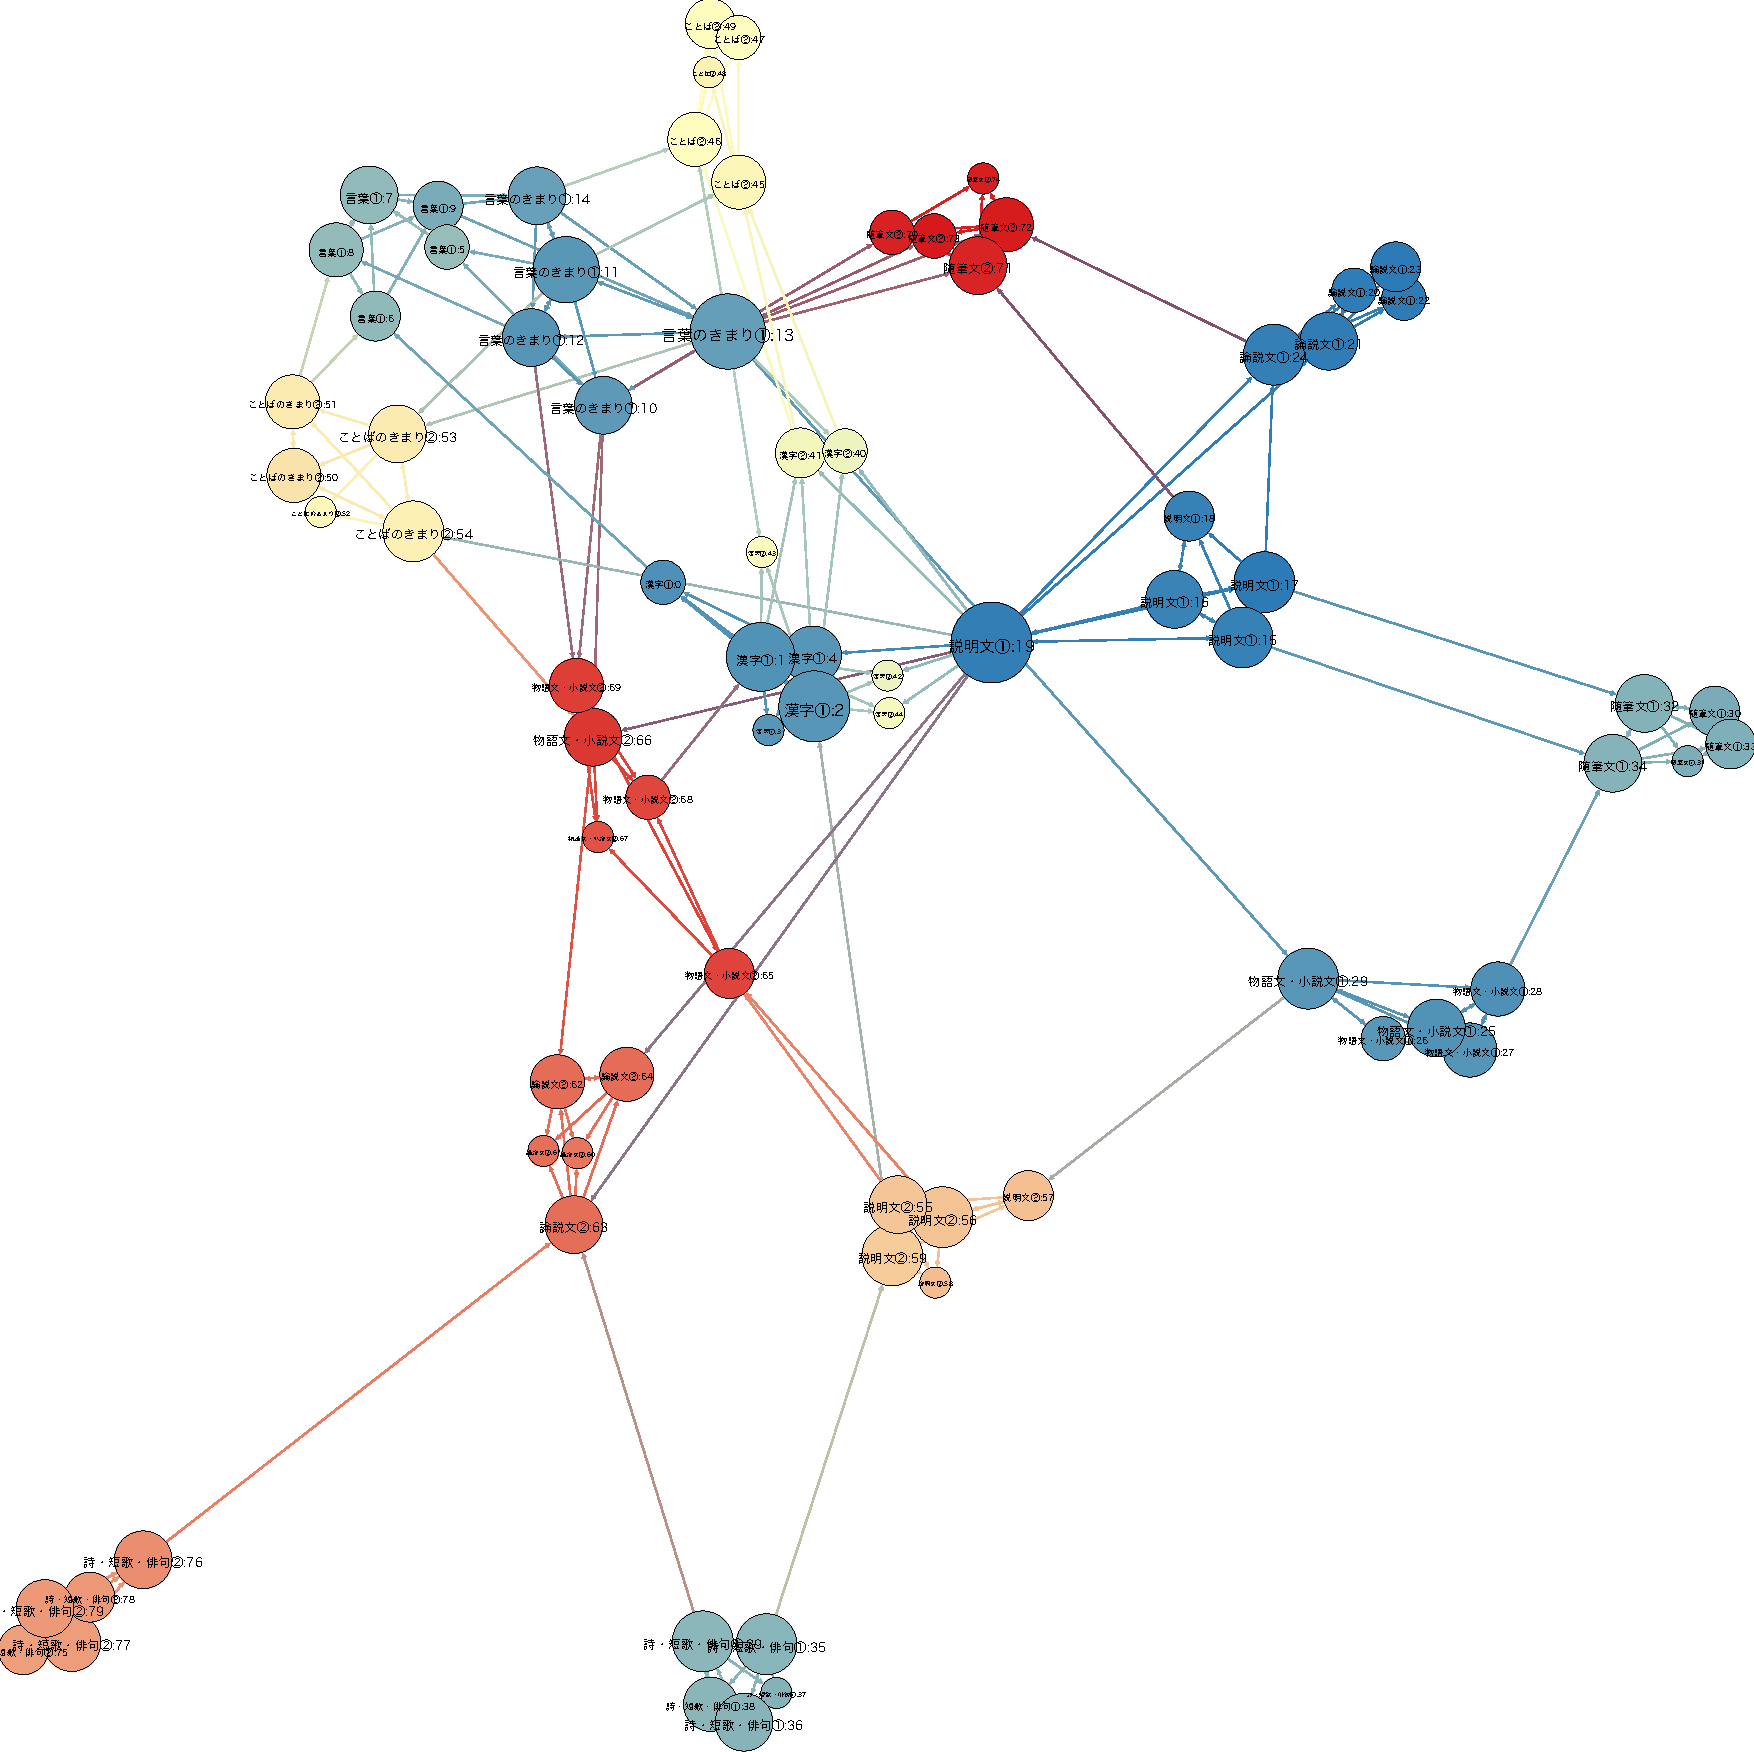
\includegraphics[width=200pt, height=200pt]{./img/net_s6jap.pdf}
			\caption{小学6年国語の問題間関係ネットワーク}
			\label{fig:net_s6_jap}
		\endminipage\hfill
		\minipage{0.52\textwidth}
			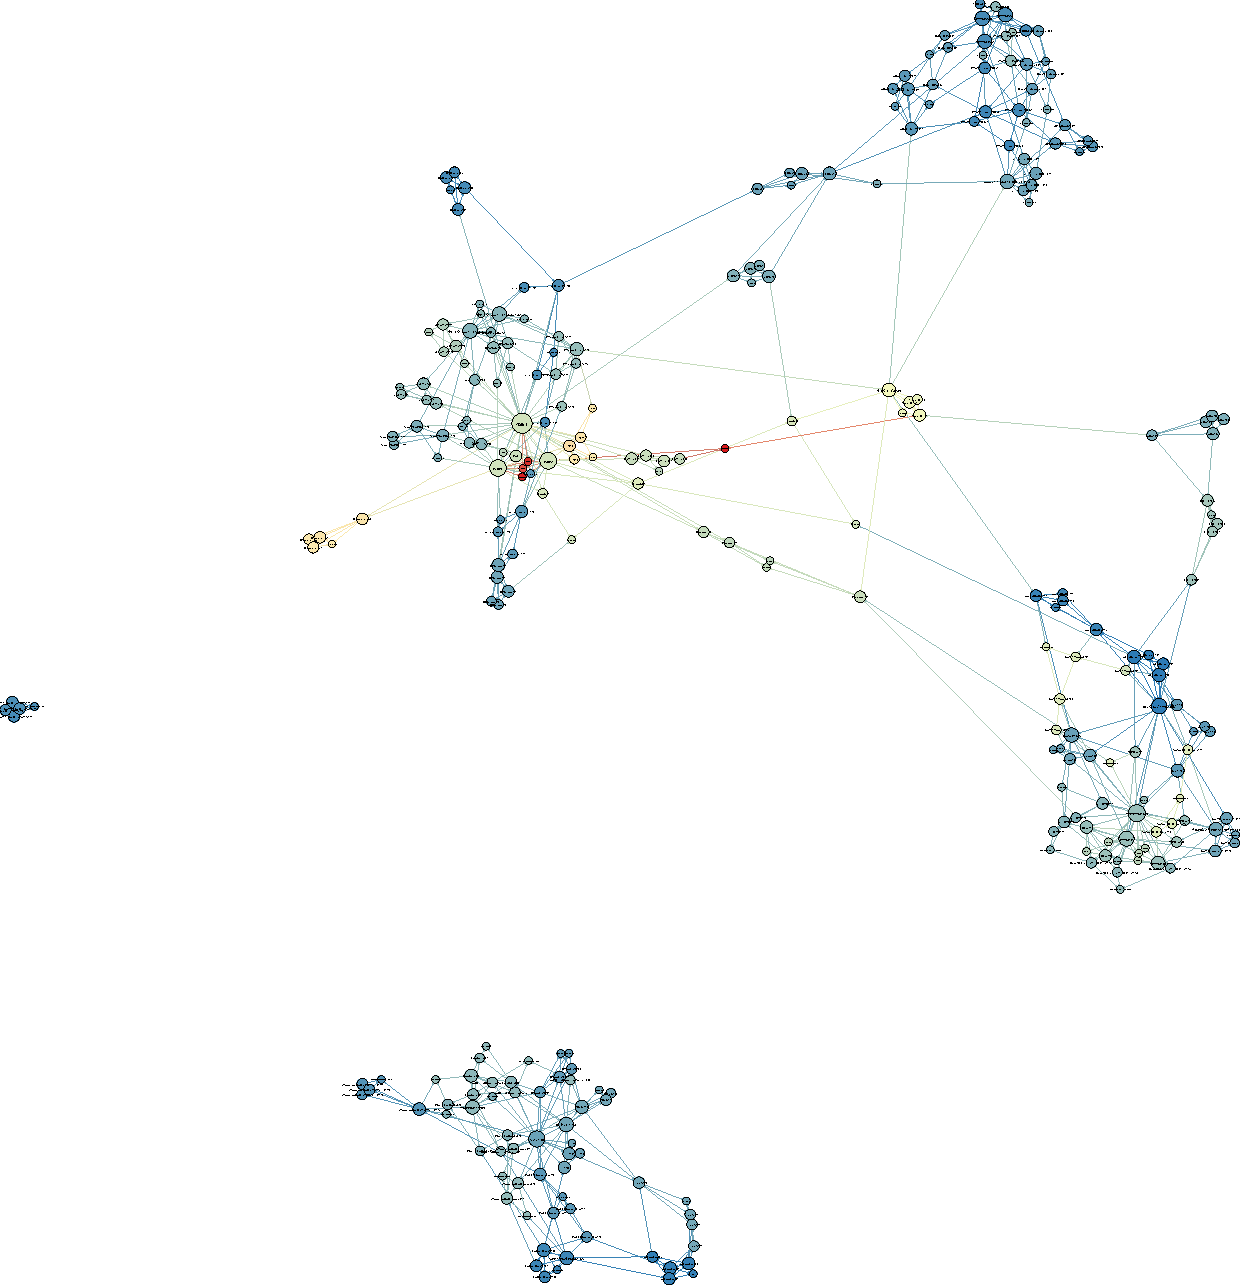
\includegraphics[width=200pt, height=200pt]{./img/net_c1jap.pdf}
			\caption{中学1年国語の問題間関係ネットワーク}
			\label{fig:net_c1jap}
		\endminipage\hfill
	}
\end{center}
\end{figure}


\begin{figure}[!htb]
\begin{center}
	\hspace*{-10pt}\makebox[1.2\textwidth][c]{
		\minipage{0.52\textwidth}
			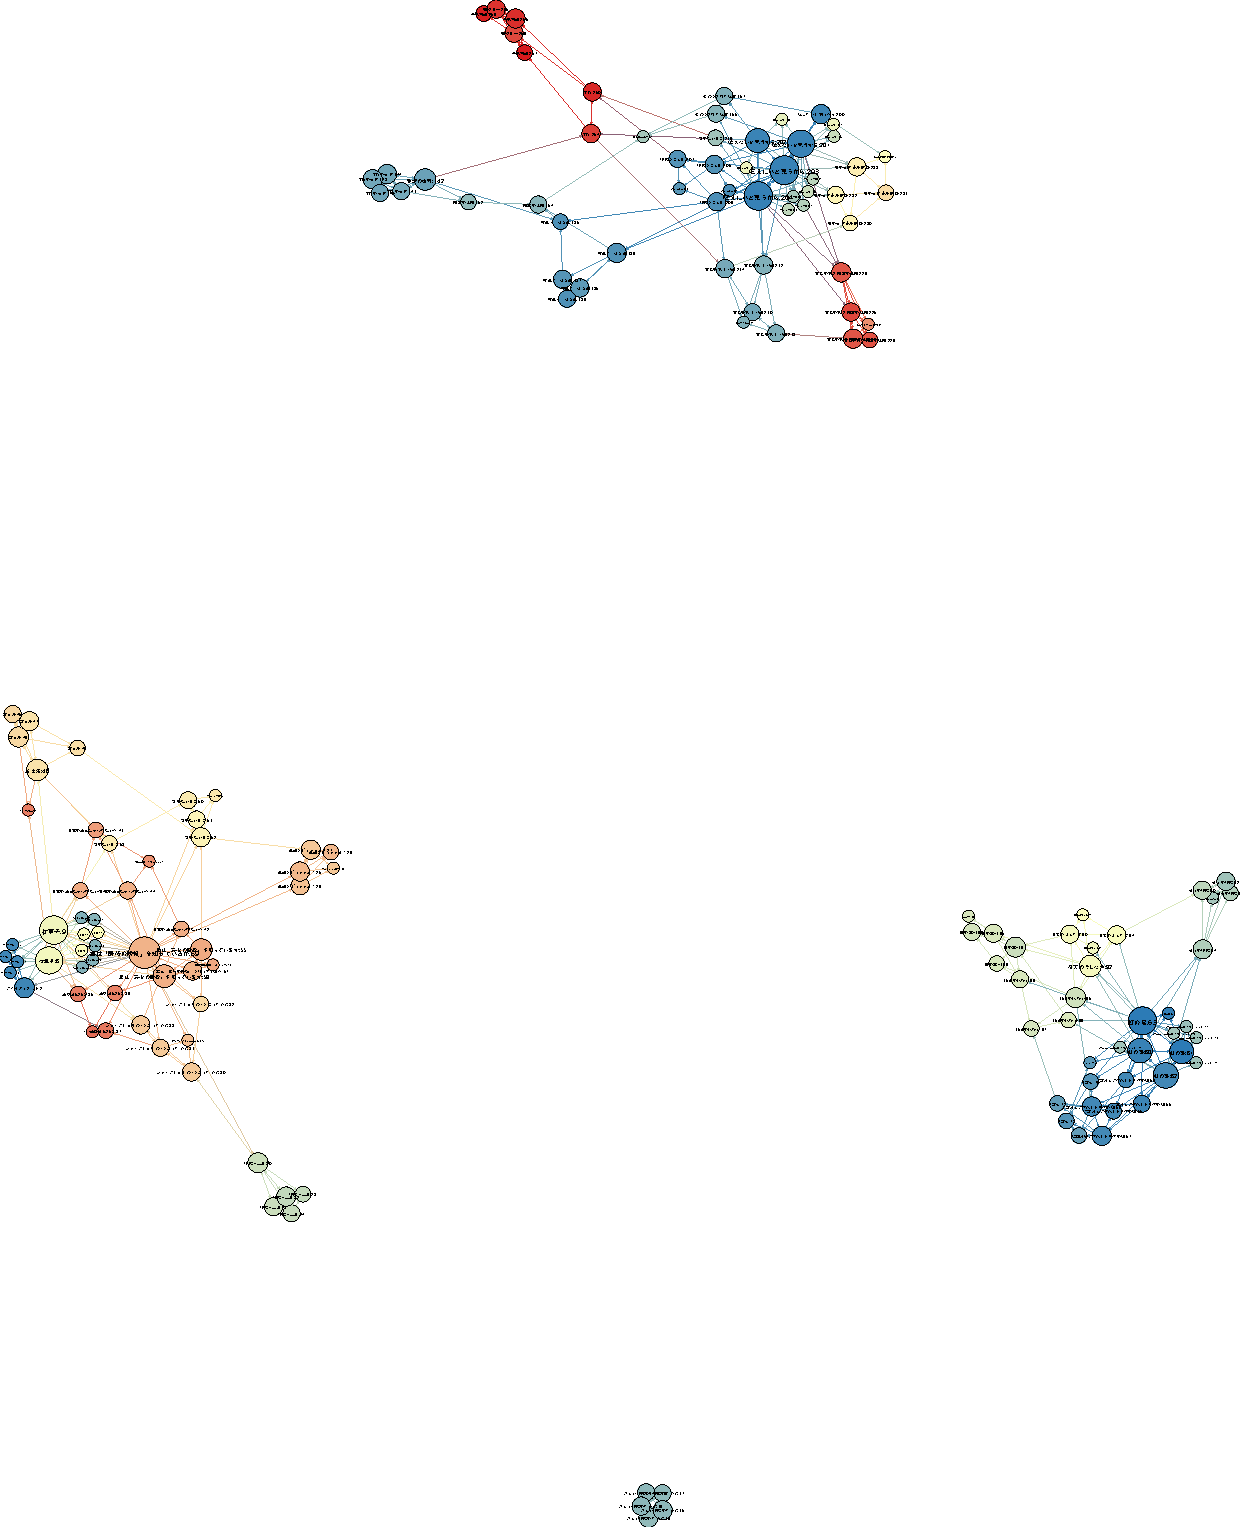
\includegraphics[width=200pt, height=200pt]{./img/net_c2jap.pdf}
			\caption{中学2年国語の問題間関係ネットワーク}
			\label{fig:net_c2jap}
		\endminipage\hfill
		\minipage{0.52\textwidth}
			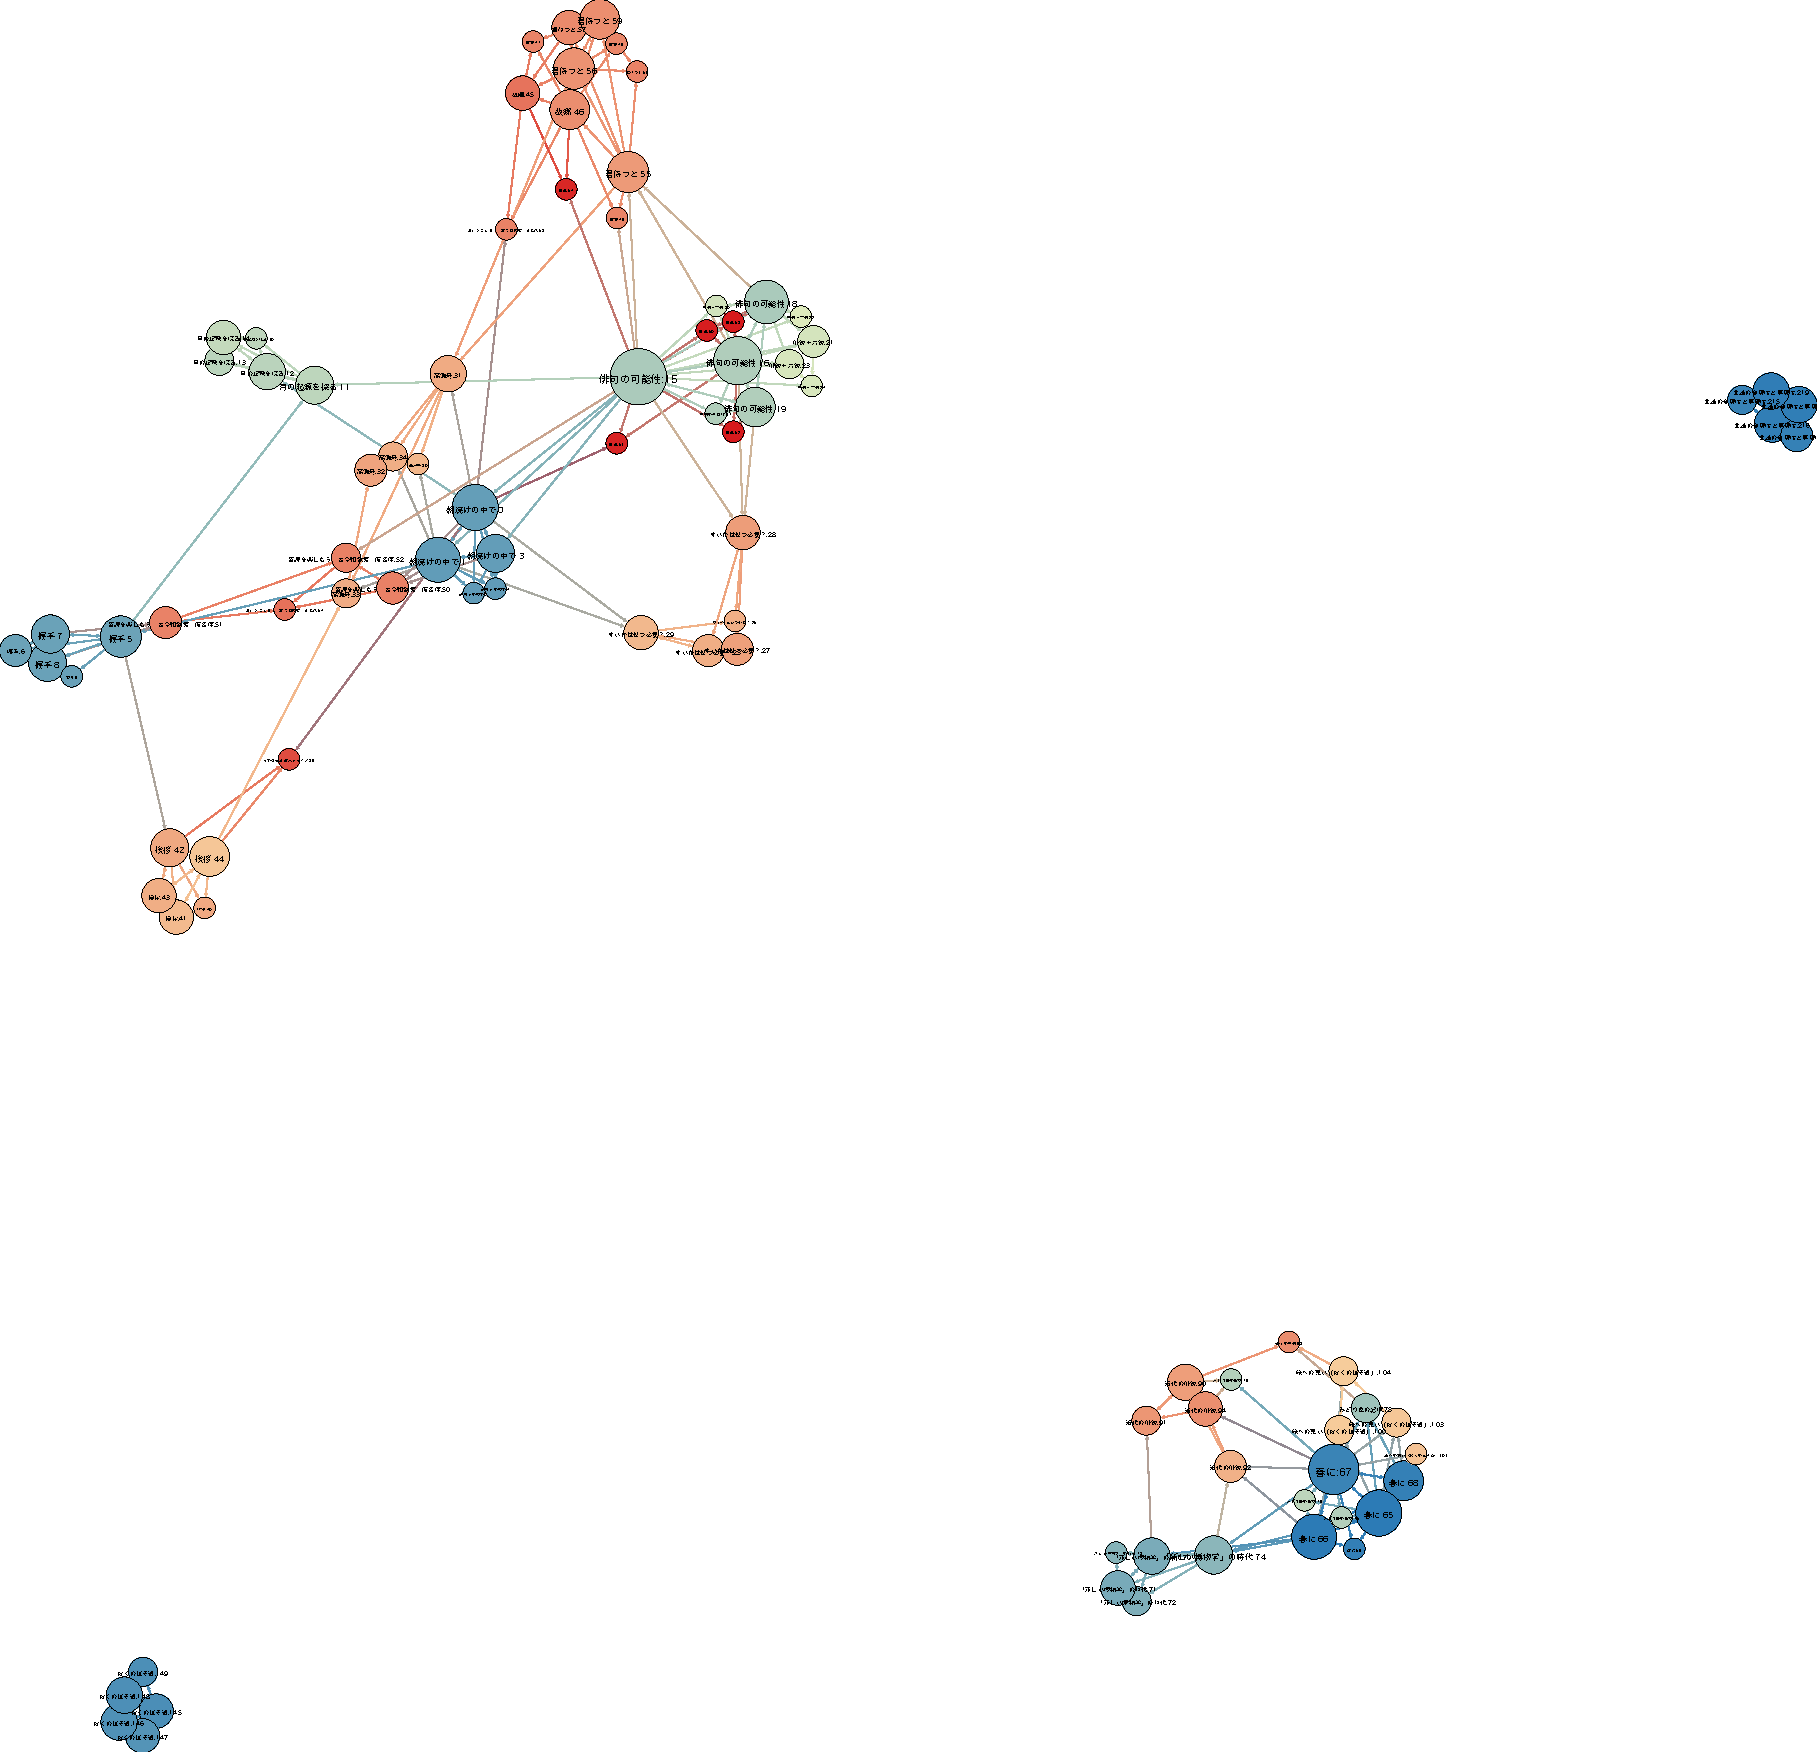
\includegraphics[width=200pt, height=200pt]{./img/net_c3jap.pdf}
			\caption{中学3年国語の問題間関係ネットワーク}
			\label{fig:net_c3jap}
		\endminipage\hfill
	}
	\hspace*{-10pt}\makebox[1.2\textwidth][c]{
		\minipage{0.52\textwidth}
			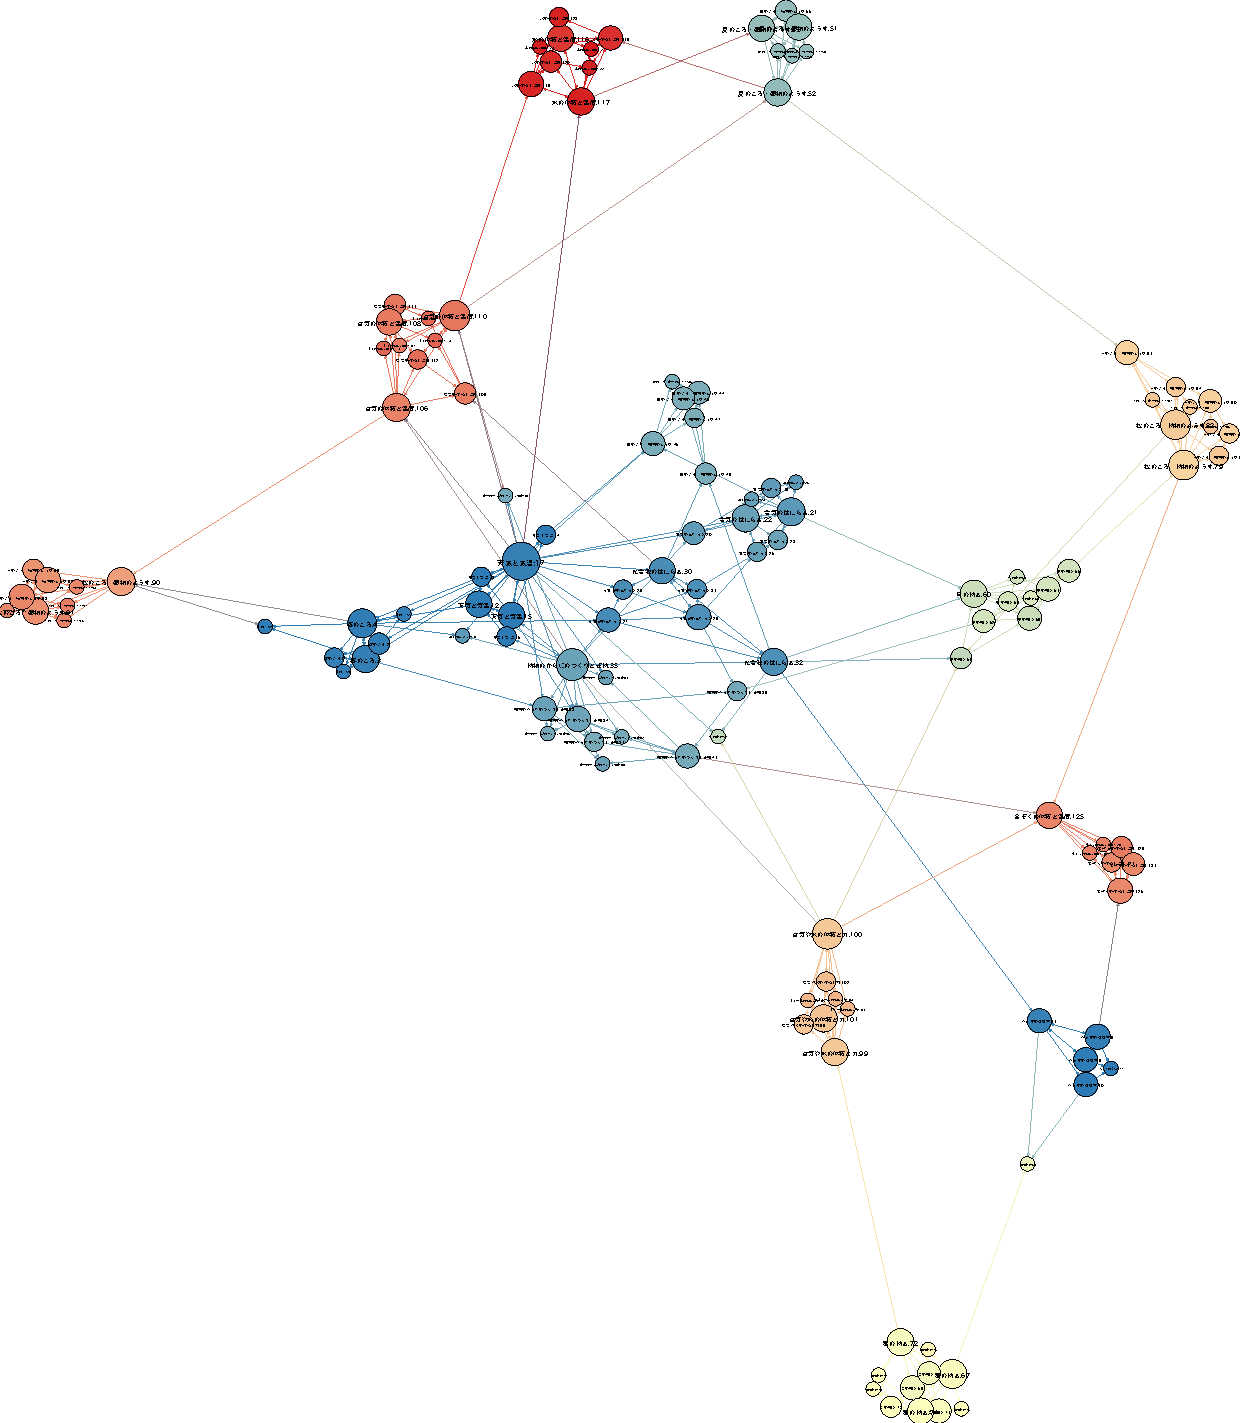
\includegraphics[width=200pt, height=200pt]{./img/net_s4sci.pdf}
			\caption{小学4年理科の問題間関係ネットワーク}
			\label{fig:net_s4sci}
		\endminipage\hfill
		\minipage{0.52\textwidth}
			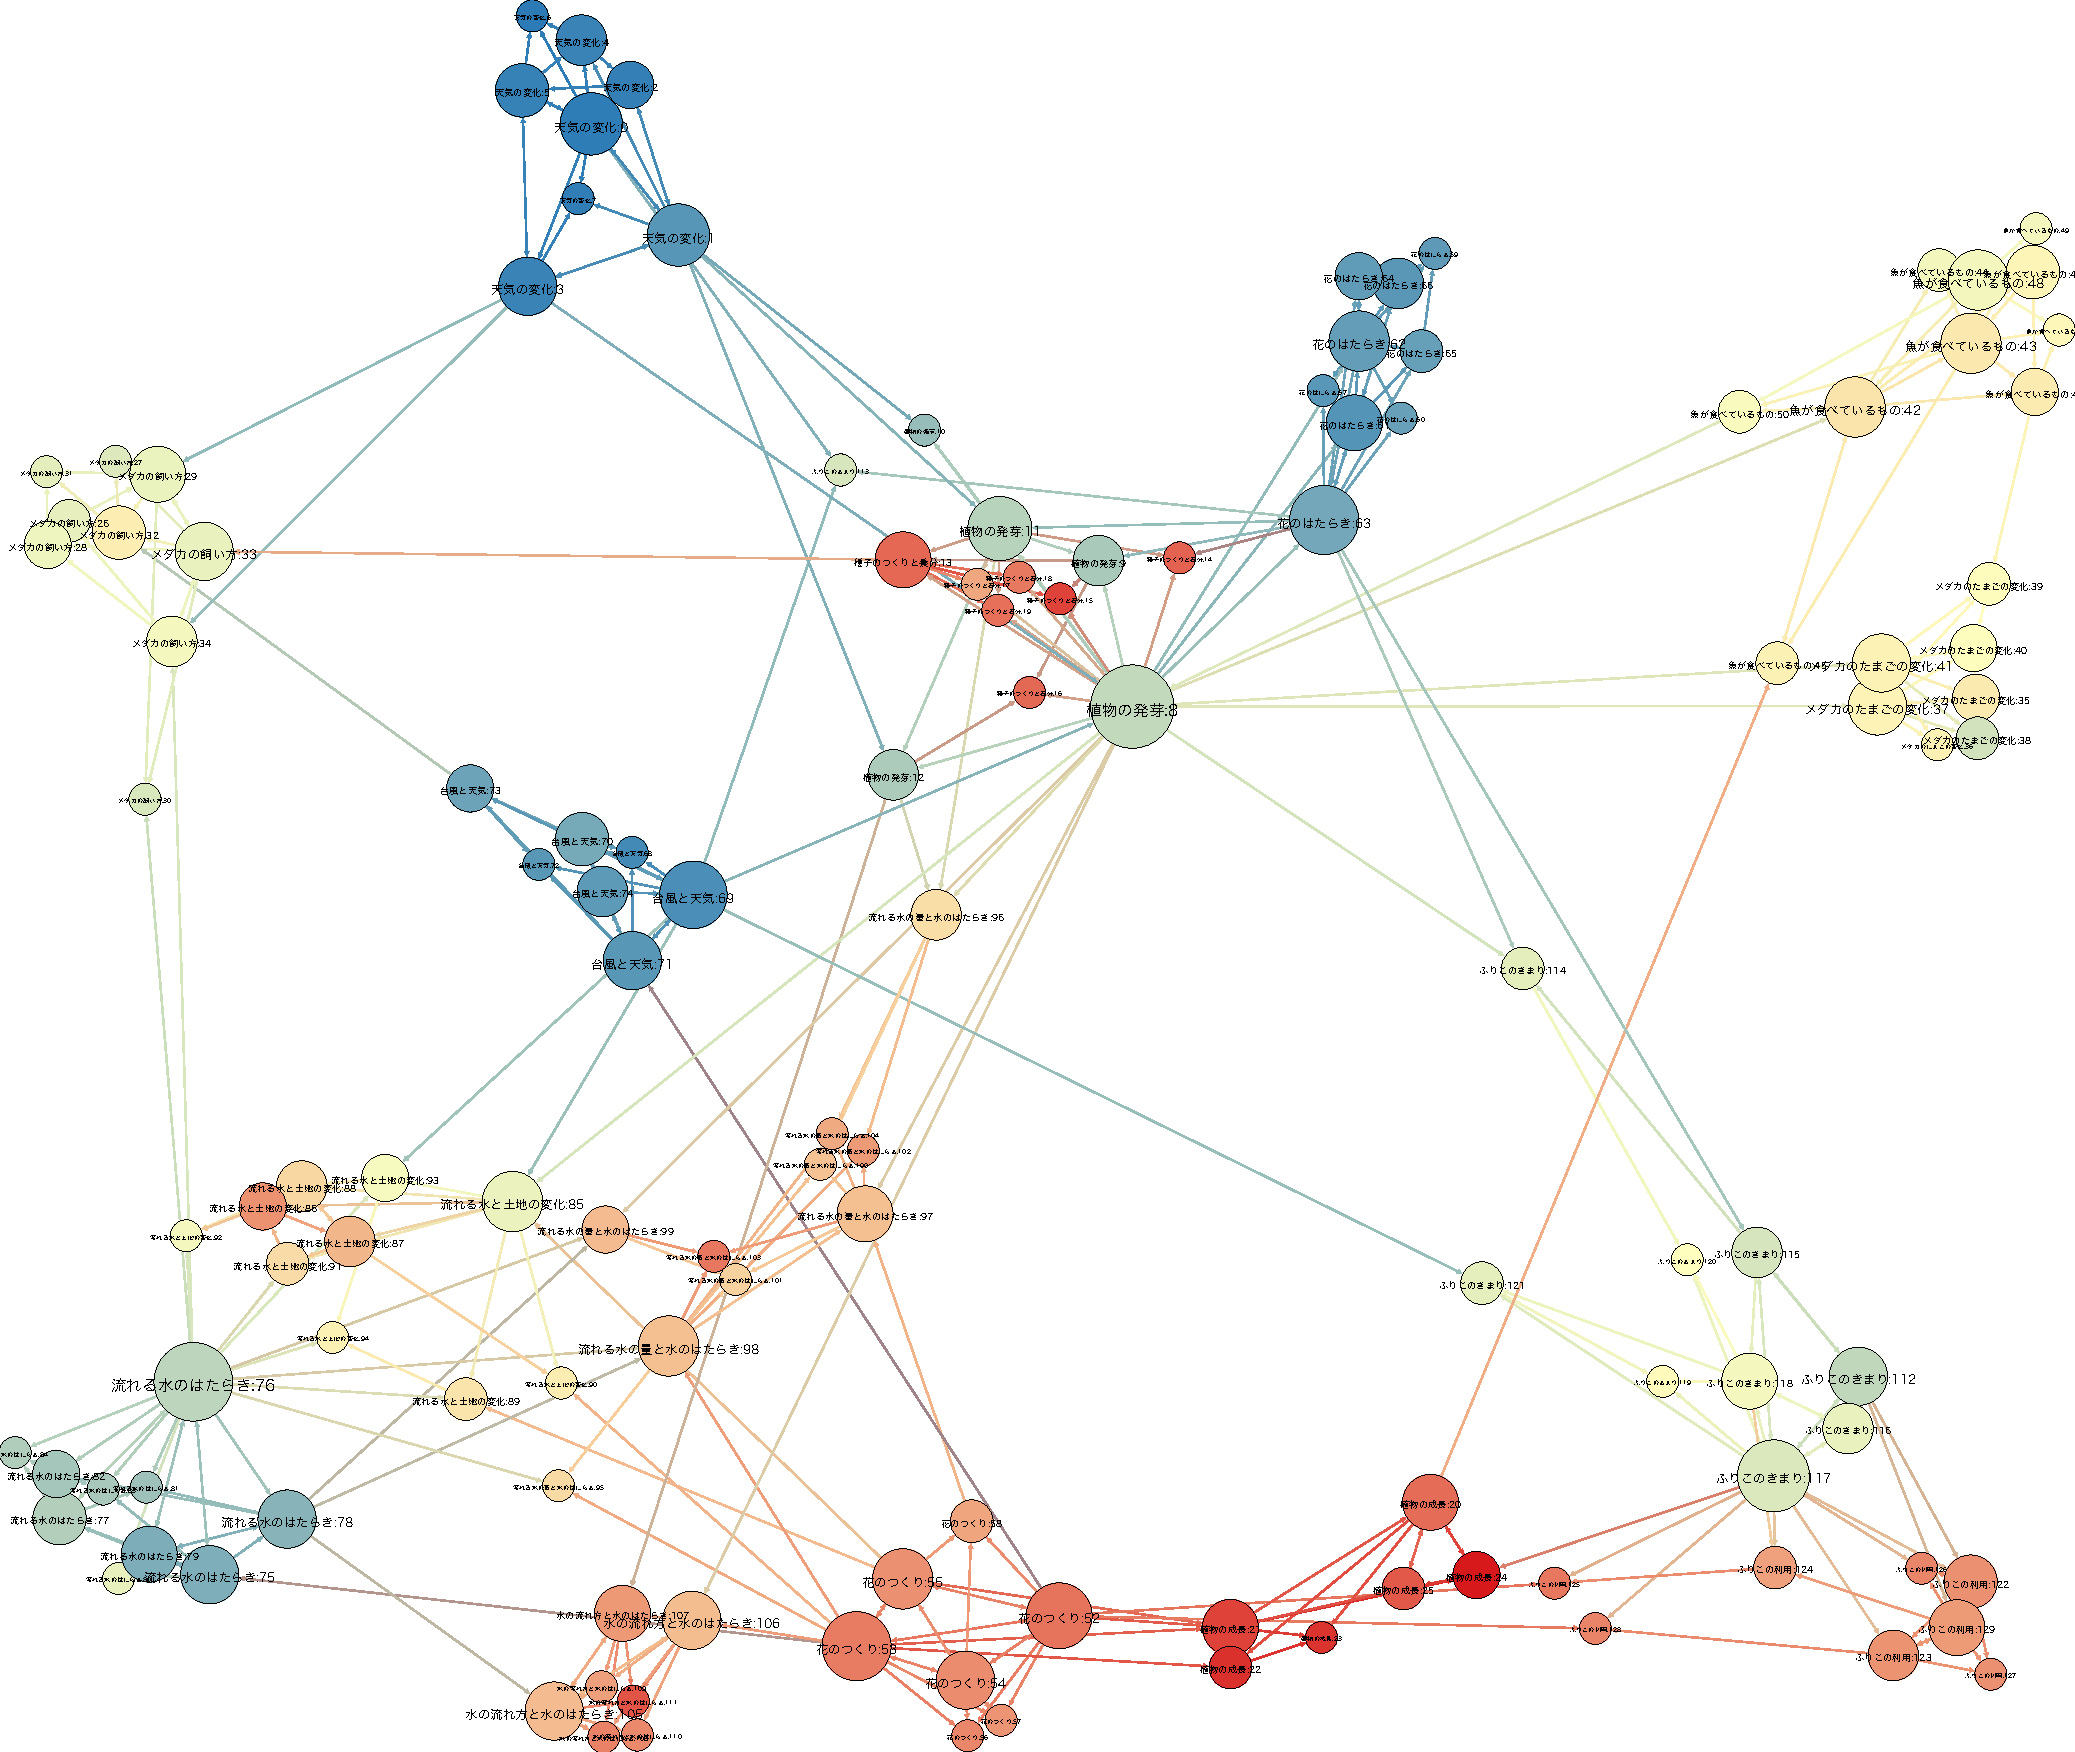
\includegraphics[width=200pt, height=200pt]{./img/net_s5sci.pdf}
			\caption{小学5年理科の問題間関係ネットワーク}
			\label{fig:net_s5sci}
		\endminipage\hfill
	}
\end{center}
\end{figure}

\begin{figure}[!htb]
\begin{center}
	\hspace*{-10pt}\makebox[1.2\textwidth][c]{
		\minipage{0.52\textwidth}
			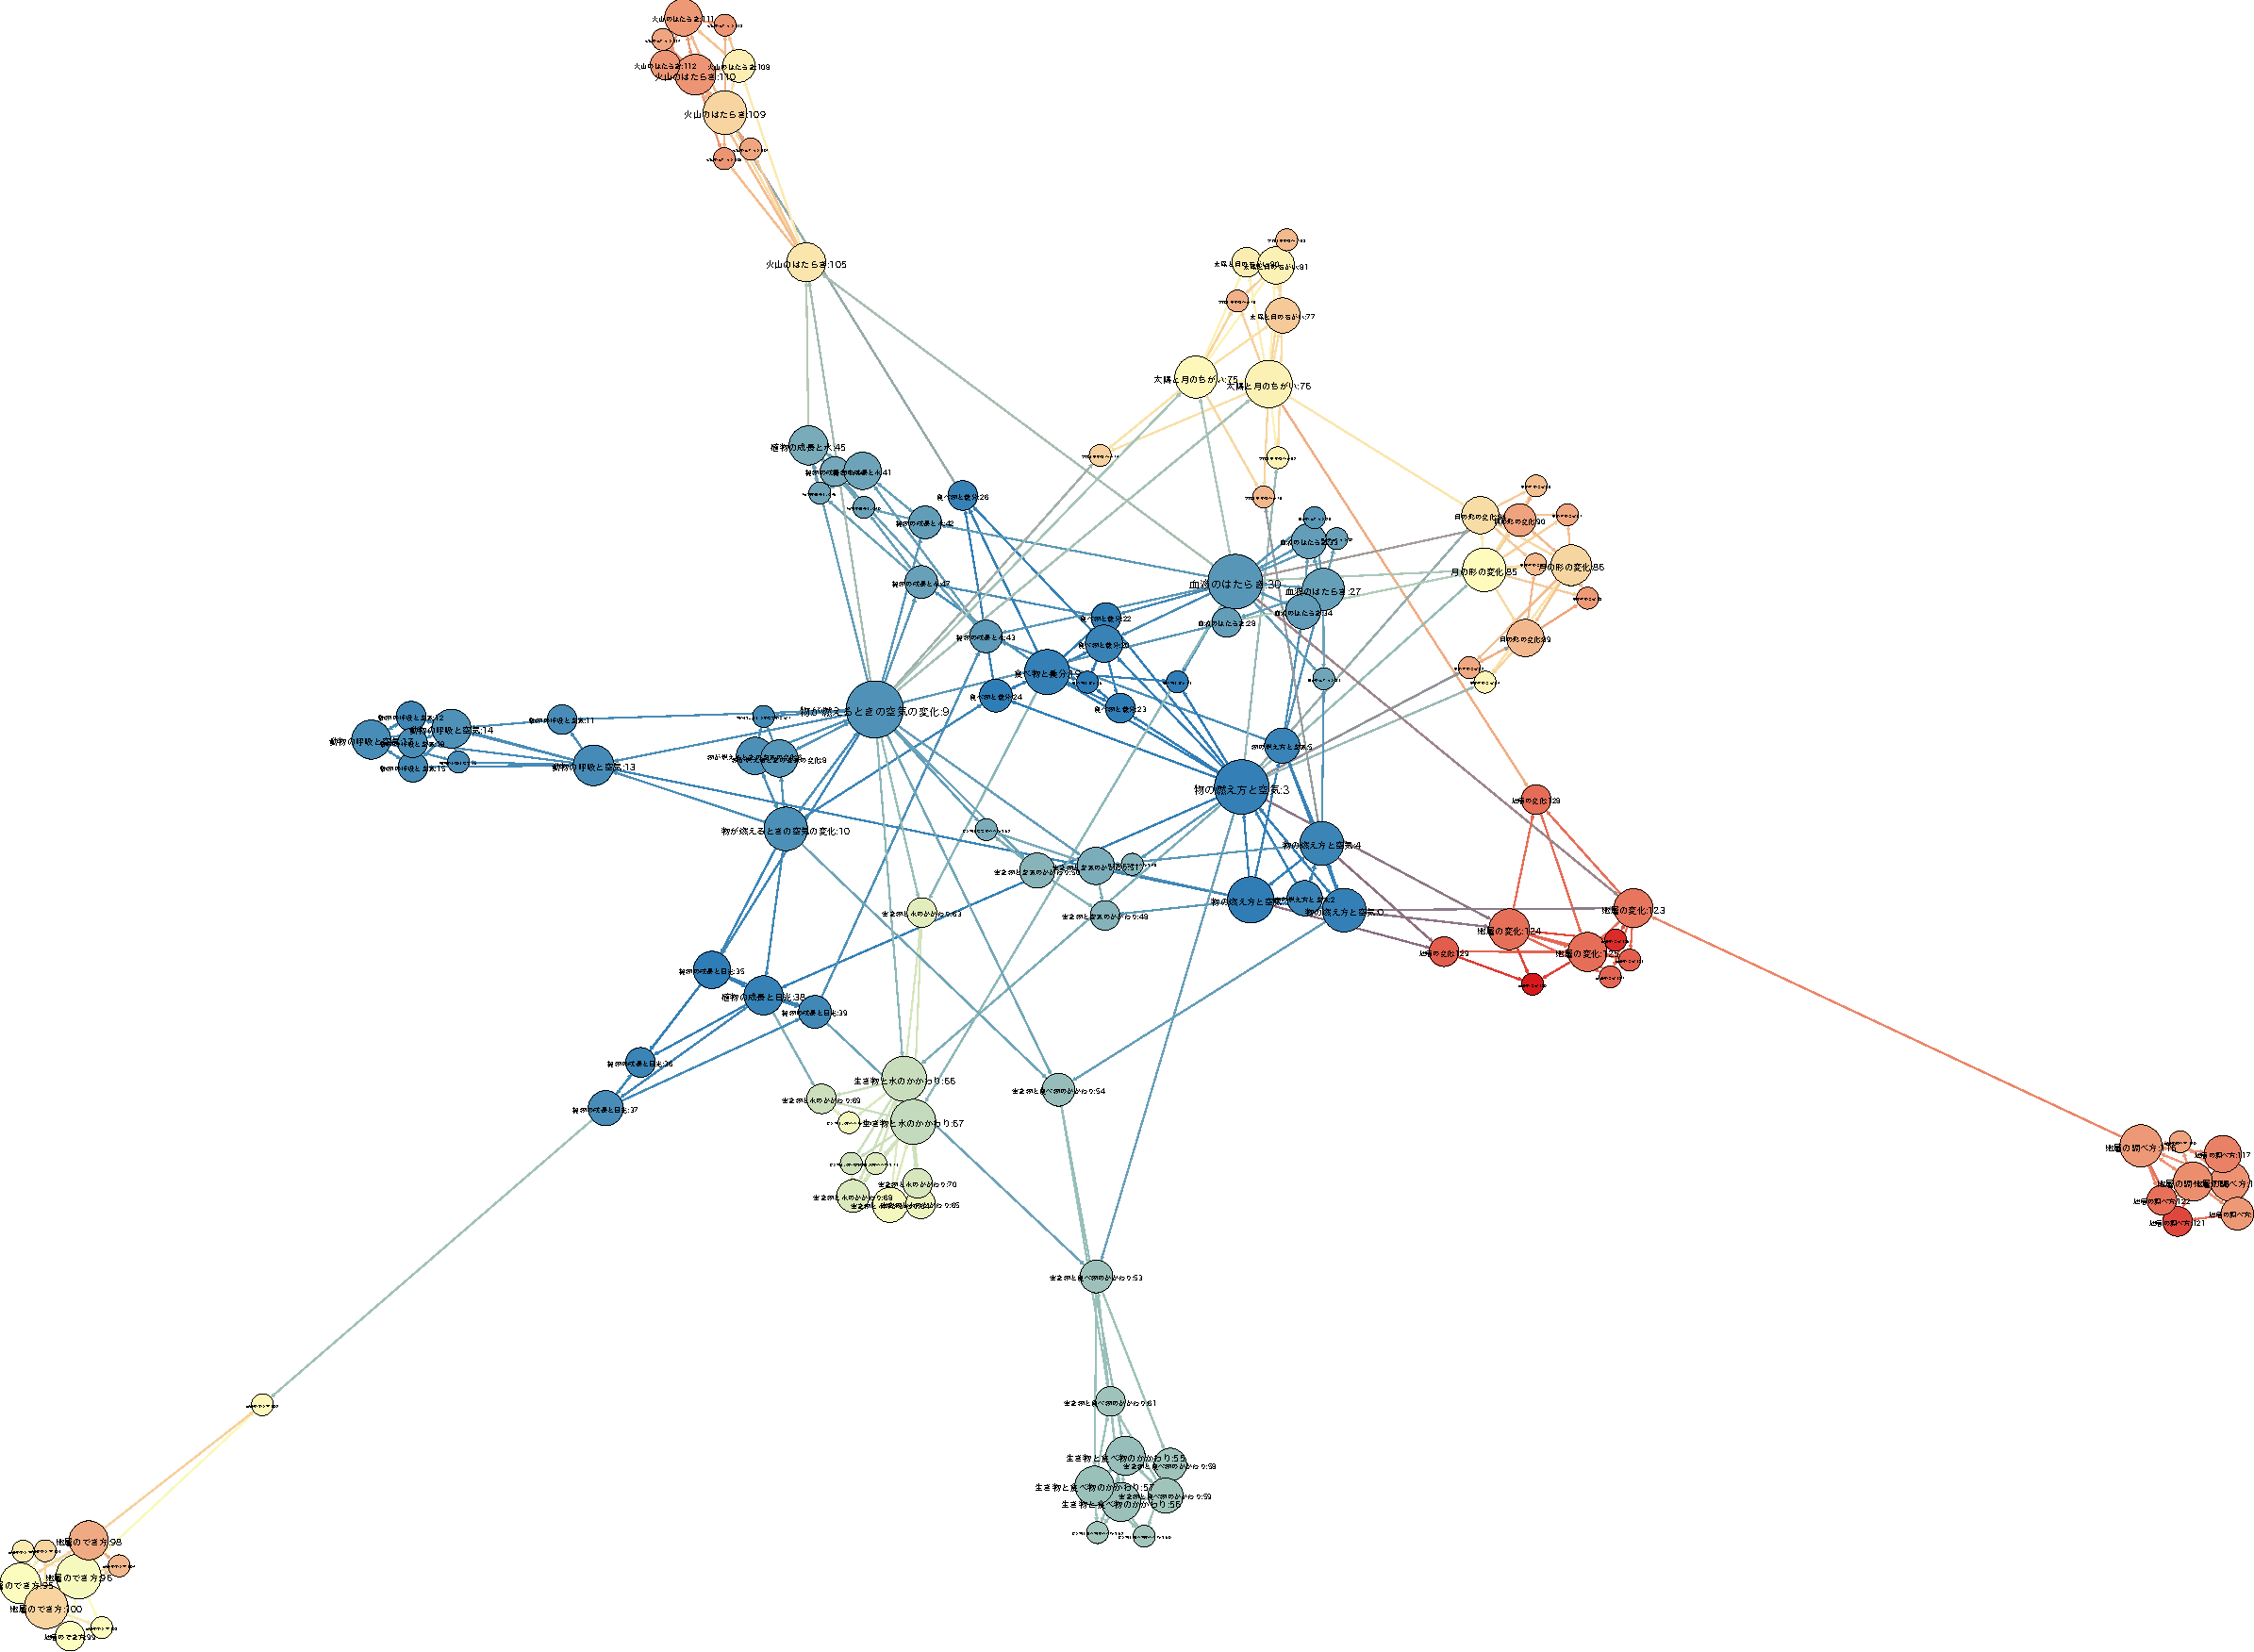
\includegraphics[width=200pt, height=200pt]{./img/net_s6sci.pdf}
			\caption{小学6年理科の問題間関係ネットワーク}
			\label{fig:net_s6_sci}
		\endminipage\hfill
		\minipage{0.52\textwidth}
			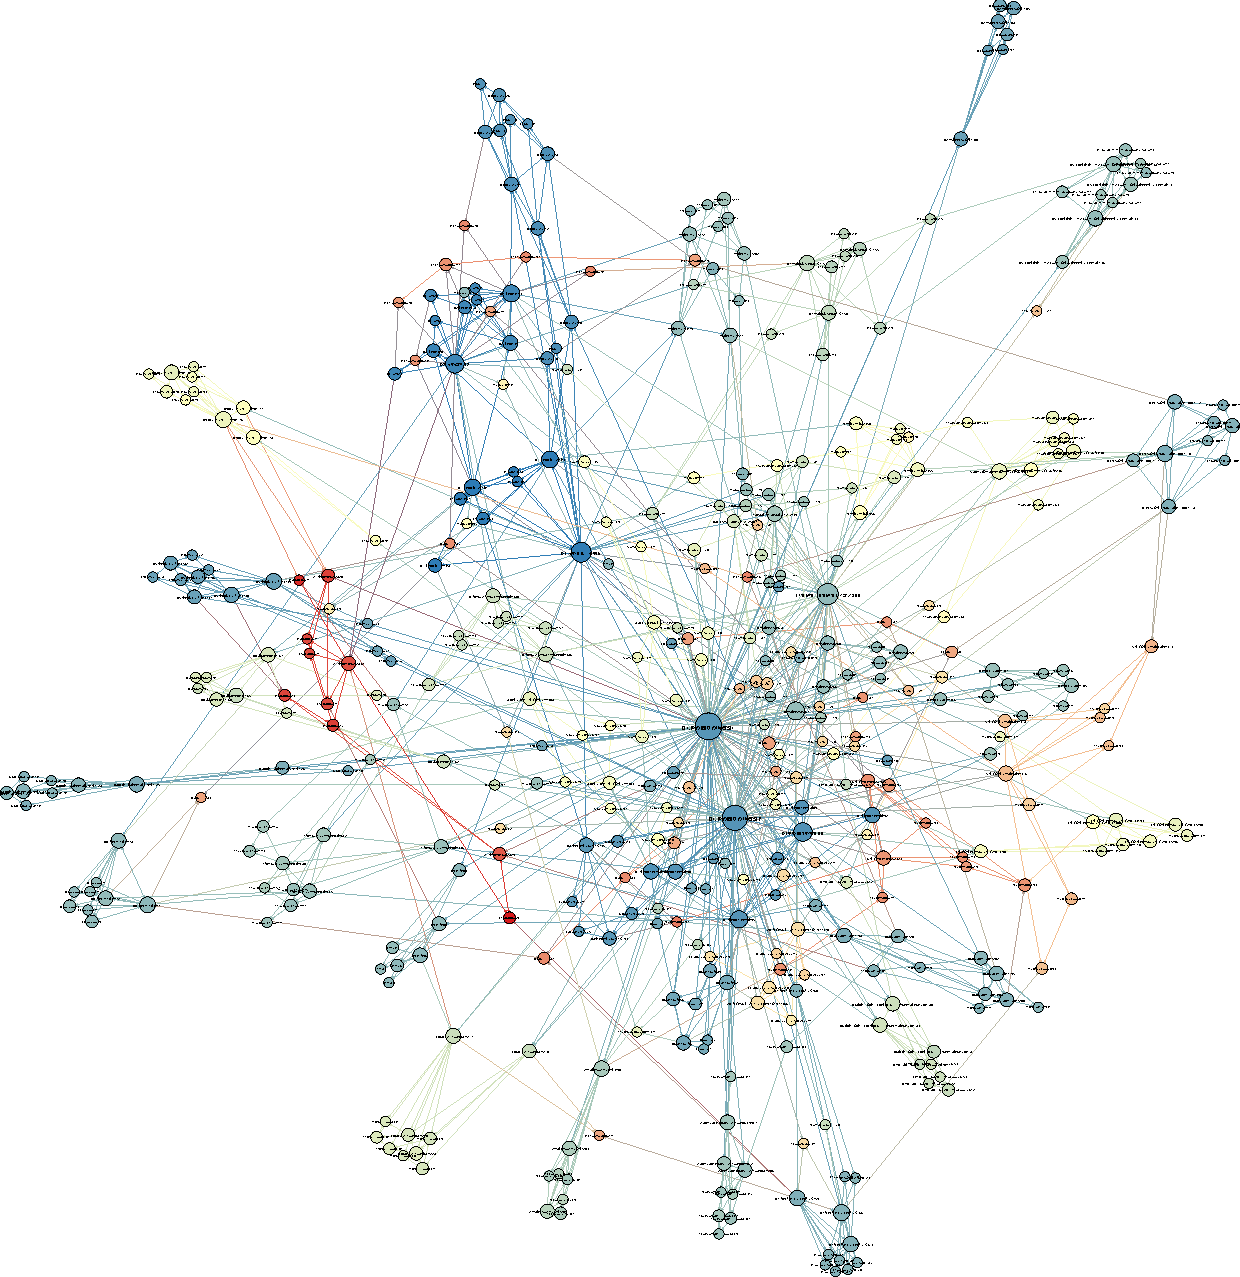
\includegraphics[width=200pt, height=200pt]{./img/net_c_sci1.pdf}
			\caption{中学理科1の問題間関係ネットワーク}
			\label{fig:net_c_sci1}
		\endminipage\hfill
	}
	\hspace*{-10pt}\makebox[1.2\textwidth][c]{
		\minipage{0.52\textwidth}
			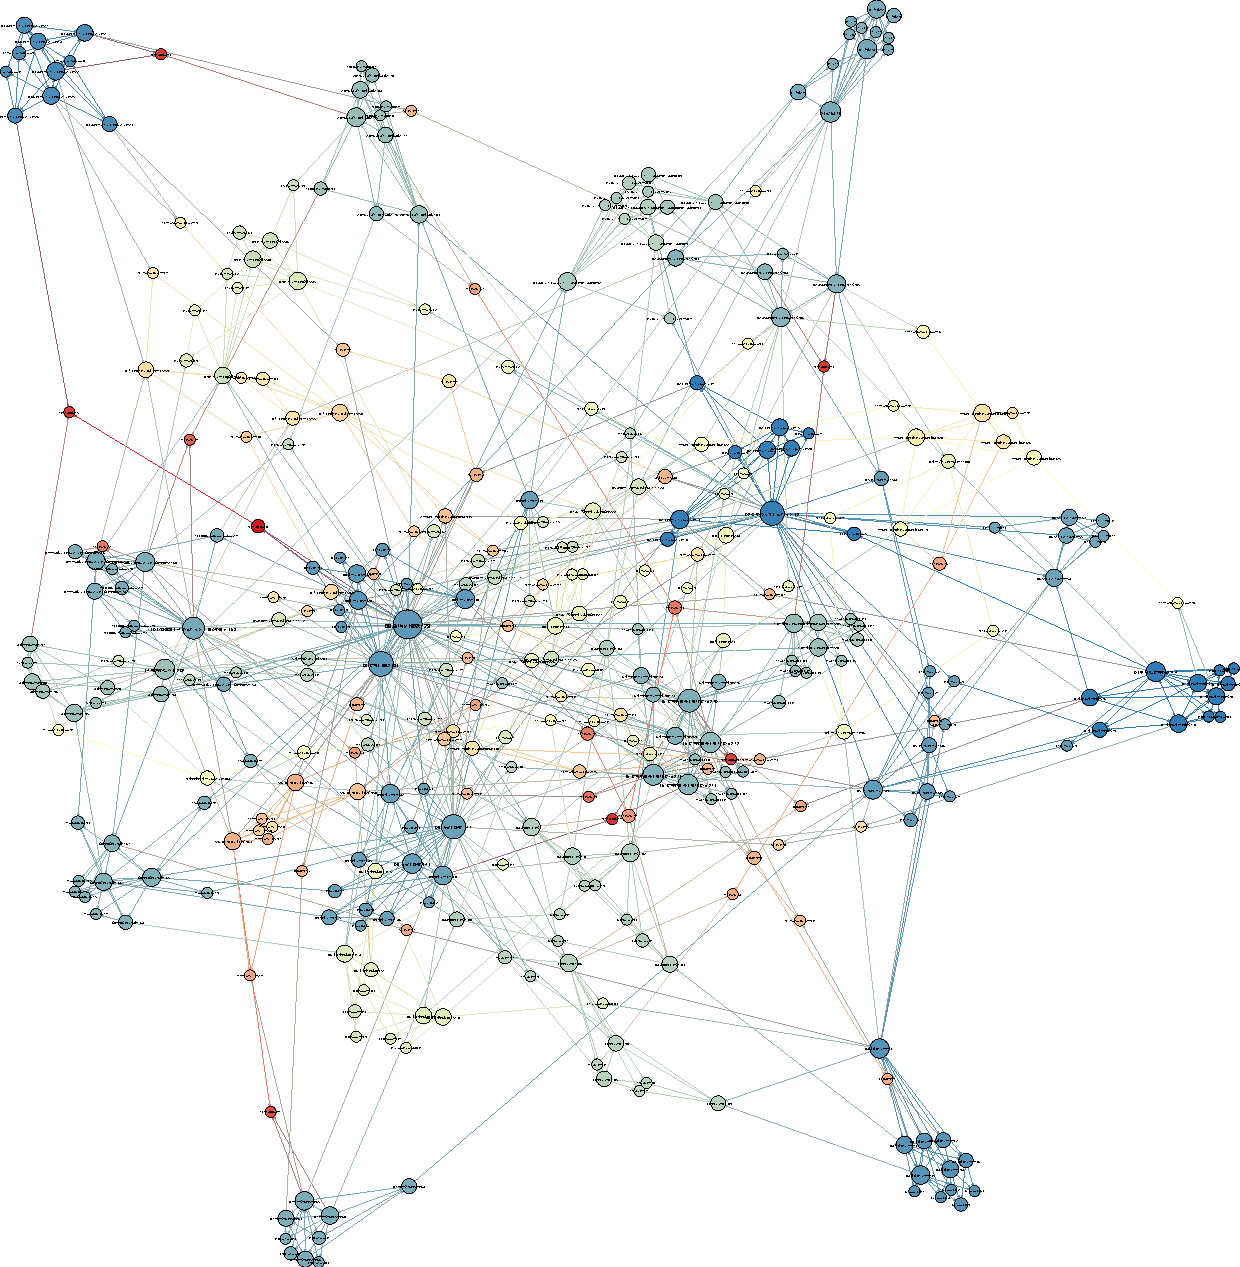
\includegraphics[width=200pt, height=200pt]{./img/net_c_sci2.pdf}
			\caption{中学理科2の問題間関係ネットワーク}
			\label{fig:net_c_sci2}
		\endminipage\hfill
		%\endminipage\hfill
	}
\end{center}
\end{figure}


\begin{figure}[!htb]
\begin{center}
	\hspace*{-10pt}\makebox[1.2\textwidth][c]{
		\minipage{0.52\textwidth}
			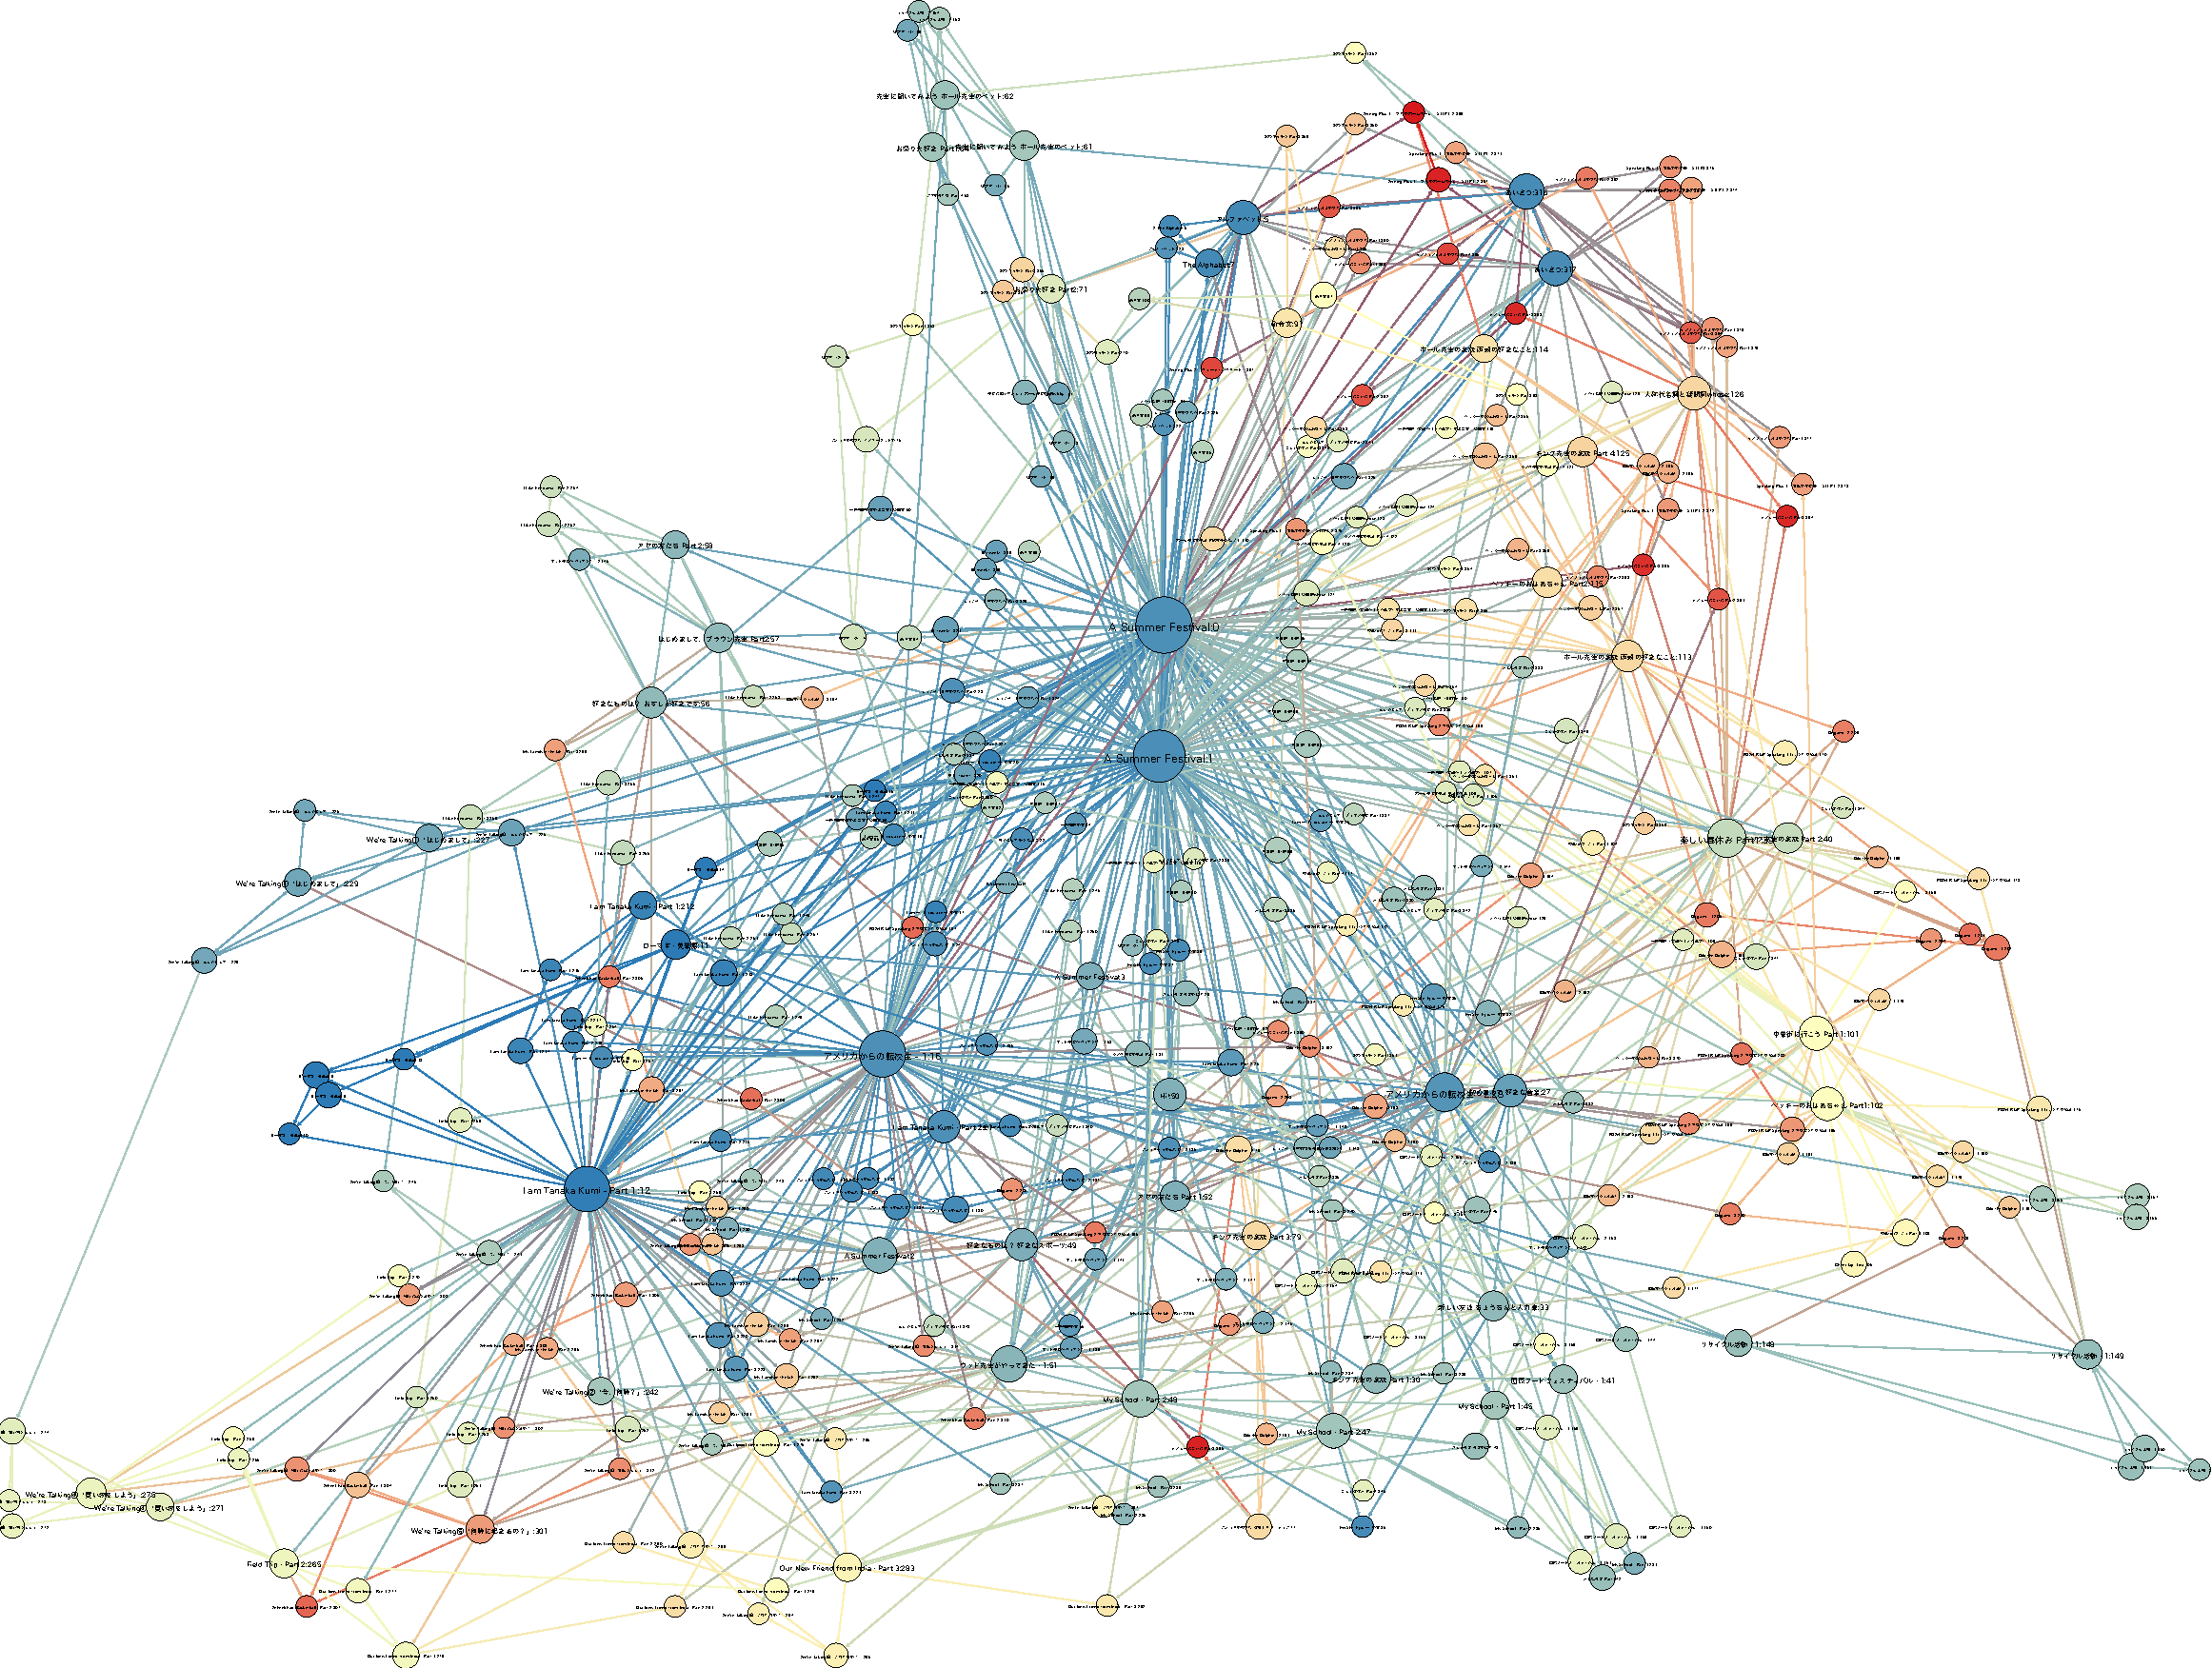
\includegraphics[width=200pt, height=200pt]{./img/net_c1eng.pdf}
			\caption{中学1年英語の問題間関係ネットワーク}
			\label{fig:net_c1eng}
		\endminipage\hfill
		\minipage{0.52\textwidth}
			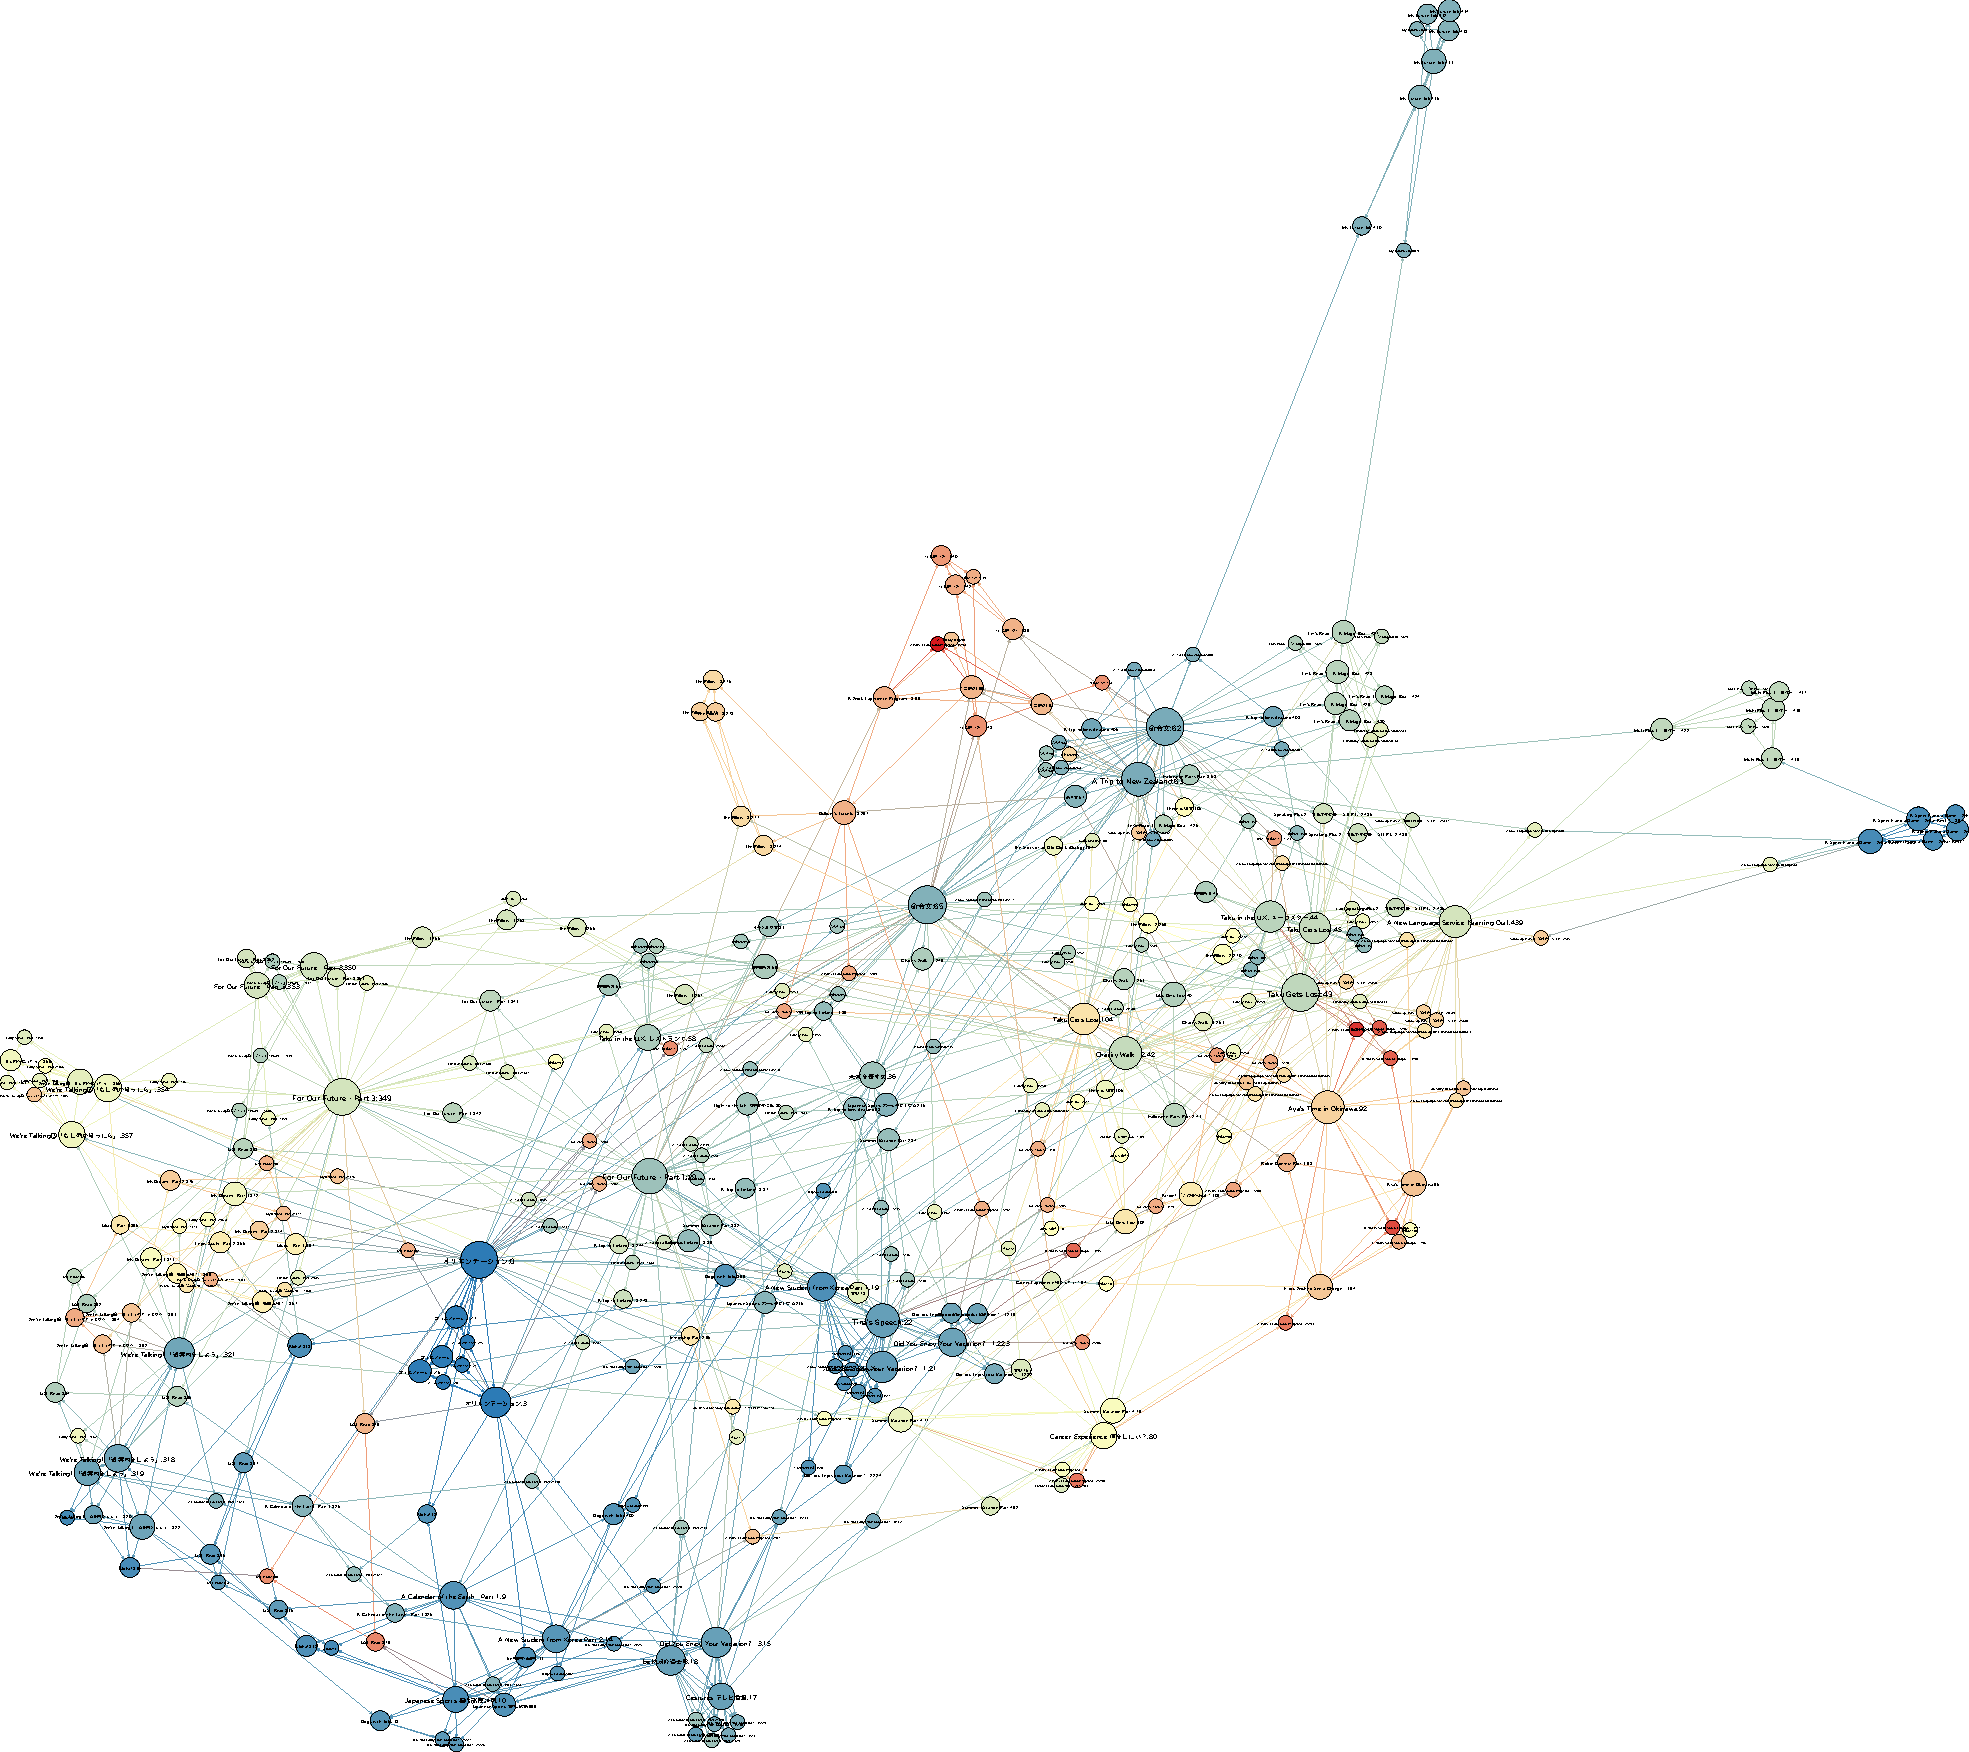
\includegraphics[width=200pt, height=200pt]{./img/net_c2eng.pdf}
			\caption{中学2年英語の問題間関係ネットワーク}
			\label{fig:net_c2eng}
		\endminipage\hfill
	}
	\hspace*{-10pt}\makebox[1.2\textwidth][c]{
		\minipage{0.52\textwidth}
			\includegraphics[width=200pt, height=200pt]{./img/net_c3eng.pdf}
			\caption{中学3年英語の問題間関係ネットワーク}
			\label{fig:net_c3eng}
		\endminipage\hfill
		%\endminipage\hfill
	}
\end{center}
\end{figure}


\addcontentsline{toc}{chapter}{謝辞}
\chapter*{謝辞}
\fancyhf{}
\rhead{}
\lhead{}
\cfoot{\thepage}

本研究の遂行や本論文の執筆にあたり,非常に多くの方からご指導,ご支援をいただきました.
心より御礼申し上げます.

指導教官である松尾豊特任准教授には,
研究構想の相談や論文の書き方,本論文の論理構成について,貴重なご指導をいただきました.
ここに,深く謝意を表します.

分析サーバやGPU解析環境の用意等,物理的な研究環境の構築に多大なご協力を下さった
研究室の教官である中山浩太郎先生に,
深く感謝致します.

上野山勝也助教授には,
研究の方向性や論文の構成について,
多大なご指導をいただきました.
深く感謝致します.

松尾研究室やGCIの皆様には,多大なご協力,ご支援いただきました.
秘書の中野佐恵子さん,永本登代子さん,浪岡亮子さん,木全弥栄さんは,日頃から研究室の環境を整えて下さり,研究生活を支えてくださいました.
松尾研究室の博士・修士課程の先輩である岩澤有祐さん,飯塚修平さん,野中尚輝さん,鈴木雅大さん,金子貴輝さん,那須野薫さん,黒滝紘生さん,保住純さん,冨山翔司さんには,
研究の相談に幾度も乗っていただき,多大なご助力をいただきました.
特に,研究テーマや,研究全体の設計について何度も相談に応じていただいたことに加え,
日常の議論を通じて多くの知識や示唆をいただいた那須野薫さんには,多大なるご助力に深く感謝致します.
研究室の同期である大野峻典氏,田村浩一郎氏は,卒業論文の構想や執筆に関して率直に意見を交わし,互いに切磋琢磨し合いながら研究を進めさせていただきました.

ここに,松尾研究室の皆様へ謝意を表します.
\vvspace

\begin{flushright}
東京大学工学部\\
システム創成学科知能社会システムコース\\
松尾研究室 学部4年\\
中川大海\\
平成29年3月\\
\end{flushright}


\end{document}

